% !TeX root = ../thesis.tex
\chapter{Grundlagen}
\label{chap:fundamentals_related-work}
In diesem Kapitel werden die Grundlagen eines neuartigen Übertragungssystems vorgestellt. Da eine Audioübertragung mittels \gls{acr:VLC}-Technik implementiert werden soll, wird zunächst auf die Eigenschaften eines zu übertragenden Audiosignals eingegangen. Darauf folgend werden einige Grundlagen zur Übertragungstechnik und der verwendeten elektronischen Bauteile erläutert. Zuletzt setzt sich dieses Kapitel mit Programmen auseinander, welche signifikant für die Realisierung der Übertragung sind. Hier werden grundlegende Funktionsweisen, sowie deren Rolle in der analogen und digitalen Signalverarbeitung thematisiert. 

\section{Eigenschaften von Audiosignalen}
\label{subsec:audio}

Ziel der vorliegenden Abschlussarbeit ist die Übertragung eines Echtzeit-Audio-Signals mithilfe des projektierten \gls{acr:VLC}-Senders. Deshalb soll im nachfolgenden Kapitel anfänglich im Allgemeinen auf die Übertragung von Audiosignalen eingegangen werden. Praktische Beispiele zu der Übertragung von Audiosignalen über größere Entfernung ergeben sich bei der Übertragung von Sprache und Musik. Hierbei wird zunächst der Hörschall mit Hilfe eines Mikrofons in ein proportionales elektrisches Signal umgewandelt. Dieses Signal wird anschließend auf drahtlosem  Wege dem Empfänger übermittelt. Gängige Beispiele für die drahtlose Übertragung sind \gls{acr:WLAN} und das klassische DAB+. Am Empfangsort wird das elektrische Signal mittels eines Lautsprechers wieder in ein akustisches Signal umgesetzt.\cite{plassmannHandbuchElektrotechnik2016} Der Lautsprecher erzeugt eine mechanische Welle, die in Hörschall resultiert. Hierbei definiert die Frequenz eine Tonlage und die Amplitude, in diesem Fall, die Lautstärke des Audiosignals. Beim Auftreffen dieser mechanischen Welle auf das menschliche Trommelfell wird dieses in Schwingung versetzt und regt somit die menschlichen Nerven an. Das Signal wird im Ohr von einer mechanischen Welle in ein elektrisches Signal umgewandelt, das über die Nervenbahnen zum Gehirn gelangt. Im Gehirn wird das elektrische Signal verarbeitet und mit semantischen Informationen verbunden. Diese ermöglichen das menschliche Hören.\cite{stotzaudio} Die Wahrnehmung von Tönen bei Menschen hängt jedoch nicht nur von der Amplitude und der Frequenz des Tones ab, sondern auch von der wahrnehmenden Person selbst. Demnach können Menschen nur Töne in einem bestimmten Frequenzbereich wahrnehmen. Frequenzen unterhalb des menschlichen Hörbereichs werden Infraschall genannt, darüber liegende Frequenzen werden als Ultraschall bezeichnet. Dieser Frequenzbereich ist nicht nur von Mensch zu Mensch unterschiedlich, sondern variiert auch mit zunehmendem Alter. Daher kann der Frequenzbereich des menschlichen Hörens nicht pauschal vereinheitlicht werden. Plassmann bringt den Hörbereich zwischen 16 Hz und 16 kHz vor \cite{plassmannHandbuchElektrotechnik2016}, wohingegen Michels ihn zwischen 16 Hz bis 20 kHz ansiedelt \cite{michelsSonographieOrganUnd2012}. Der hörbare Frequenzbereich variiert auch von Lebewesen zu Lebewesen. Hunde haben zum Beispiel ein erheblich feineres Hörorgan als Menschen. Ihr Frequenzbereich erstreckt sich als Folge dessen von 65 Hz bis 45 kHz.\cite{michelsSonographieOrganUnd2012}

\begin{figure}[H]
	\centering
	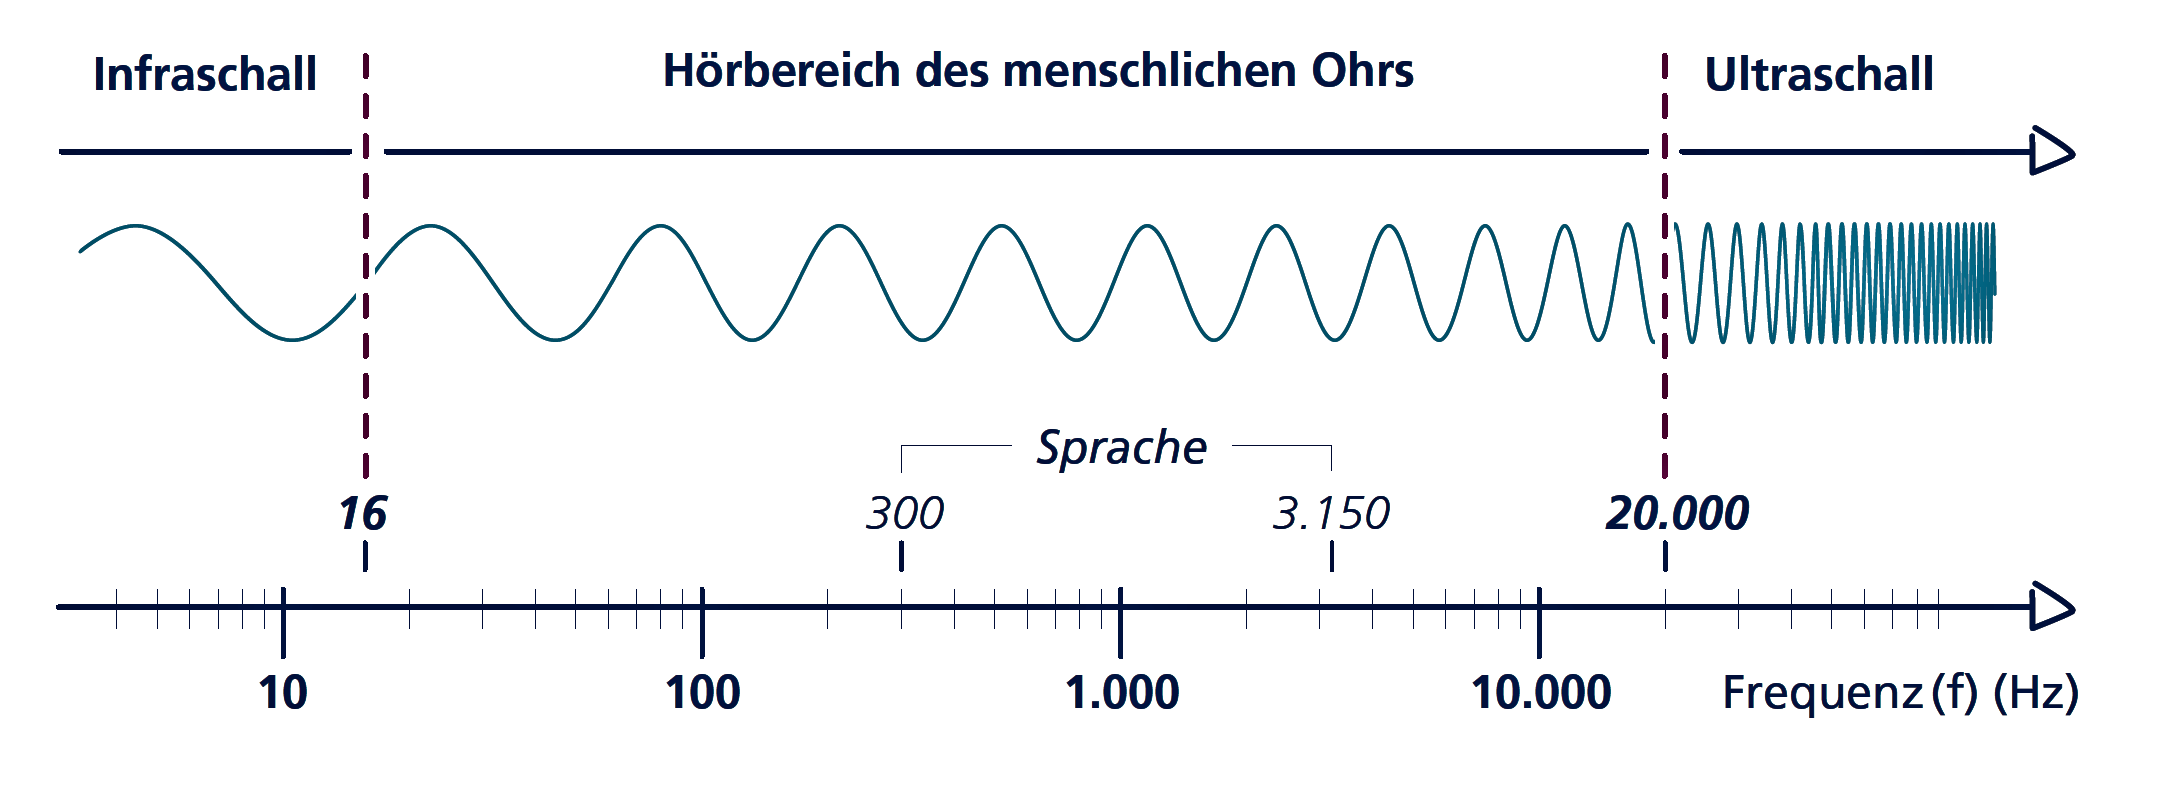
\includegraphics[width=1\textwidth]{audiospektrum.png}
	\caption[Hörbereich des menschlichen Ohres]{Hörbereich des menschlichen Ohres} \cite{michelsSonographieOrganUnd2012}
	\label{fig:audiospektrum}
\end{figure}

Außerdem verändert der Abstand zu einer Quelle zusätzlich die Wahrnehmung des Signals. Die Amplitude einer sich ausbreitenden Welle verringert sich mit zunehmender Distanz, wodurch die Lautstärke abnimmt. Befindet sich eine Quelle außerhalb der Hörreichweite können dessen gesendete Wellen durch analoge oder digitale Kommunikationssysteme abgefangen werden, um eine Übertragung zu ermöglichen. Zur Übertragung und Weiterverarbeitung der beschriebenen mechanischen Welle muss diese zunächst in eine elektrische Größe verwandelt werden. Bei dieser Wandlung wird für Audiosignale ein Mikrofon verwendet. Ähnlich wie es mit dem Trommelfell im menschlichen Ohr passiert, wird im Inneren des Mikrofons eine Membran in Schwingung versetzt und erzeugt dadurch eine elektrische analoge Spannung.
Zur digitalen Verarbeitung des Signals muss dieses mithilfe eines \gls{acr:AD}-Wandlers in digitale Werte verwandelt werden. Hierfür wird die Analogspannung in zeitlich äquidistanten Abständen ausgewertet und abgespeichert. Es wird also ein Signal mit einem Dirac-Kamm multipliziert um dessen Werte zu ermitteln. Dieser Vorgang wird Abtastung genannt und in Darstellung~\ref{fig:abtastung} näher veranschaulicht. Durch die Ausblendeigenschaft der Impulsfunktion bleiben nach der Multiplikation nur noch die Werte des Signals zu den Abtastzeitpunkten übrig. Zwischen den Abtastzeitpunkten wird jedoch keine Information abgefragt, wodurch der Wert an diesen Stellen Null beträgt. Zur Rekonstruierung des Originalsignals müssen durch einen Digital-Analog-Wandler die fehlenden Signalabschnitte interpoliert werden. Um also eine aussagekräftige Abtastung durchzuführen, ist die Korrelation zwischen Abtastfrequenz und Signalfrequenz zu berücksichtigen.


\begin{figure}[H]
	\centering
	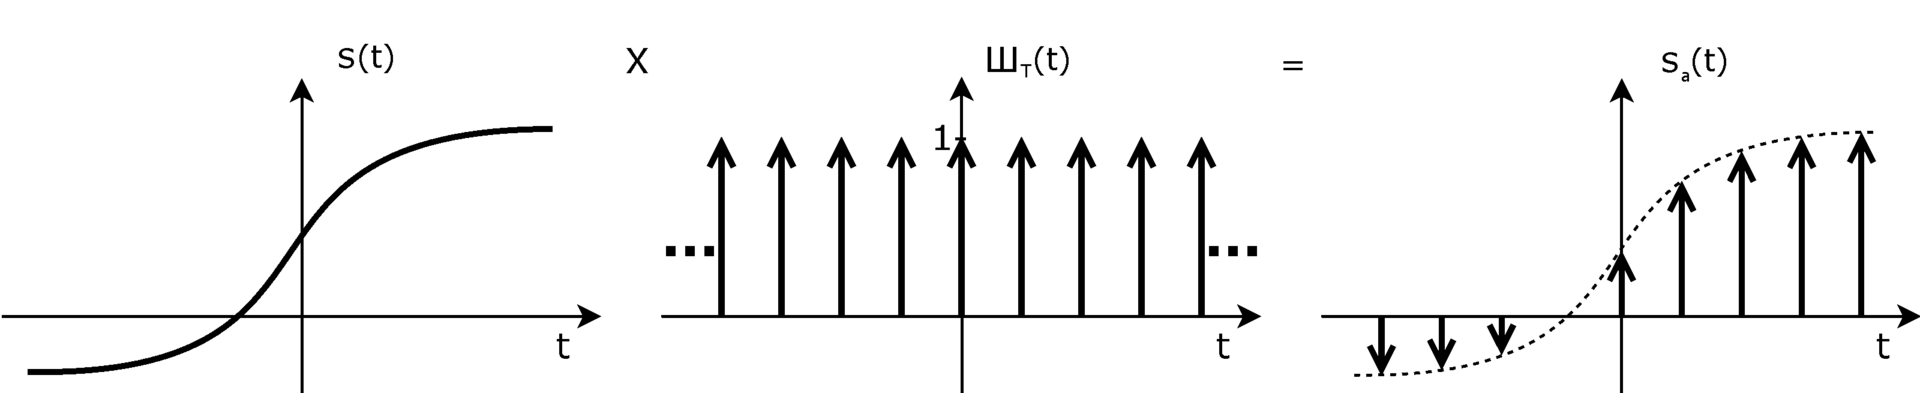
\includegraphics[width=1\textwidth]{abtastung.png}
	\caption[Abtastung eines Signals]{Abtastung eines Signals} \gls{online:abtastung}
	\label{fig:abtastung}
\end{figure}

In Abbildung~\ref{fig:abtastung} ist zu erkennen, dass genügend Abtastwerte vorhanden sind, weshalb der Verlauf des Signals im Nachgang detailliert wiedergegeben werden kann. Abtastfrequenz und Signalfrequenz stehen demnach in einem adäquaten Verhältnis zueinander. Je weniger Abtastwerte vorhanden sind, desto größer werden Messabstände. Dies hat zur Folge, dass eine Rekonstruktion des Signales bald nicht mehr möglich ist.\cite{masteraudio}

Das Abtasttheorem von Shannon besagt, dass für die höchste Signalfrequenz pro Schwingung mindestens zwei mal abgetastet werden muss, um das Signal ausreichend rekonstruieren zu können. Hierbei wird also Formel~\ref{equ:abtast} angewendet.

\begin{equation}
	\label{equ:abtast}
	F_{A} \geq 2 \cdot F_{S}
\end{equation}

Die Variable $F_{A}$ bildet hierbei die Abtastfrequenz ab und $F_{S}$ steht für die höchste im Signal enthaltende Frequenz. In Abbildung~\ref{fig:shannon} wird bei der oberen Abtastung die Regel von Shannon befolgt, wohingegen sie im unteren Teil der Abbildung verletzt wird. An diesem Beispiel ist gut zu erkennen, dass durch die richtige Abtastung eine relativ originalgetreue Rekonstruktion stattfinden kann, während bei einer Unterabtastung das Signal merklich verfälscht rekonstruiert wird. Zuzüglich ist an dieser Darstellung jedoch zu sehen, dass die Abtastung nur den minimalen und den maximalen Wert des Signals abgetastet hat.\cite{shannon} Dies bedeutet, dass bei einer Phasenverschiebung von $90^\circ$ nur Nulldurchgänge des Signals abgetastet geworden sind, was eine Rekonstruktion unmöglich gemacht hätte. 

\begin{figure}[H]
	\centering
	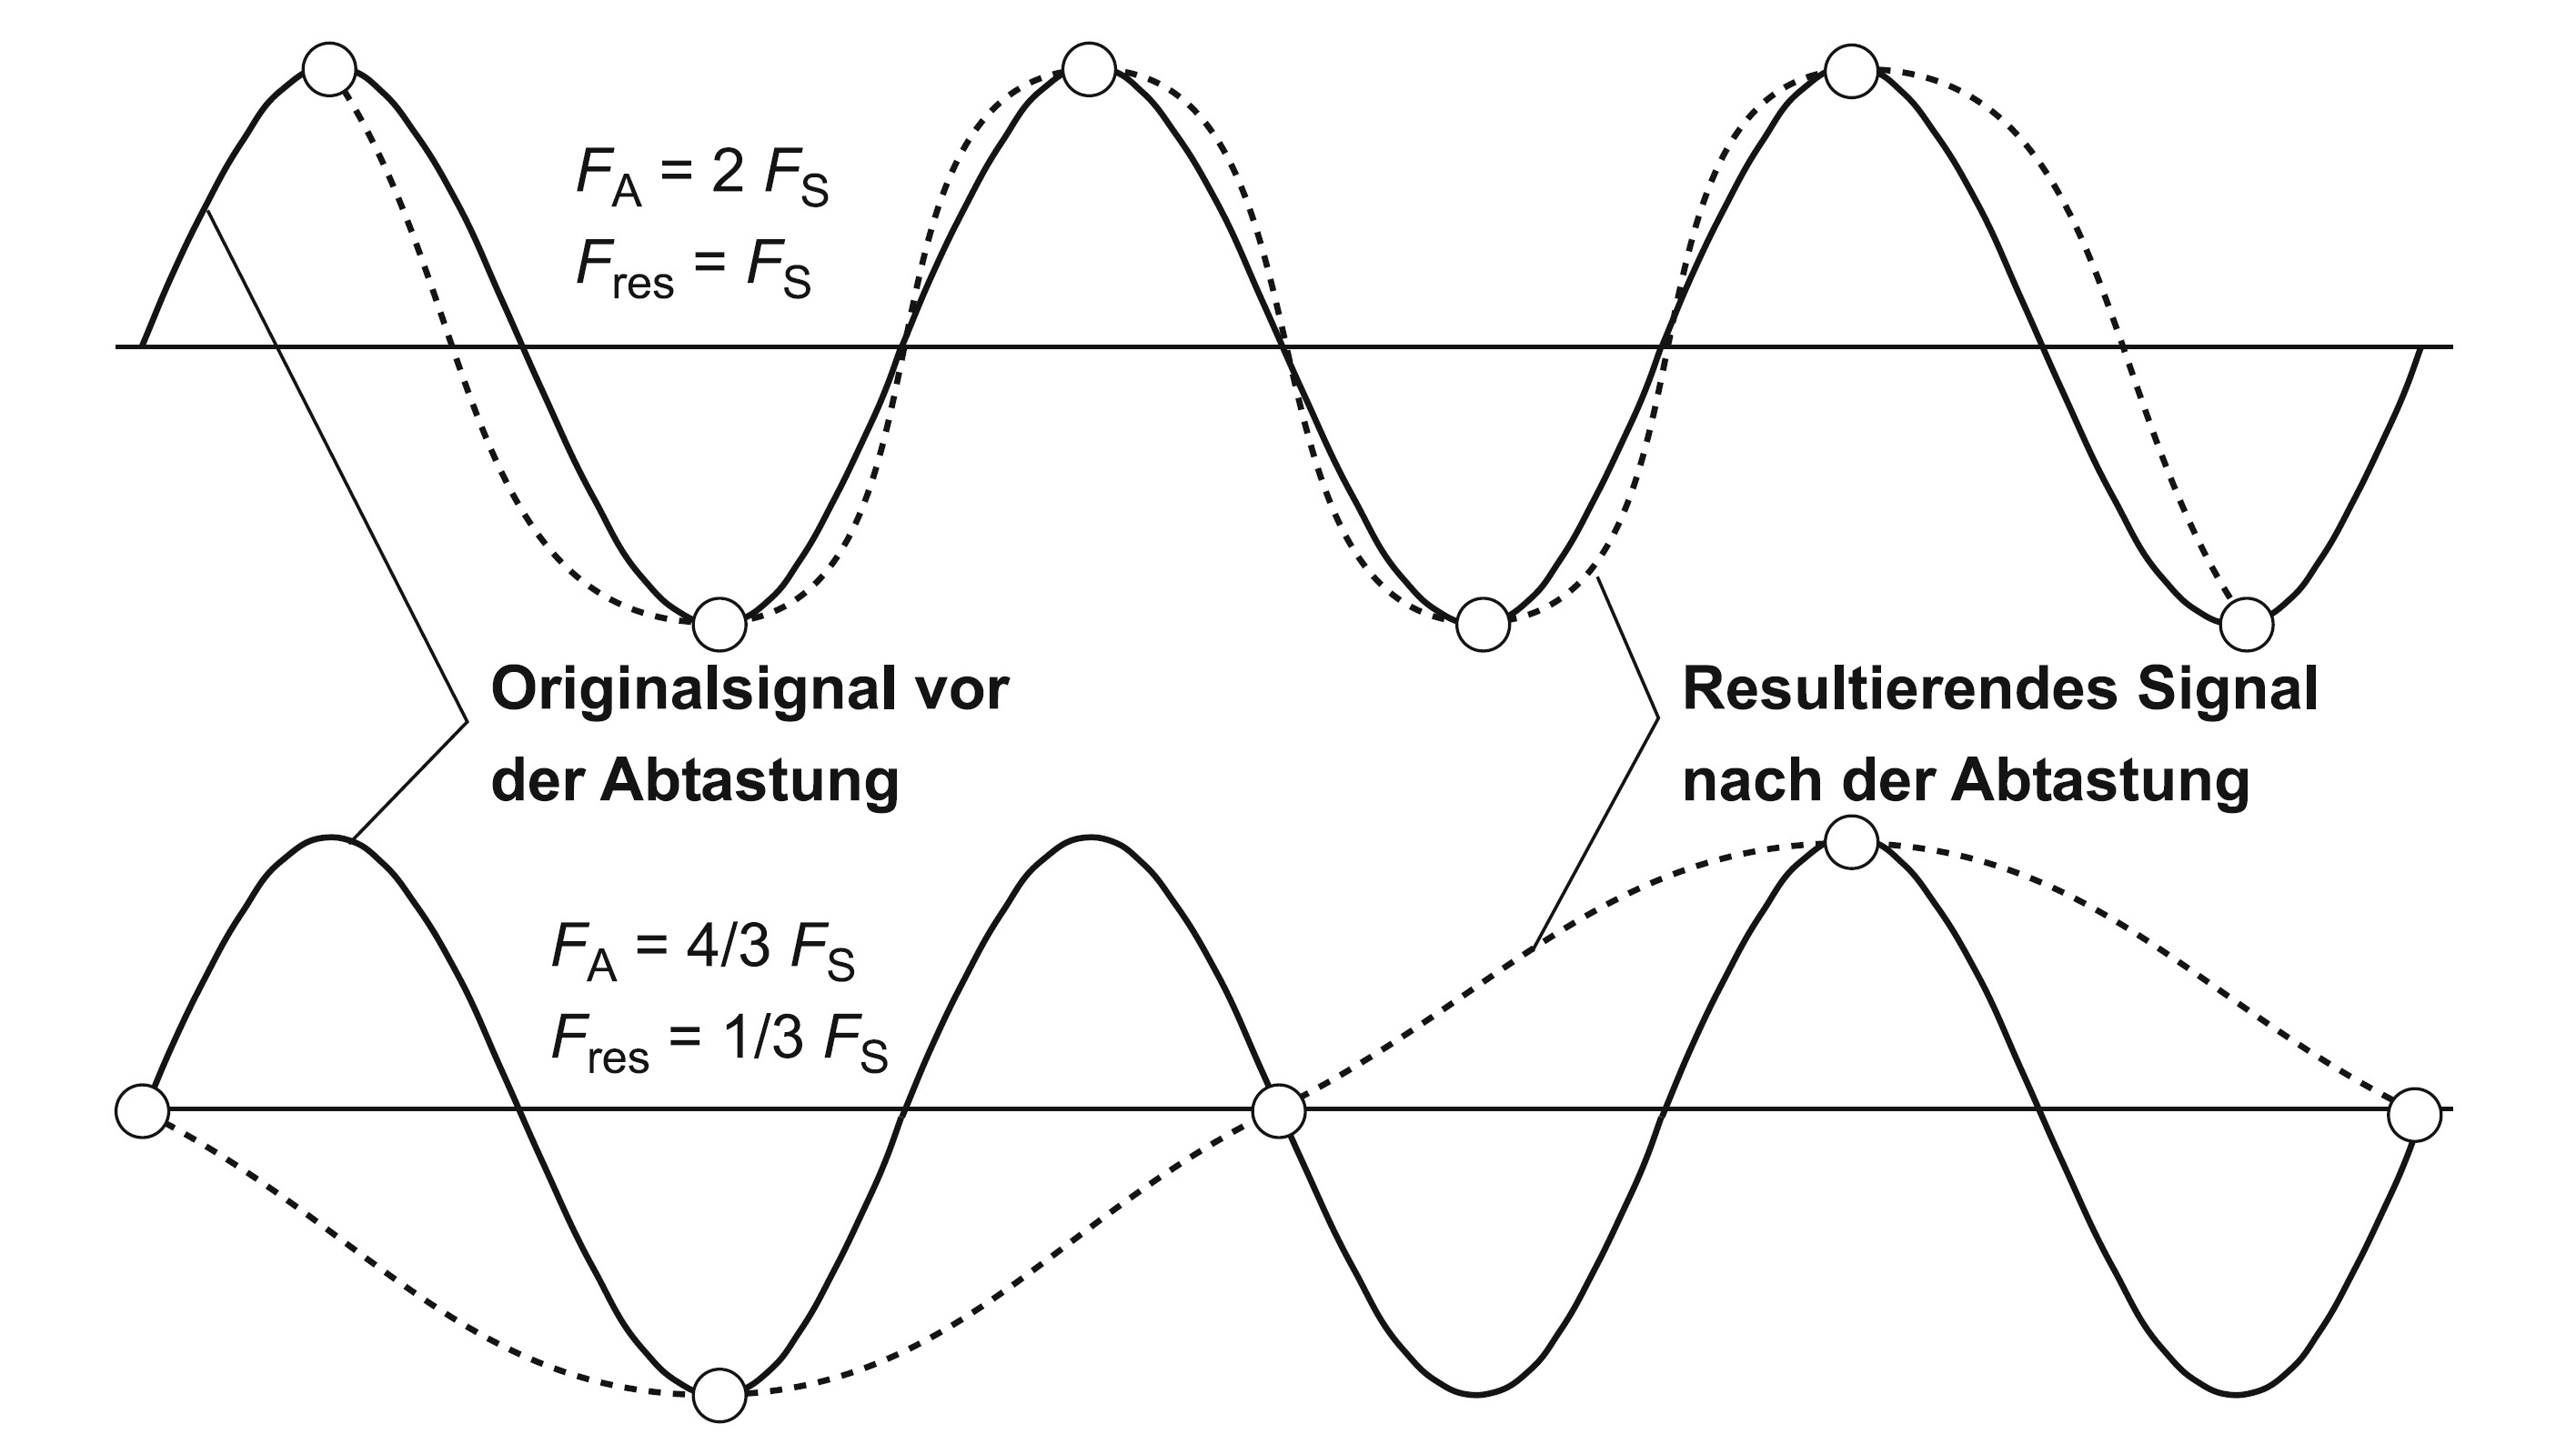
\includegraphics[width=0.8 \textwidth]{shannon.jpg}
	\caption[Vergleich zwischen Abtastung und Unterabtastung eines Signals]{Vergleich zwischen Abtastung und Unterabtastung eines Signals} \cite{stotzaudio}
	\label{fig:shannon}
\end{figure}

Empfehlenswert ist es also, das Shannon Theorem nur als absolute Untergrenze zu wählen und dazu zu neigen die Abtastfrequenz noch deutlich höher als das zweifache und maximal zu messende Signal zu bestimmen.\cite{stotzaudio} Im Audiobereich wird häufig mit 44,1 kHz oder mit 48 kHz abgetastet und somit das Shannon-Theorem eingehalten, da der Hörbereich des menschlichen Ohrs, welcher in Abbildung~\ref{fig:audiospektrum} illustriert wurde, bei 20 kHz endet. \cite{masteraudio}


\section{Einführung in die Übertagungstechnik}
\label{subsec:uebertragung}
In diesem Kapitel werden die Grundlagen der modernen Übertragungstechnik als Basis für die weiteren Ausführungen erklärt. Zunächst soll der generelle Aufbau eines Übertragungssystems erläutert werden, um anschließend einige gängige digitale Modulationsarten vorzustellen. Hierbei liegt der Fokus besonders auf der Heranführung an die \gls{acr:QAM}-Modulation, welche in der später diskutierten Dream-Software Verwendung findet. Der letzte Abschnitt beschäftigt sich mit den Themen der Bandbreitennutzung und des Mehrkanalzugriffs. Hier werden die aus der Mobilfunktechnik bekannten Begriffe \gls{acr:TDM}, \gls{acr:SDM} und \gls{acr:FDM} eingeführt und beschrieben. Ein besonderes Augenmerk liegt hier auf dem \gls{acr:OFDM}, einer weiterentwickelten Form des \gls{acr:FDM}. Zuletzt wird der zentrale Baustein der digitalen Signalverarbeitung in dieser Abschlussarbeit erläutert, das sogenannte \gls{acr:DRM}.

\subsection{Übertragungssystem}
\label{subsec:aufbauueber}

Ein Übertragungssystem ergibt sich vereinfacht dargestellt aus fünf verschiedenen Komponenten. In Abbildung~\ref{fig:komsystem} ist eine Skizze eines solchen Übertragungssystems zu sehen. Zunächst ist eine Quelle vonnöten, welche ein zeitkontinuierliches Signal (z.B. Sprache, Musik, Bilddaten, analoge Messwerte) oder ein zeitdiskretes Signal (z.B. Buchstaben, Datensequenzen, abgetastete analoge Signale) zur Verfügung stellt. Die Informationsquelle (information source) übergibt die Nachricht (message) dem Sender (transmitter). Der Sender übernimmt im System die Aufgabe, die Informationsquelle in ein für die Übertragung geeignetes Format umzuwandeln. Dieses muss auf den später zur Weiterleitung des Signals genutzten Kanal abgestimmt werden, welcher dann das entsprechende Sendesignal (signal) für den Kanal (channel) generiert. Im Kanal addiert sich, falls vorhanden, das Signal einer Störquelle (noise source) hinzu, sodass sich das Empfangssignal (received signal) am Empfänger (receiver) ergibt. Dabei gilt es darauf zu achten, den zur Verfügung stehenden Kanal und seine Eigenschaften möglichst effizient zu nutzen und die Störquelle zu minimieren. Sendekanäle sind physikalischer Natur und allgemein fehlerbehaftet. Es wird zwischen drahtlosen Kanälen (elektromagnetisch, akustisch, optisch) und drahtgebundenen Kanälen (Kupferleitungen, Glasfaserkabel) unterschieden. Im Anschluss generiert der Empfänger daraus dann die empfangene Nachricht (received message) und leitet jene schließlich der Informationssenke (destination) weiter. In Anbetracht ihrer Anwendung werden diese einzelnen Blöcke des Kommunikationsmodells in weitere Komponenten zerlegt und somit weiter spezialisiert.\cite{NT}

\begin{figure}[H]
	\centering
	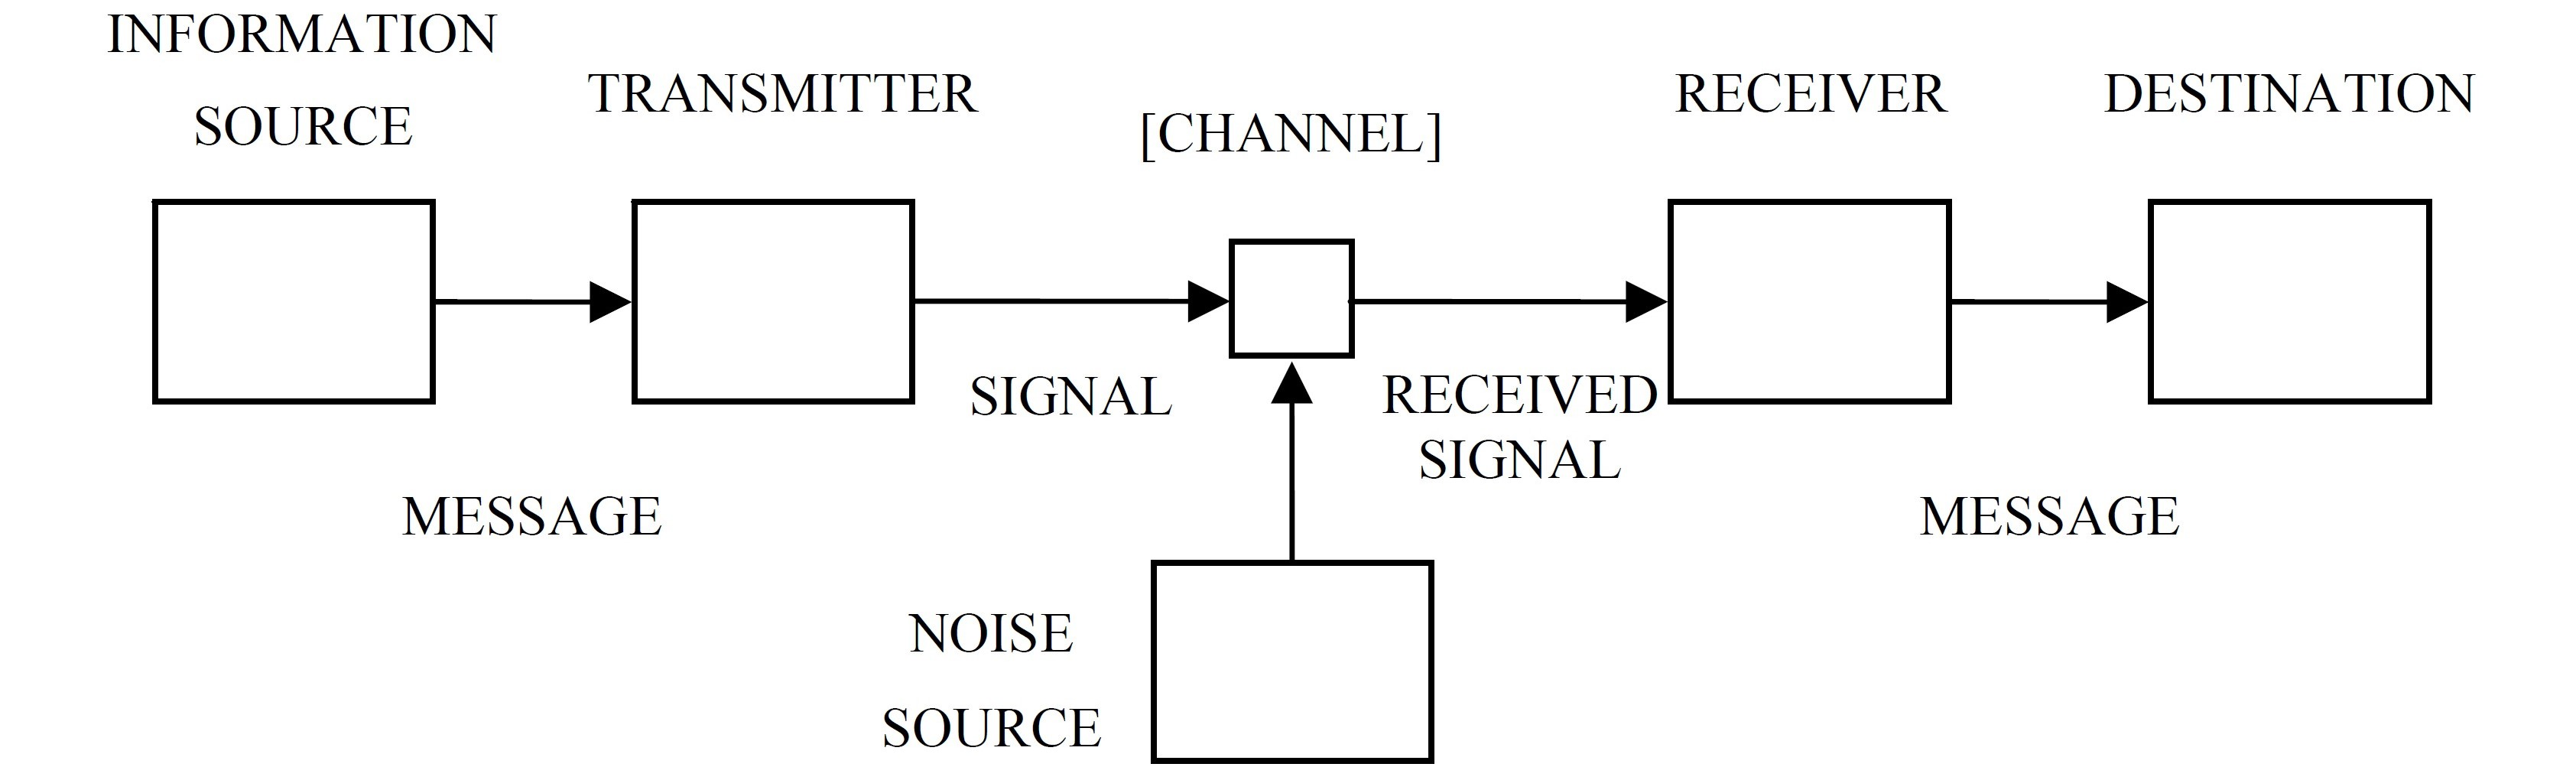
\includegraphics[width=1\textwidth]{komsystem.jpg}
	\caption[Nachrichtenübertragung nach Shannon]{Nachrichtenübertragung nach Shannon} 
	\cite{shannon}
	\label{fig:komsystem}
\end{figure}

Aufgrund der Thematik dieser Abschlussarbeit soll das Augenmerk nun auf ein drahtloses Übertragungssystem gelegt werden. Zur Projektierung eines solchen müssen zunächst der physikalische Kanal und die Signalform festgelegt werden. Da hierbei der optische Kanal als Übertragungsmedium dient, eignet sich \gls{acr:VLC} beispielsweise nicht für den Mobilfunk. Hier werden üblicherweise elektromagnetische Wellen in Megahertz bis Gigahertz Frequenzbereichen appliziert. Diese Wellen bestehen aus einem magnetischen Feld ($\vec{B}$) und einem elektrischen Feld ($\vec{E}$). Zudem breiten sich jene Felder orthogonal zueinander aus, wie in Abbildung ~\ref{fig:elektromag} veranschaulicht wird.\gls{online:elektromag} 

\begin{figure}[H]
	\centering
	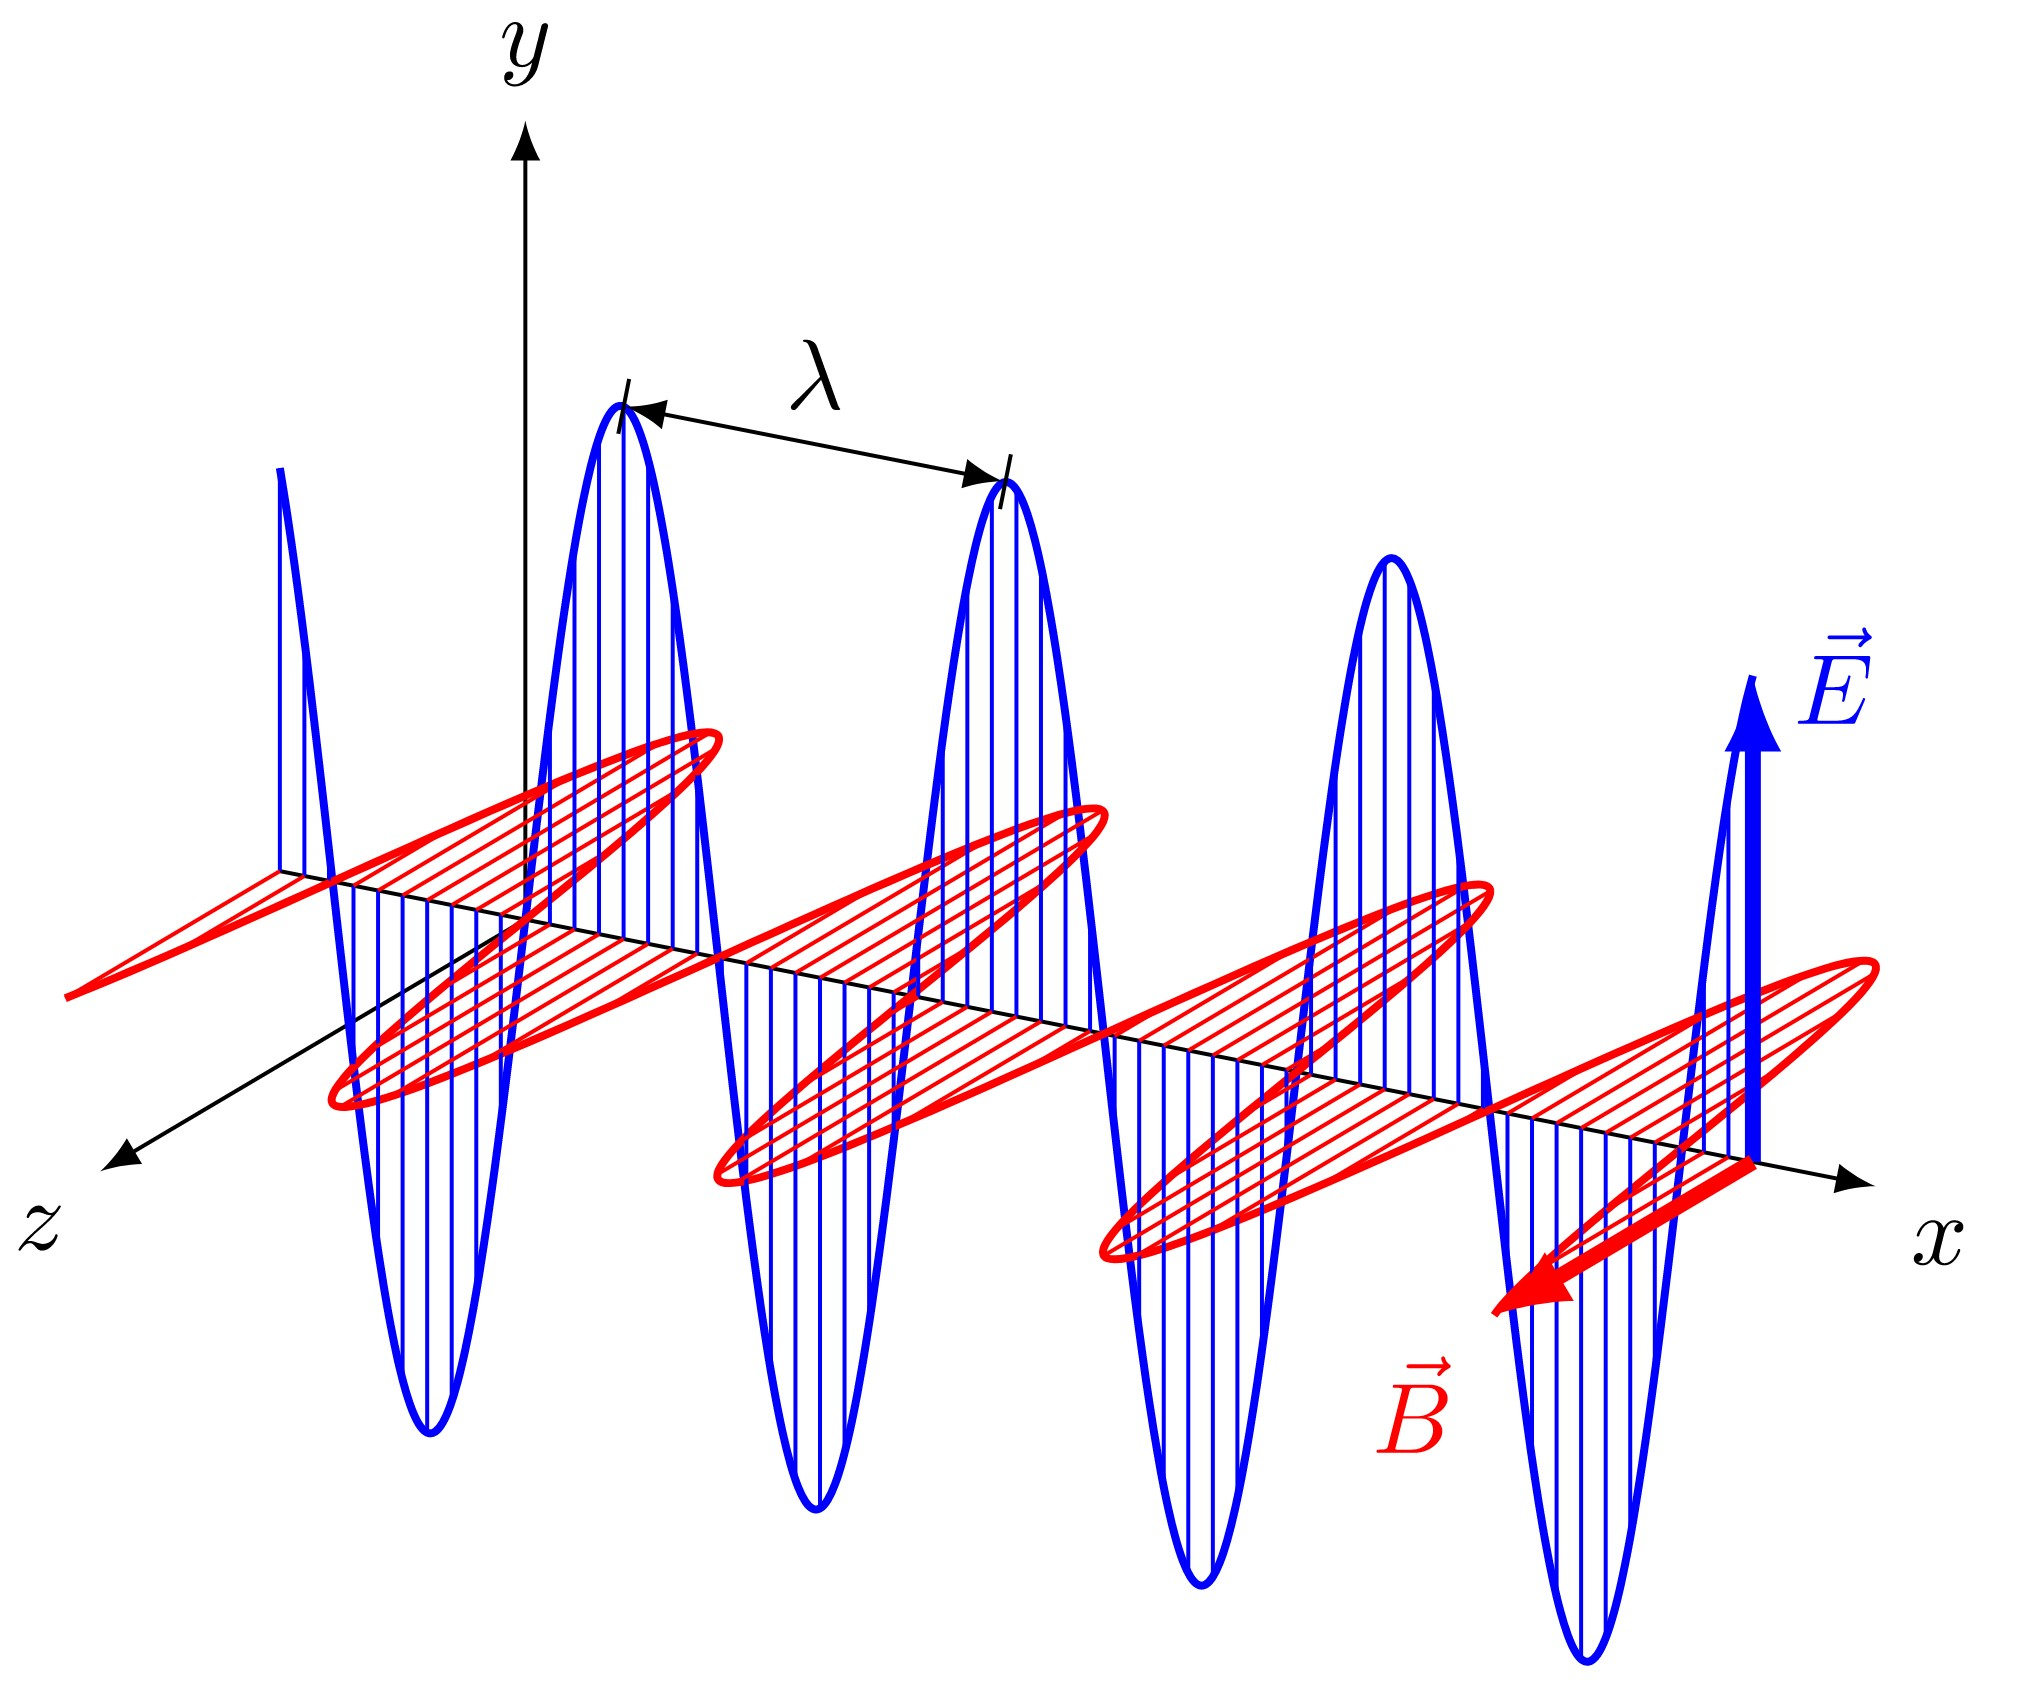
\includegraphics[width=0.8\textwidth]{elektromag.jpg}
	\caption[Ausbreitung einer elektromagnetischen Welle]{Ausbreitung einer elektromagnetischen Welle} 
	\gls{online:elektromag}
	\label{fig:elektromag}
\end{figure}
\begin{equation}
	\label{equ:lambda}
	\lambda = \frac{c}{f} 
\end{equation}

Eine solche Form von Wellen ist nicht an ein Ausbreitungsmedium gebunden, weshalb es sich auch im Vakuum (z.B. im Weltraum) ausbreiten kann. Diese Eigenschaft ermöglicht beispielsweise eine Satellitenkommunikation. Zur Erzeugung einer elektromagnetischen Welle wird zunächst eine hochfrequente Wechselspannung benötigt. Diese wird meist durch einen Quarzoszillator erzeugt. Damit sich die Welle nun ausbreiten kann, benötigt sie eine Antenne, von welcher sie sich ablösen kann.\cite{howwireless}\cite{NT} Um sich jedoch von einer Antenne zu lösen, muss die Wellenlänge $\lambda$  der elektromagnetische Welle ,welche in Formel~\ref{equ:lambda} dargestellt wurde, in die Größenordnung der Antennenabmessung kommen. Da ein Ton von 300Hz jedoch nach Formel~\ref{equ:lambda} eine mehrere Kilometer lange Antenne benötigen würde, muss mit Alternativen gearbeitet werden. Hieraus entsteht also die Bedingung, eine geeignete Trägerfrequenz zu bestimmen, um jener dann die zu versendende Information aufzumodulieren.\cite{hftech}\cite{hoeher} Zum Rundfunk existieren jedoch Alternativen. Beispielsweise Fernbedienungen nutzen als Signalform das Licht im Infrarot-Bereich, um Umschaltbefehle zu übertragen. Nach einem ähnlichen Prinzip funktioniert auch \gls{acr:VLC}. Die Schwierigkeit ist jedoch, dass der direkte Einfall des Lichts auf den Empfänger gegeben sein muss, weshalb die Reichweite dieser Form der Datenübertragung äußerst begrenzt ist.

\subsection{Trägermodulation und Konstellationsdiagramm}
\label{subsec:modulationsarten}

In Kapitel~\ref{subsec:aufbauueber} wurden die Struktur und die Komponenten näher ausgeführt, welche ein Übertragungssystem besitzt. Zudem wurden elektromagnetische Wellen eingeführt und die Bedeutung einer hochfrequenten Trägerfrequenz verdeutlicht. Hier soll nun die Funktionsweise einer Trägermodulation weiter ausgeführt werden.  

\begin{figure}[H]
	\centering
	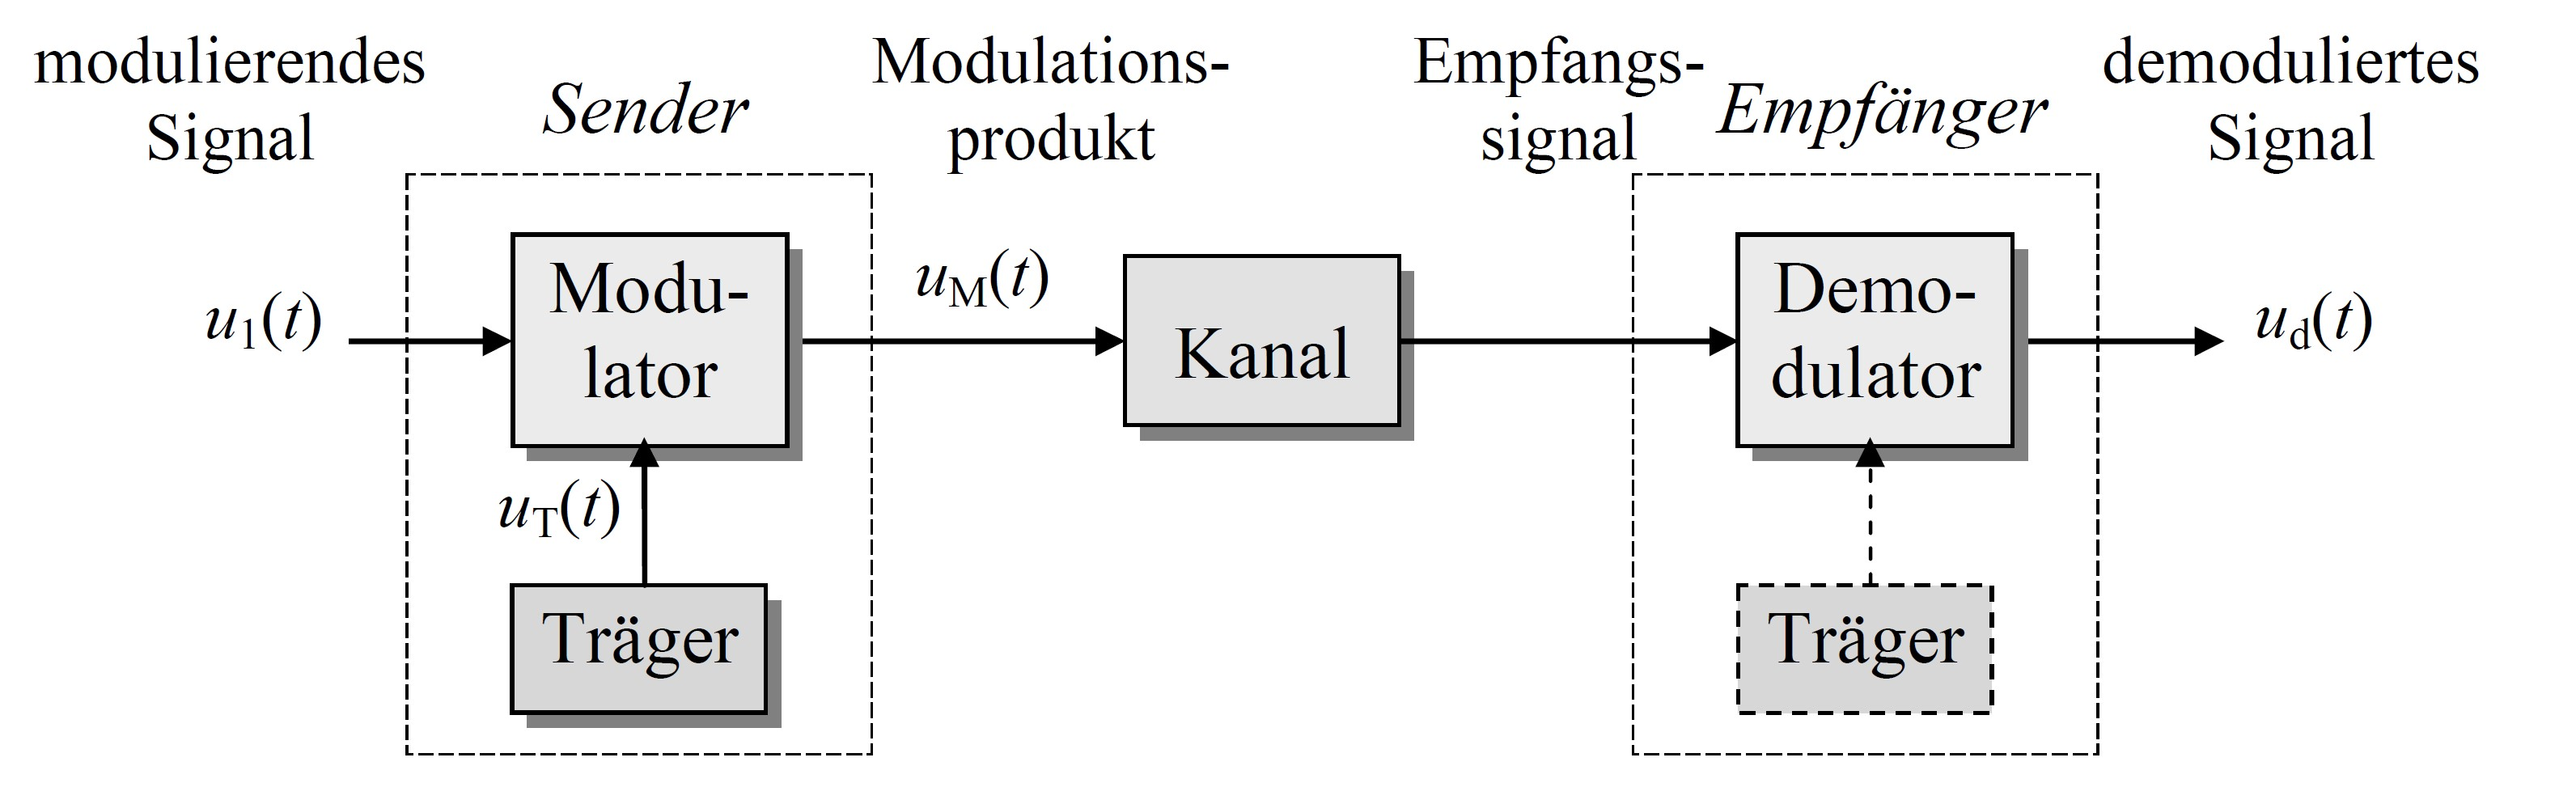
\includegraphics[width=1 \textwidth]{traegermod.jpg}
	\caption[Blockschaltbild einer Übertragung mit Trägermodulation]{Blockschaltbild einer Übertragung mit Trägermodulation} 
	\cite{NT}
	\label{fig:traeger}
\end{figure}
Liegt nun also ein Signal im Basisband vor, wobei es sich beispielsweise um ein Audiosignal als elektrische Spannung am Ausgang eines Mikrofons handeln könnte, wird es normalerweise in einen höheren Frequenzbereich verschoben um über eine größere Entfernung übertragen zu werden. Beim Basisband handelt es sich um den natürlichen Frequenzbereich eines Nutzsignals.\gls{online:basis} Radio-Rundfunk liefert ein Beispiel für eine solche Trägermodulation. Hierbei werden sich die drei variablen Parameter eines sinusförmigen Trägersignales zu eigen gemacht. Dabei handelt es sich um die Frequenz, Amplitude und Phase eines jenen. In Abhängigkeit der benutzten Verfahren ist die Rede von \gls{acr:AM}, \gls{acr:FM} oder \gls{acr:PM}.\cite{NT} Diese Theorie der Trägermodulation soll nun am Beispiel eines \gls{acr:AM}-Signals und eines \gls{acr:FM}-Signals veranschaulicht werden. 

\begin{figure}[H]
	\centering
	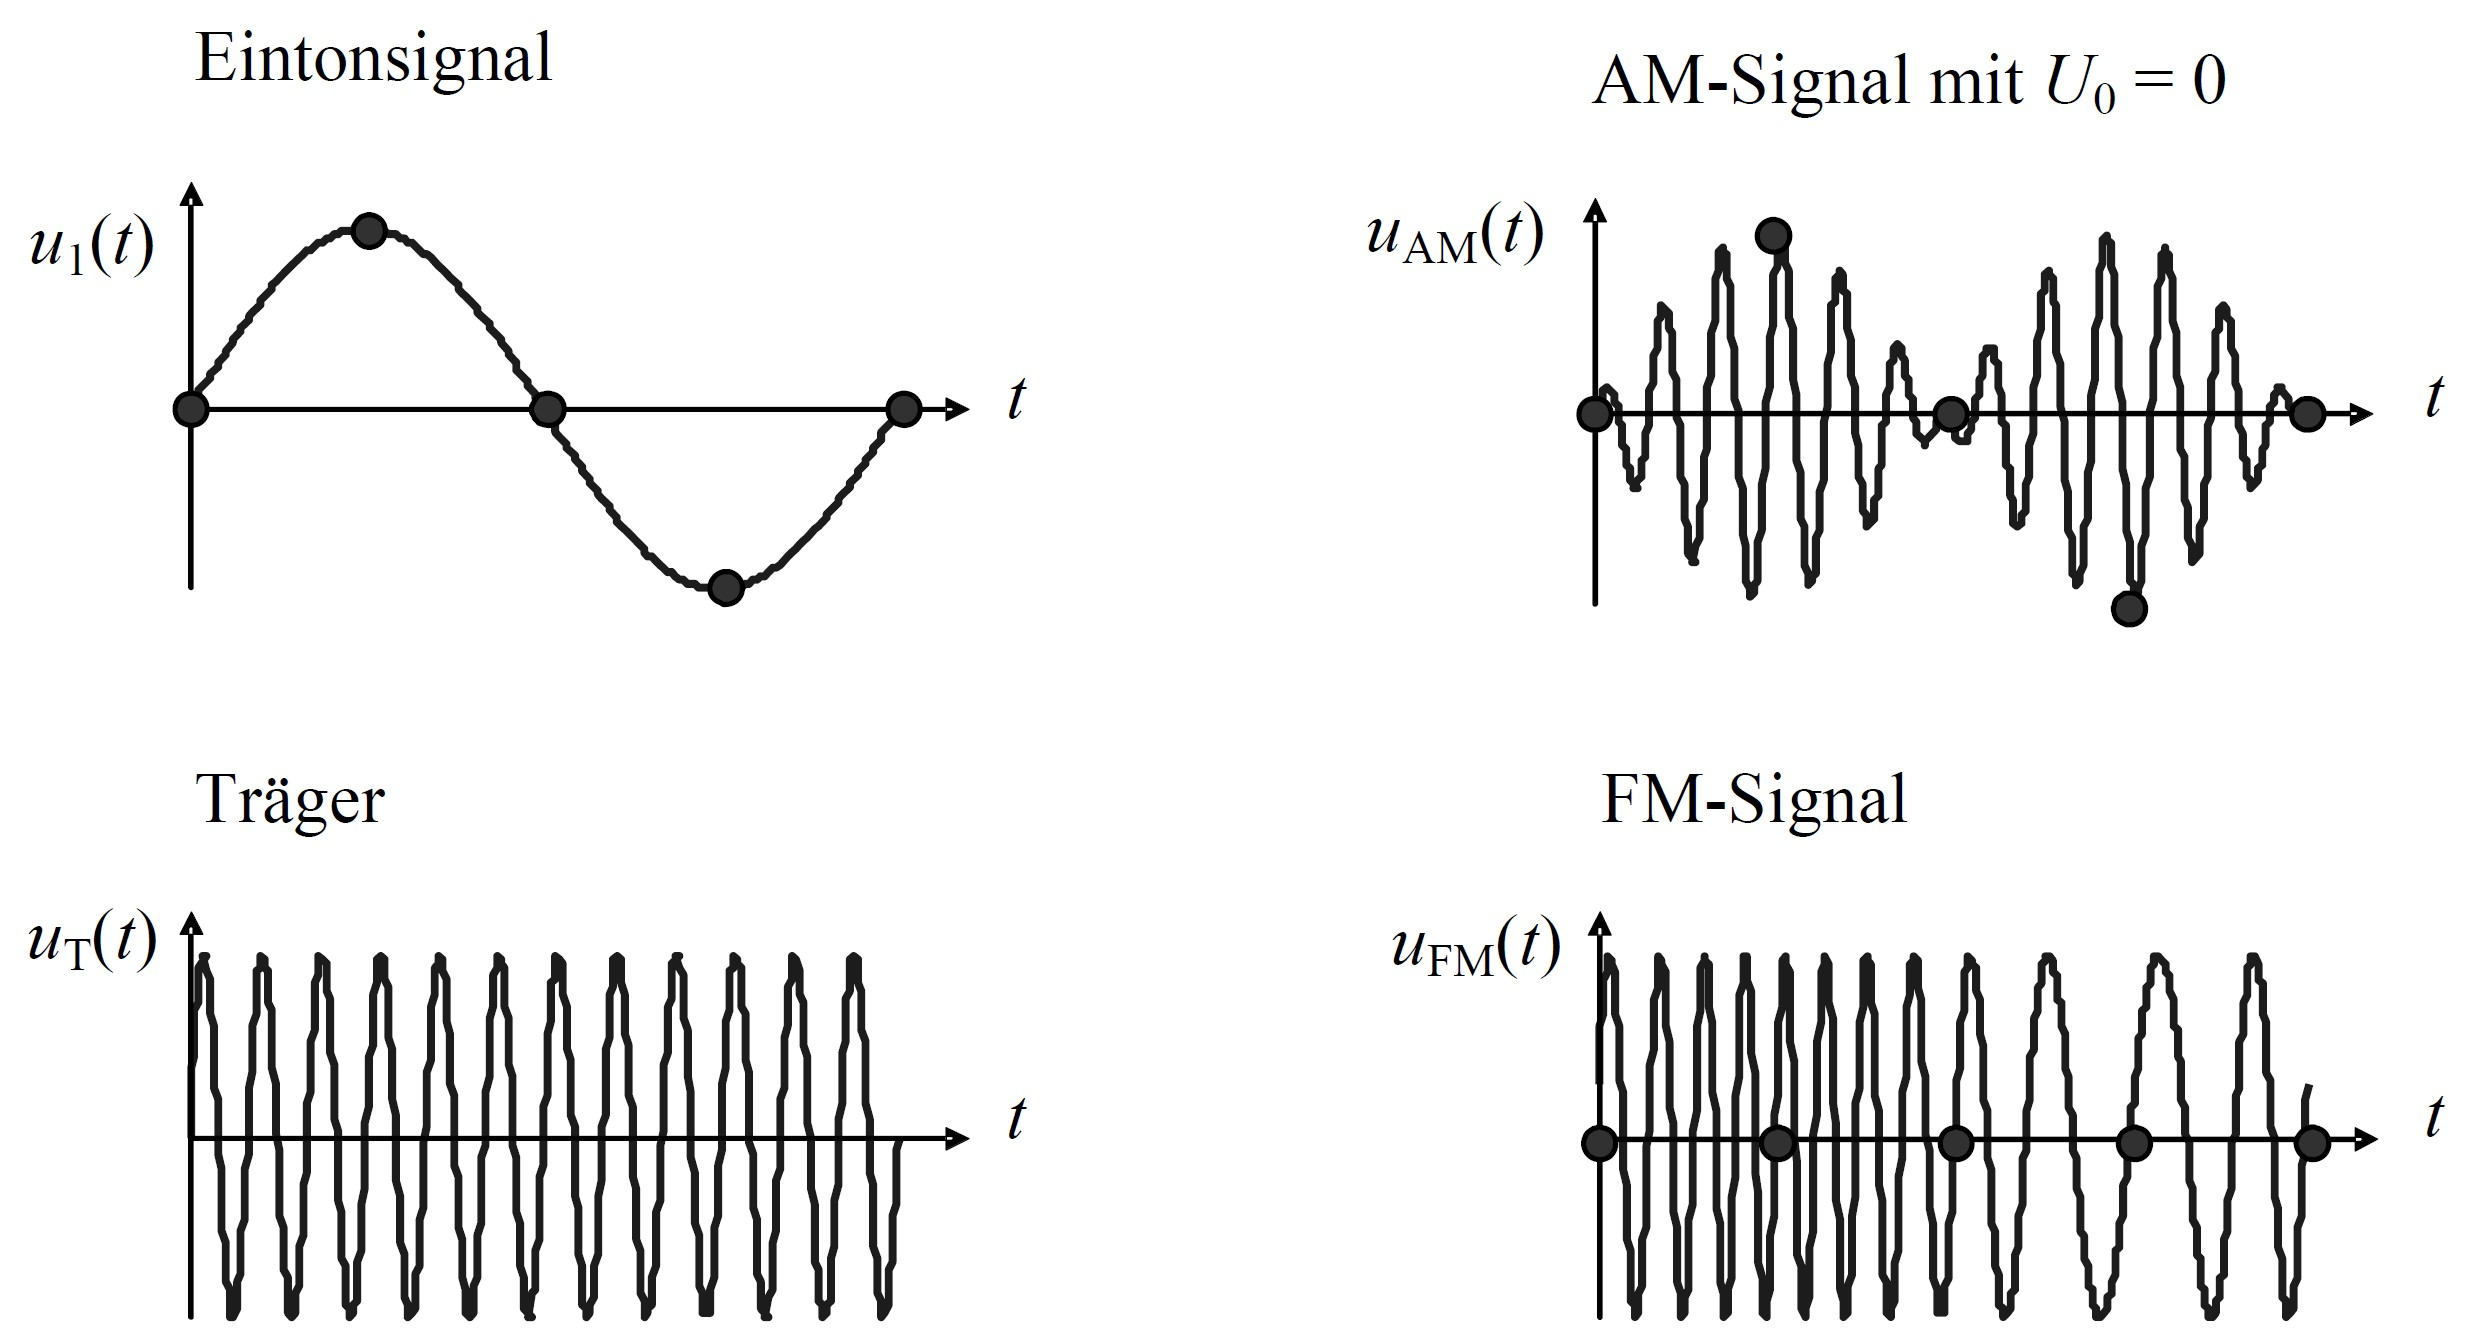
\includegraphics[width=0.85 \textwidth]{fmam.jpg}
	\caption[\gls{acr:AM}- und \gls{acr:FM}-Modulation eines Sinusträgers mit einem Eintonsignal]{\gls{acr:AM}- und \gls{acr:FM}-Modulation eines Sinusträgers mit einem Eintonsignal} 
	\cite{NT}
	\label{fig:fmam}
\end{figure}

Hierbei wird ein analoges Eingangssignal $u_1(t)$ verwendet. Es findet also keine Wandlung in ein digitales Signal statt. Bei der \gls{acr:AM} wird die sinusförmige Trägerfrequenz mithilfe eines Mischers auf das Signal multipliziert. Dabei gibt das Eintonsignal, wie in Abbildung~\ref{fig:fmam} die Amplitude der hochfrequenten Trägerfrequenz vor und bildet somit die Einhüllende Kurve. Durch diesen Vorgang erlangt das Signal eine adäquate Frequenz zur Ablösung einer Antenne.\cite{klostermeyerDigitaleModulation2001}\cite{hftech}

\begin{figure}[H]
	\centering
	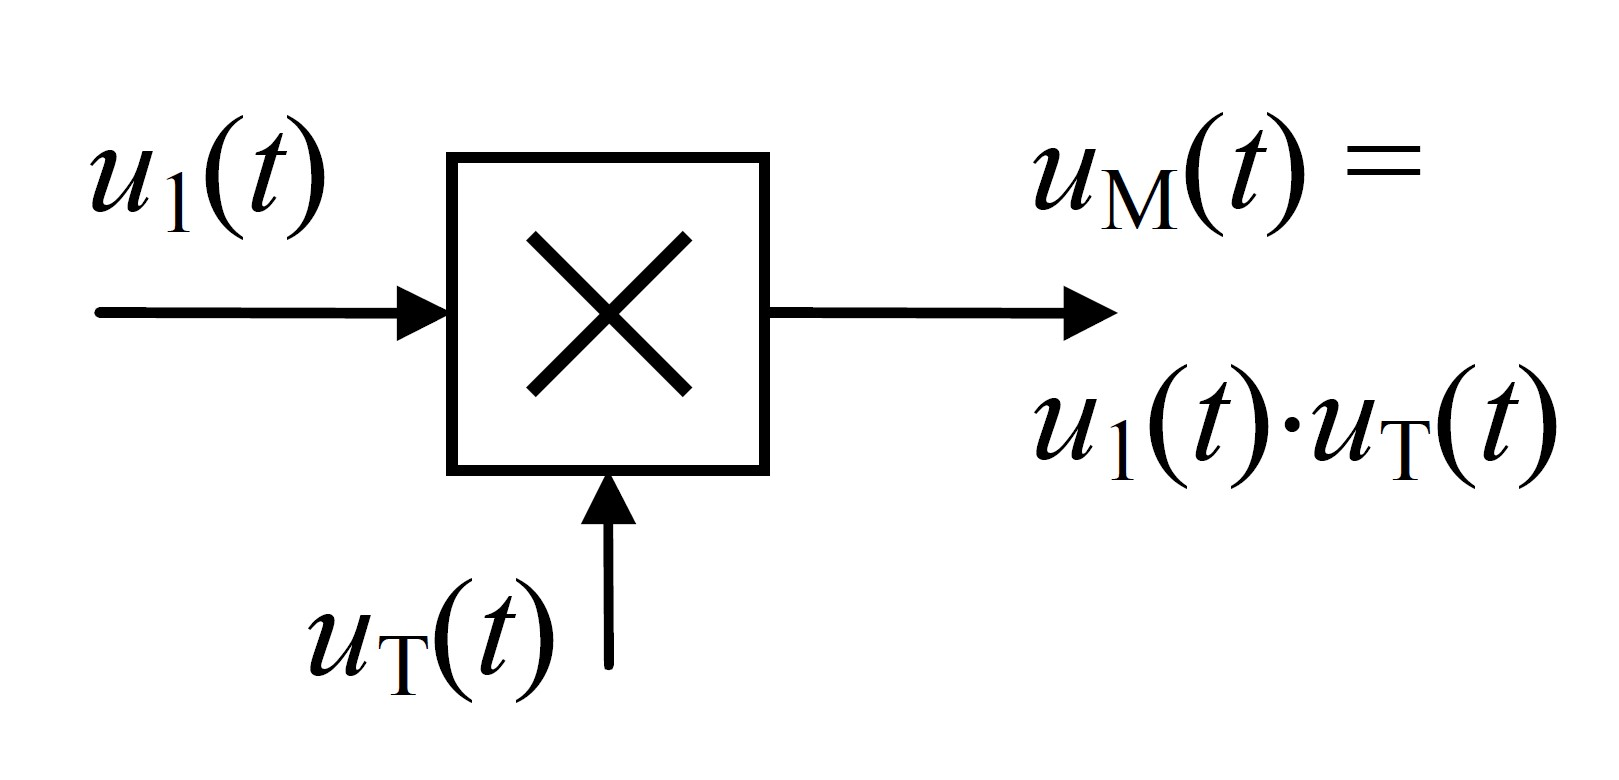
\includegraphics[width=0.3 \textwidth]{Mischer.jpg}
	\caption[Trägermultiplikation bei \gls{acr:AM}]{Trägermultiplikation bei \gls{acr:AM}} 
	\cite{NT}
	\label{fig:mischer}
\end{figure}

Bei Frequenzmodulation wiederum liegt die Information in der Frequenz und nicht in der Amplitude. Abbildung~\ref{fig:fmam} zeigt dies. Beim frequenzmodulierten Signal ändert sich lediglich die Trägerfrequenz, wodurch diese Art von Modulation additiven Störungen gegenüber deutlich resistenter ist, da keine so starke Amplitudenschwankungen auftreten.\cite{hoeher}


Zur Vertiefung des Basiswissen werden nun noch digitale Modulationsarten erläutert. Hierbei wird auch mit der Variation von Frequenz, Amplitude und Phase gearbeitet. Diese drei Grundmodulationsarten sind in ihrer zweiwertigen Form 2-\gls{acr:ASK}, 2-\gls{acr:FSK} und 2-\gls{acr:PSK} in Darstellung~\ref{fig:welle} veranschaulicht.

\begin{figure}[H]
	\centering
	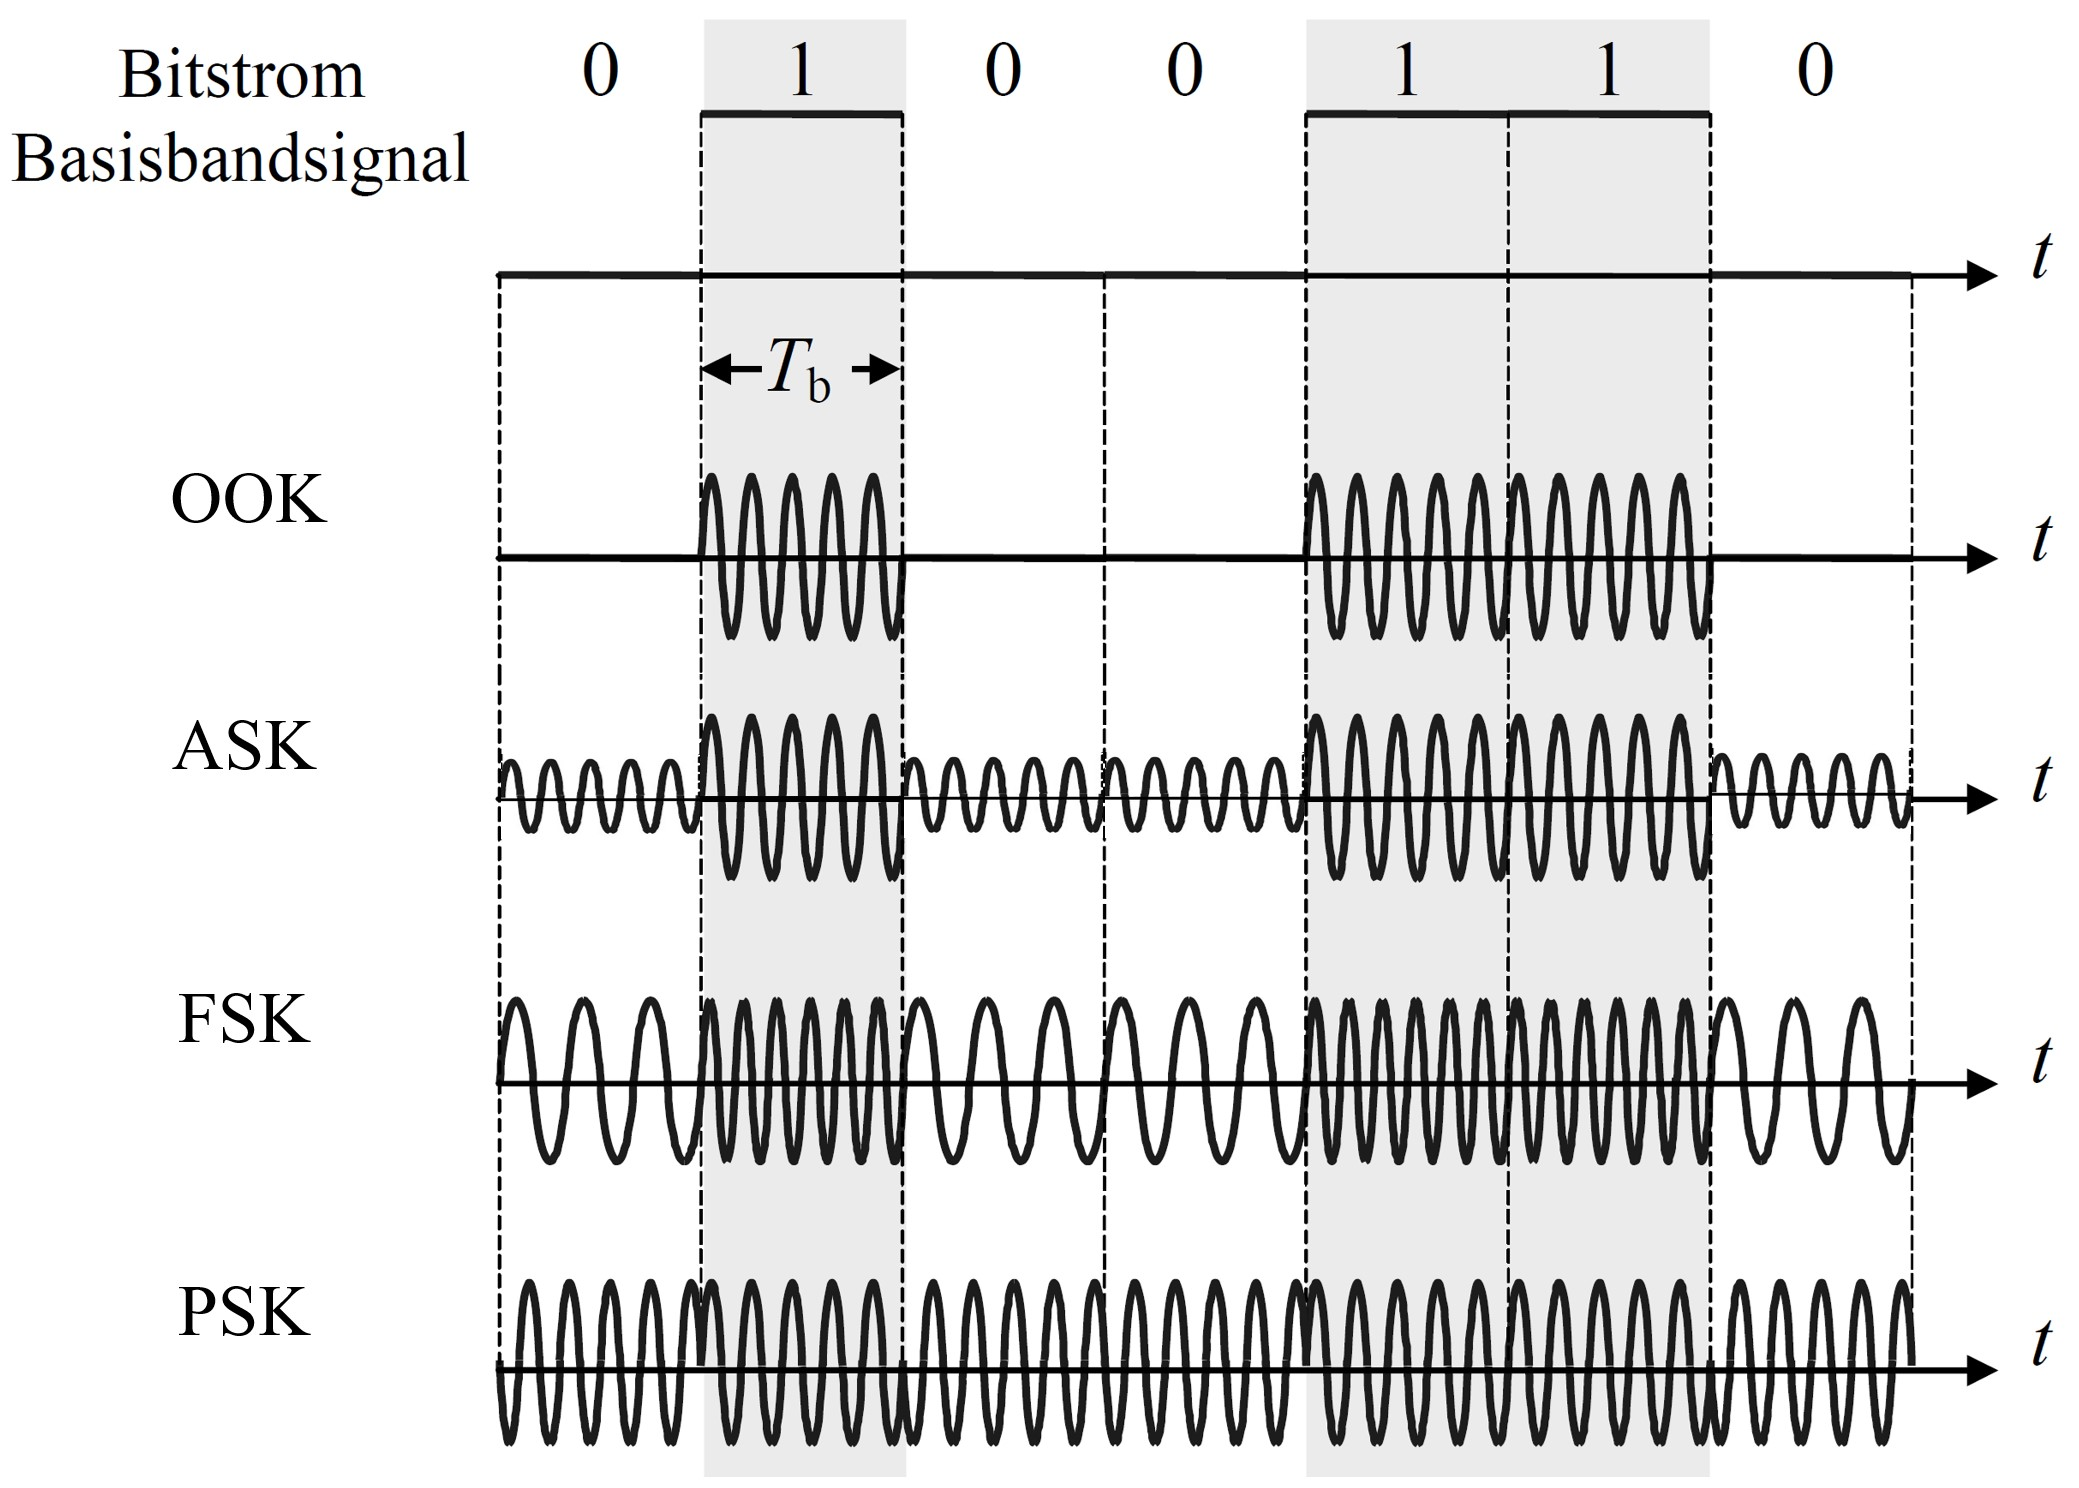
\includegraphics[width=0.9 \textwidth]{welle.jpg}
	\caption[Binäre Übertragung mit Sinusträger]{Binäre Übertragung mit Sinusträger} 
	\cite{NT}\gls{online:Eigen}
	\label{fig:welle}
\end{figure}

Hierbei wurde noch eine weitere Version der \gls{acr:AM}-Modulation illustriert. Diese nennt sich \gls{acr:OOK} und hat bei der Übertragung einer digitalen $"1"$ eine Amplitude und wird jedoch bei der Übertragung einer digitalen $"0"$ auf Null gesetzt. Da unter diesen Voraussetzungen nicht ermittelt werden kann wann die Übertragung endet, wird in der Praxis bei der \gls{acr:AM}-Modulation ein Zwischenwert mit z.B. halber Amplitude zum Senden einer digitalen $"0"$ verwendet. Ein übertragenes Bit entspricht bei zweiwertigen Modulationen einem Symbol. Modernere Kommunikationssysteme verwenden mittlerweile jedoch höherwertige Modulationsarten die es ermöglichen mehrere Bits pro Symbol zu übertragen. Bei zwei Bit werden hierbei vier Zustände benötigt. Daraus entstehen dann Erweiterungen der genannten Modulationsarten, welche z.B. als 4-\gls{acr:ASK}, 4-\gls{acr:FSK} und 4-\gls{acr:PSK} bezeichnet werden. Oft wird die Ziffer Vier auch mit dem Buchstaben $"Q"$ für Quadratur ersetzt.\cite{howwireless}\cite{butlerWirelessNetworkingDeveloping2013} Bei einer \gls{acr:QAM} wird beispielsweise eine Kombination zweier Modulationsarten verwendet. Dabei werden sowohl die Amplituden- als auch Phasenmanipulation benutzt, um Informationen zu modulieren. 

Da im Zuge dieser Abschlussarbeit größtenteils mit einer \gls{acr:QAM}-Modulaton gearbeitet wurde, wird diese näher erläutert. Um jedoch ein besseres Verständnis für den Aufbau einer solchen Modulation zu erlangen, muss der Begriff des Konstellationsdiagramms eingeführt werden. Dies soll am Beispiel einer \gls{acr:QPSK} veranschaulicht werden. Modulierte Wellen, sind sinusförmig und wie folgt definiert. 

\begin{equation}
	\label{equ:qpsk}
	s_{i}(t) = A \cdot cos(\omega \cdot t+\varphi_{0}+\varphi_{i})
\end{equation}

Dabei steht die Variable $A$ für eine, bei der \gls{acr:QPSK}, konstante Amplitude. Die variable $\varphi_{0}$ beschriebt zusätzlich die Phase des Referenzsignals. Und $\varphi_{i}$ beschreibt zuletzt die Phasenverschiebung zwischen den einzelnen Symbolen. Zudem ergibt sich die in Formel~\ref{equ:qpsk} genannte Kreisfrequenz $\omega$ aus:

\begin{equation}
	\label{equ:omega}
	\omega = 2 \cdot \pi \cdot f
\end{equation}
Da sich durch die konstante Amplitude die Symbole auf einem Kreis befinden, wird zur Maximierung des Abstandes bei der \gls{acr:QPSK} eine Verschiebung um 90$^\circ$ vorgenommen. Tabelle~\ref{tab:qpsk} gibt Information über die verschiedenen Phasenlagen die von $i$ angenommen werden können.\gls{online:quint}
\begin{table}[htb]
\centering
		\begin{tabular}[h]{ccc}	
			\toprule
			Funktion & $\varphi_{i}$& $\varphi_{0}$ \\
			\midrule
			$s_{1}(t)$ & $0^\circ$ & $45^\circ$ \\
			$s_{2}(t)$ & $90^\circ$ & $45^\circ$\\
			$s_{3}(t)$ & $180^\circ$ & $45^\circ$\\
			$s_{4}(t)$ & $270^\circ$& $45^\circ$ \\
			\bottomrule
		\end{tabular}
		\caption{Phasenlagen bei der \gls{acr:QPSK}}
		\label{tab:qpsk}
\end{table}

Ein Konstellationsdiagramm veranschaulicht die verschiedenen Symbole, mit Betrag und Phasenlage, im komplexen Raum. Zur Verringerung der Bitfehler wird hier der Gray Code für die Zuordnung von Bits gewählt. Dies hat zu Folge, dass wenn ein Symbol fälschlicherweise dem benachbarten Symbol zugeordnet wird, nur ein Bit fehlerhaft ist. Bei einer Binären Codierung könnte beispielsweise die 00 der 11 zugeordnet werden, wodurch zwei Bit in einem Symbol inkorrekt wären. Die Anzahl der differierenden Bit zweier benachbarter Symbole wird auch Hamming Abstand genannt.\gls{online:ham}

\begin{figure}[H]
	\centering
	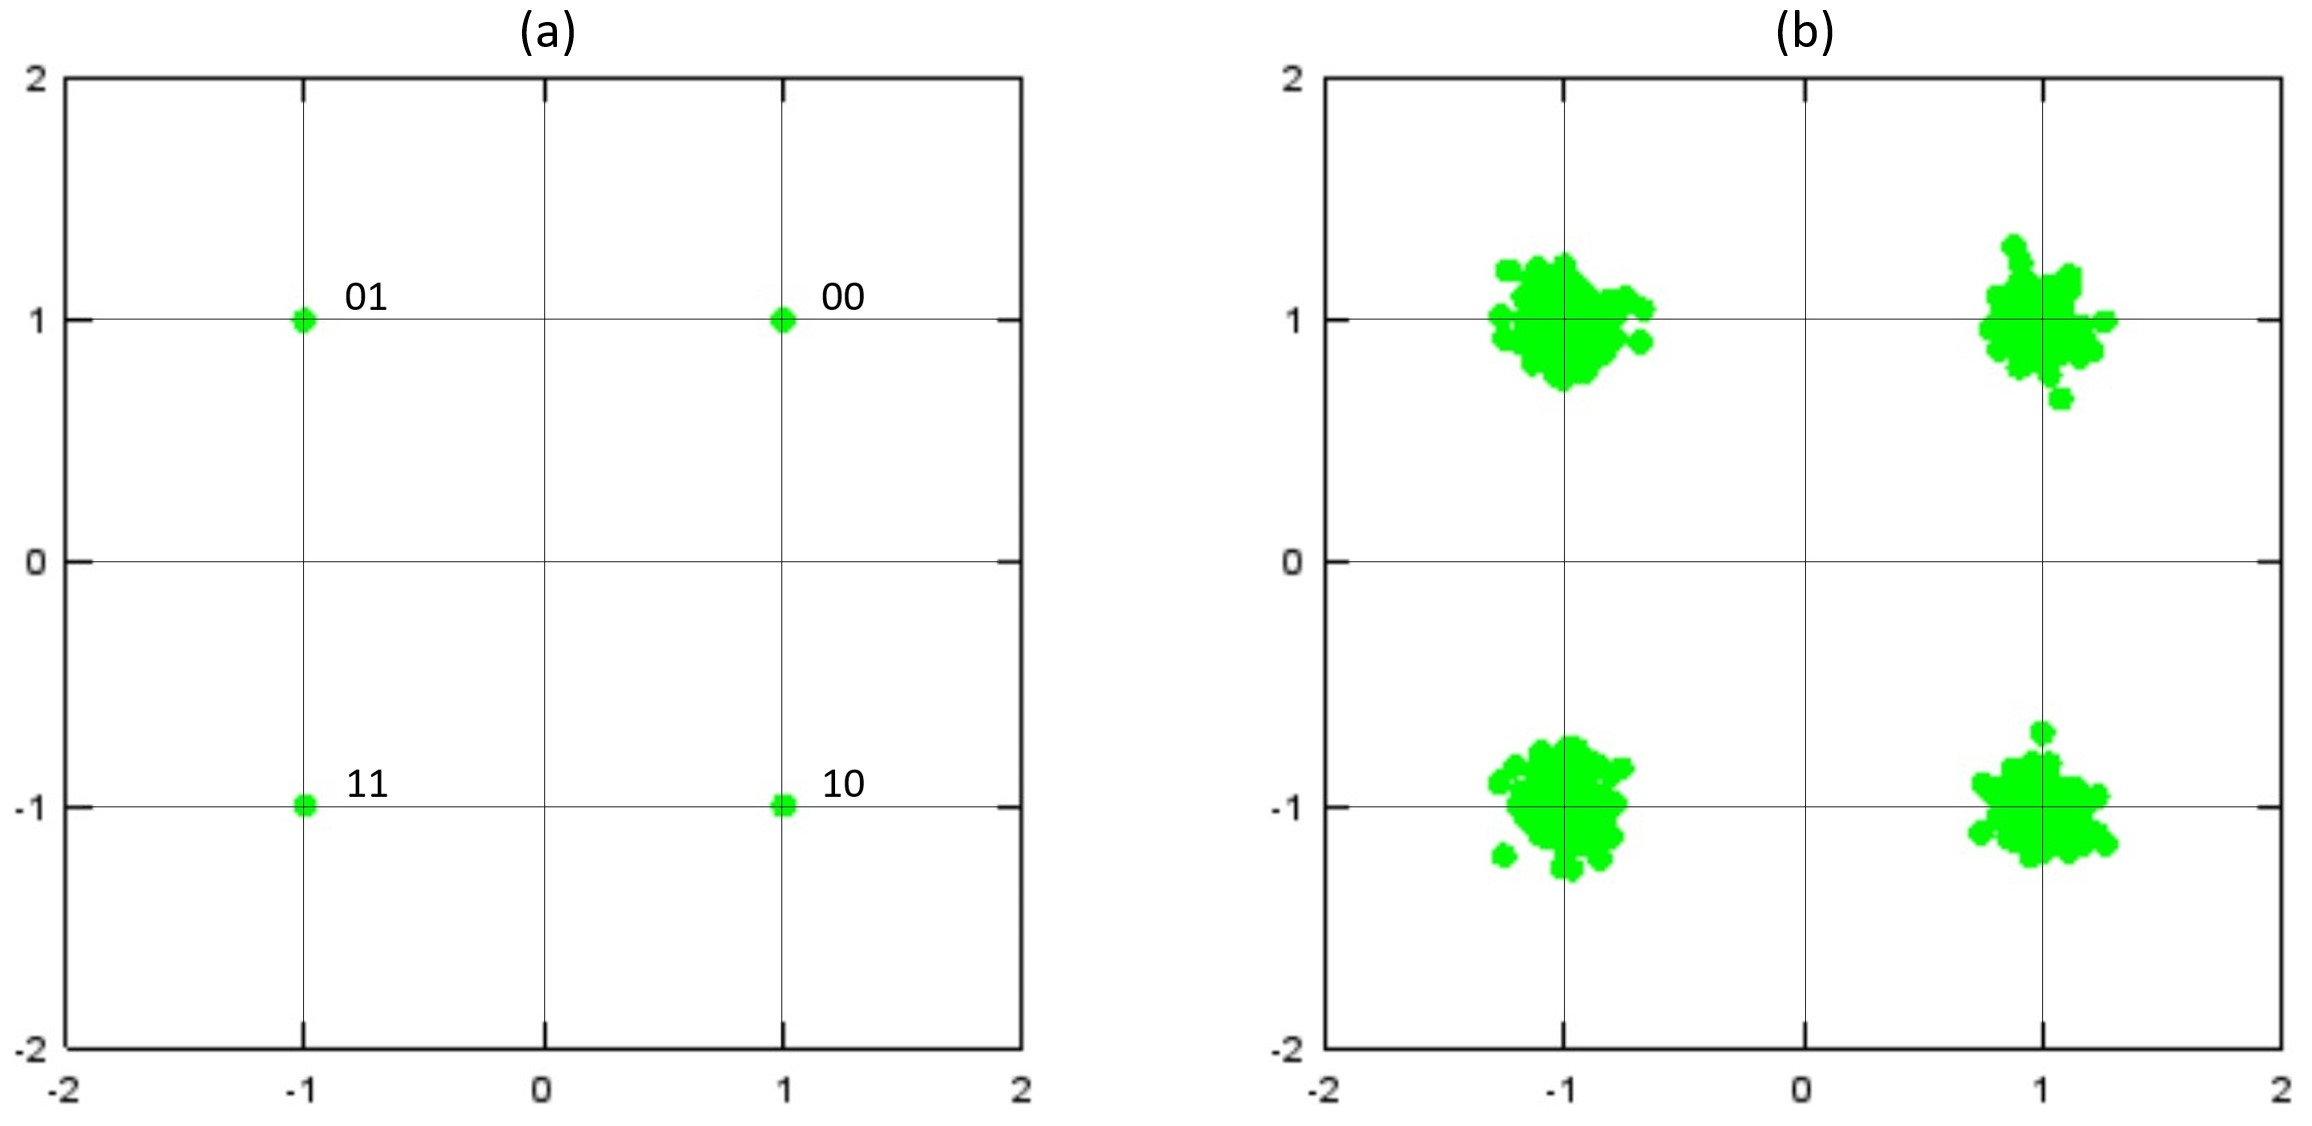
\includegraphics[width=0.9 \textwidth]{konstqpsk.jpg}
	\caption[Konstellationsdiagramm mit $\varphi_{0}$=$45^\circ$ im komplexen Raum]{Konstellationsdiagramm mit $\varphi_{0}$=45$^\circ$ im komplexen Raum} 
	\gls{online:konst}
	\label{fig:konstqpsk}
\end{figure}

In Abbildung~\ref{fig:konstqpsk} sind zwei Konstellationsdiagramme zu erkennen. Konstellationsdiagramm $(a)$ ist hierbei ein klares rauschfrei empfangenes Signal, $(b)$ hingegen wurde über einen verrauschten Kanal gesendet. Alle empfangenen Symbole häufen sich um die vier Symbolpunkte. Aufgrund des hier nur schwach verrauschten Kanals, können die Symbole noch problemlos zugeordnet werden. Bei einem sehr stark verrauschten Kanal jedoch, wäre diese Entscheidung unmöglich, wie in Abbildung~\ref{fig:verrauscht} zu sehen ist. Daher werden klare Entscheidungsgrenzen definiert, im gegeben Fall sind das die reelle und die imaginären Achse.\gls{online:quint}

\begin{figure}[H]
	\centering
	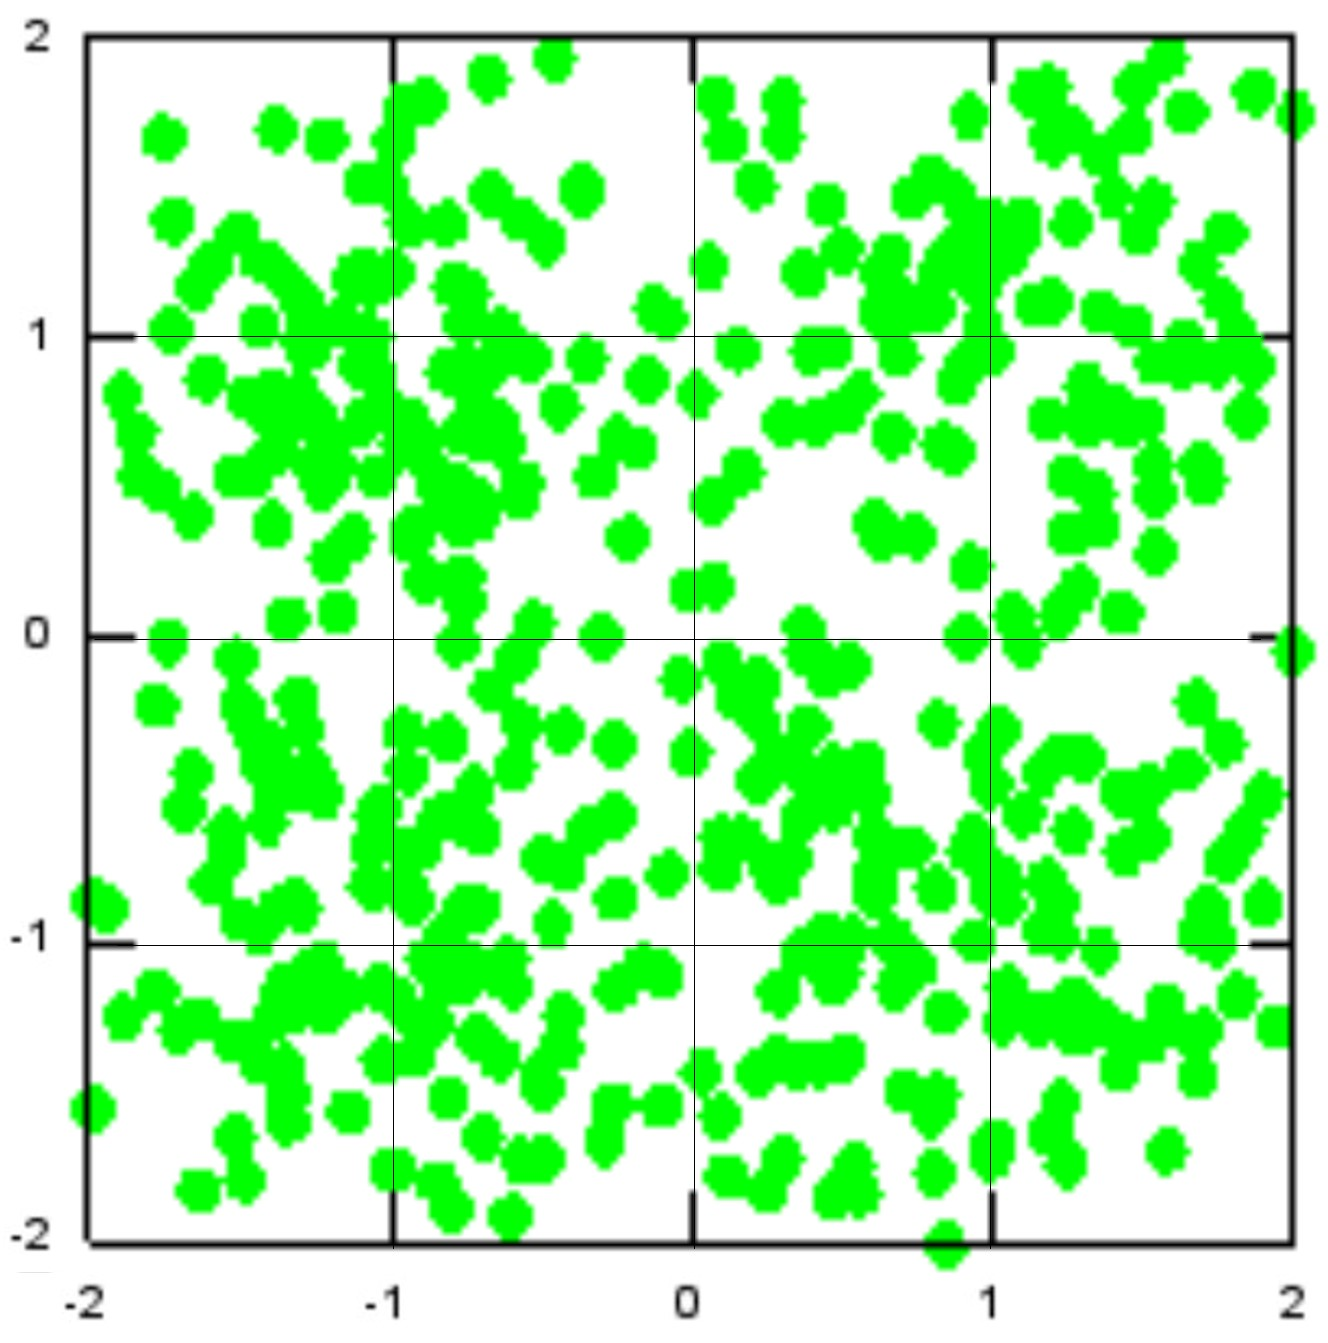
\includegraphics[width=0.42 \textwidth]{verrauscht.jpg}
	\caption[Konstellationsdiagramm mit $\varphi_{0}=45^\circ$ mit stark verrauschtem Kanal]{Konstellationsdiagramm mit $\varphi_{0}=45^\circ$ mit stark verrauschtem Kanal} 
	\gls{online:konst}
	\label{fig:verrauscht}
\end{figure}

Ein solches Vorgehen ist jedoch bei höherwertigen \gls{acr:PSK}-Modulationen nicht mehr sinnvoll, da die Symbolabstände immer geringer werden würden und die Übertragung somit störanfälliger wird. Durch die konstante Amplitude würden sich der Symbolabstand auf der Kreisbahn mit steigender Symbolzahl verringern. Sinnvoller ist es also die \gls{acr:QPSK} so zu erweitern, dass in der Wellengleichung nicht nur $\varphi_{i}$ variiert wird, sondern auch die Amplitude $A$. Durch diese Erweiterung kann die Bitrate enorm gesteigert werden. Exemplarisch hierfür sind die in Abbildung~\ref{fig:qam} gezeigten 16-\gls{acr:QAM} und die 64-\gls{acr:QAM} welche im Laufe dieser Abschlussarbeit noch Verwendung finden.

\begin{figure}[H]
	\centering
	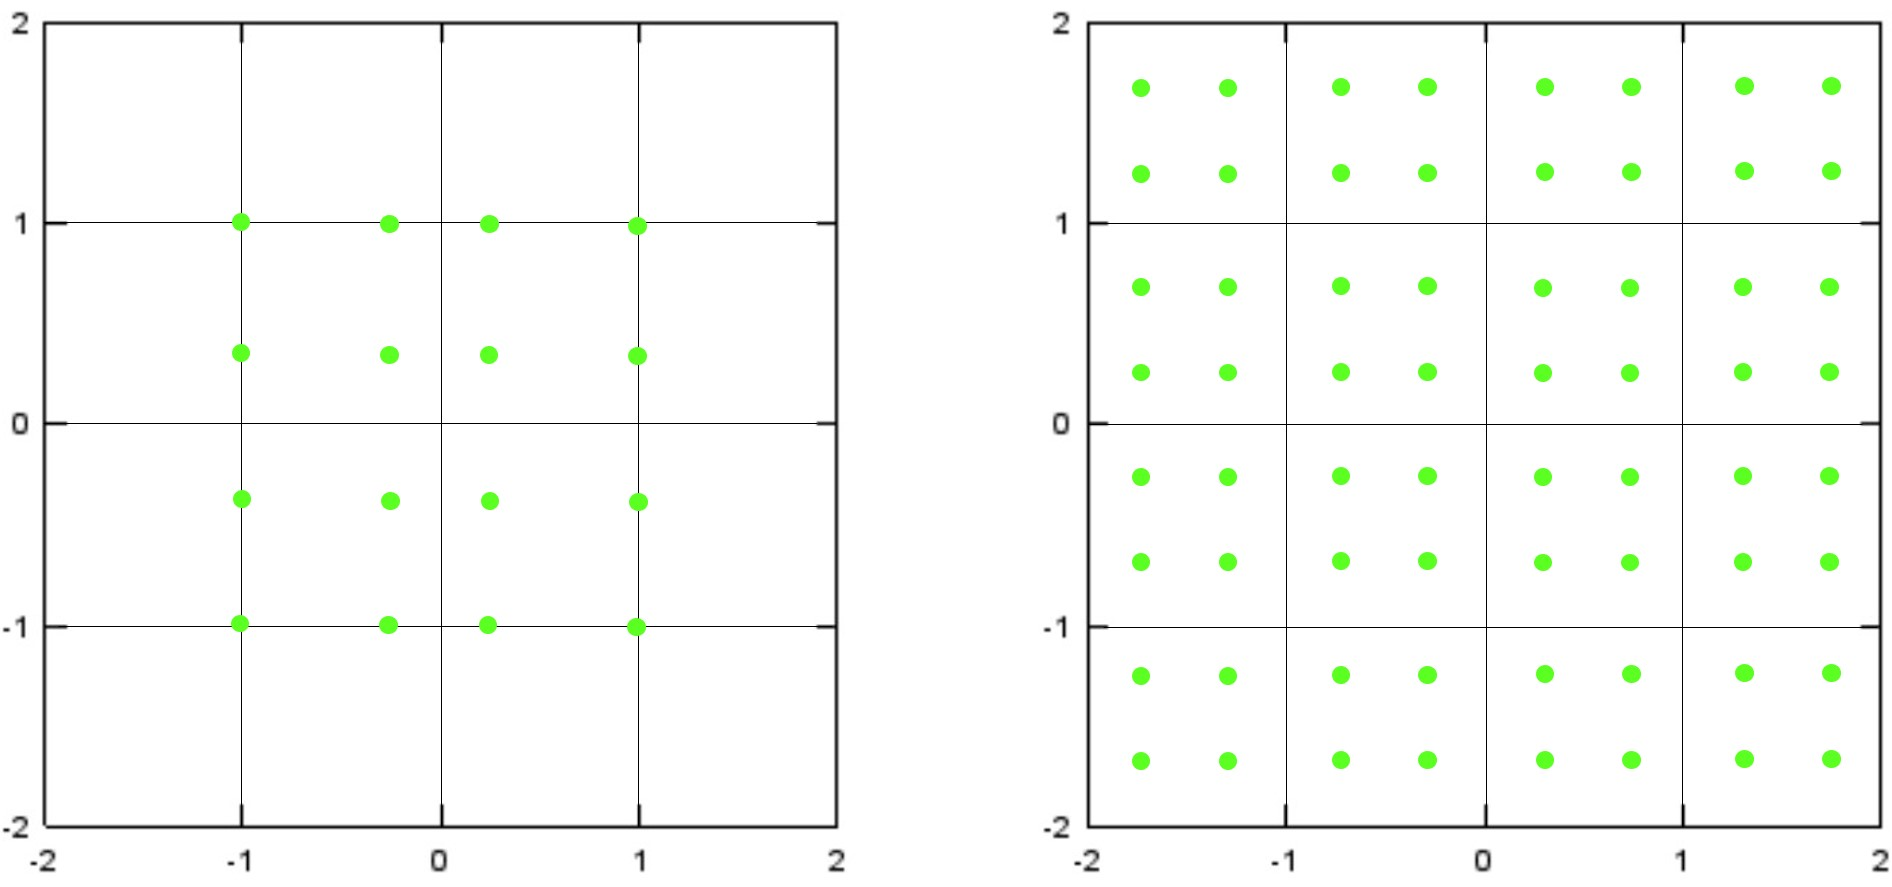
\includegraphics[width=0.9 \textwidth]{qam.jpg}
	\caption[Konstellationsdiagramm 16-\gls{acr:QAM} und 64-\gls{acr:QAM}]{Konstellationsdiagramme mit  16-\gls{acr:QAM} und 64-\gls{acr:QAM}} 
	\gls{online:Eigen}\gls{online:konst}
	\label{fig:qam}
\end{figure}



\subsection{Orthogonales-Frequenzmultiplexverfahren}
\label{subsec:ofdm}
Bevor im Verlauf dieses Kapitels das \gls{acr:OFDM} erläutert wird, muss vorher noch ein weiterer Begriff eingeführt werden. Hierbei handelt es sich um die Bandbreite. Die Bandbreite ist in der Signalverarbeitung eine Kenngröße, welche im Frequenzspektrum die Breite des Intervalls festlegt, in dem die bestimmenden Frequenzanteile eines zu übertragenden Signals liegen. Im vorausgehenden Abschnitt wurden Signale nur im komplexen Basisband betrachtet. Um jedoch Signale drahtlos zu übertragen, müssen diese in Bandpasslage transformiert werden in welcher sie durch obere und untere Grenzfrequenzen charakterisiert werden.\cite{hftech} Da es sich beim Basisband um den natürlichen Frequenzbereich eines Nutzsignals handelt muss der Bandpassbereich noch näher ausgeführt werden. Im Falle dieser Abschlussarbeit bei Audiosignalen also zwischen 0Hz und 20kHz, was als Bandbreite B bezeichnet wird. Reelle Basisbandsignale wie Audio, weisen jedoch sowohl positive als auch negative spektrale Anteile auf. Aufgrund dessen erstreckt sich die Bandbreite daher symmetrisch von $-B$ bis $+B$. Bei digitalen Modulationsarten hingegen werden meist im komplexen Basisband verarbeitet, welches sich symmetrisch von $-B/2$ bis $+B/2$ erstreckt. Vor der Modulation und nach der Demodulation liegt das Signal im Basisband. Nach der Modulation und vor der Demodulation jedoch, ist das Nutzsignal nicht mehr in der Basisbandlage, sondern auf einen Träger aufmoduliert. Es befindet sich dann im Trägerfrequenzbereich, beziehungsweise dem sogenannten Bandpassbereich.\gls{online:basis} 

Da Signale meist nicht endlich sind, sondern eine unendliche Ausbreitung im Frequenzspektrum besitzen, wird die Bandbreite durch eine Kenngröße markiert. Dabei markiert die 3-dB-Bandbreite die Grenzfrequenz, da das Signal dort weniger als die
Hälfte der maximalen Leistung beherbergt.\gls{online:bandbreite} Hierbei wird das Spektrum des zu sendenden Signals sowohl in positiver als auch in negativer Richtung an den Ort der Trägerfrequenz verschoben. Die benötigte Bandbreite eines Signals wird durch das Nyquist-Theorem definiert. Dabei steht $B$ für die Bandbreite und $f_{s}$ für die Symbolfrequenz des Signals.

\begin{equation}
	\label{equ:bandbreite}
	B = 2 \cdot f_{s}
\end{equation}

Die Bandbreite ist in der Kommunikationstechnik außerdem sehr begrenzt weshalb die Optimierung der Bandbreiteneffizienz eine große Rolle spielt. So werden hier möglichst schmalbandige Pulsformungen verwendet um diese Effizienz zu steigern.\cite{howwireless} Zudem muss die Bandbreite von  beispielsweise dem Netzbetreiber unter sehr vielen Teilnehmern so aufgeteilt werden, dass jeder möglichst störungsfrei nur das empfängt was er Empfangen soll. Um dies zu realisieren wurde der Mehrkanalzugriff entwickelt. Hierbei gibt es einige verschiedene Verfahren welche in Tabelle~\ref{tab:multiplex} näher erläutert werden und diesen Ansatz verfolgen. 

\begin{table}[htb]
	\begin{center}
		\begin{tabular}{p{0.33\textwidth}  p{0.6\textwidth}}
			\toprule
			\textbf{Multiplexverfahren} &  \textbf{Definition} \\ 
			\midrule
			Raummultiplexverfahren	& Um jeden Sender eine Zone eingerichtet, in der kein anderer Sender auf dergleichen Frequenz sendet. Damit können die benutzten Frequenzen (Kanäle) mehrfach vergeben werden, denn gegenseitige Störungen sind ausgeschlossen. Dieses Verfahren ist jedoch nicht für Mobilfunkanwendungen mit mehreren Teilnehmern im selben Bereich verwendbar.\\
			\midrule
			Zeitmultiplexverfahren	& Keine räumliche Trennung der genutzten Bandbreite, sondern  eine Trennung der vorhandene Bandbreite in Zeitschlitze. So wird jedem Teilnehmer ein gewisser Zeitraum zum Senden und Empfangen bereitgestellt. In diesem Zeitraum steht dem Teilnehmer die gesamte Bandbreite  des Kanals zur Verfügung, jedoch entstehen bei einer hohen Anzahl von Teilnehmern gezwungenermaßen längere Pausen. Bei einer Echtzeit-Audioübertagung, also einem Telefongespräch, muss der Sender in den Pausen die Daten in einem Buffer abspeichern und Paketweise versenden. Der Empfänger speichert die Daten in einem Buffer, um die Übertragungspausen zu überspielen und dann anhand der empfangenen Pakete in Echtzeit wiederzugeben.\\
			\midrule
			Frequenzmultiplexverfahren	& Ein nachrichtentechnisches Multiplexverfahren, bei dem gleichzeitig mehrere Signale auf mehrere Träger verteilt übertragen werden können. Die Träger sind vielen unterschiedlichen Frequenzen zugeordnet, weswegen auch der Begriff Frequenzmultiplex verwendet wird.\\	
			\bottomrule
\end{tabular}
\caption{Multiplexverfahren}\gls{online:ofdm}\cite{NT}
\label{tab:multiplex}
\end{center}
\end{table}

Allerdings wurde das in Tabelle~\ref{tab:multiplex} ausgeführte \gls{acr:FDM} noch weiterentwickelt und modifiziert. Beim normalen \gls{acr:FDM} können die Teilnehmer parallel Daten übertragen, dabei wird die Datenrate jedoch reduziert, da die zur Verfügung stehende Bandbreite kleiner wird und somit zwangsweise die Symbolfrequenz sinkt. Des Weiteren ist in Abbildung~\ref{fig:ofdm} zu erkennen, dass die Teilbänder nicht direkt nebeneinander positioniert sind. Dementsprechend entstehen Lücken im Spektrum, welche von keinem Teilnehmer belegt werden, wodurch die Bandbreite nicht effizient genutzt wird. Diese Lücken werden auch Sicherheitsband genannt und dienen der Vermeidung von Interkanal-Interferenzen. Diese entstehen, wenn zwei Kanäle zu nahe aneinander positioniert sind und sich deshalb gegenseitig stören. Der Nachteil ist jedoch, dass diese Sicherheitsbänder gleichzeitig auch die genutzte Bandbreite verringern und somit auch den Durchsatz an Daten. Zur Optimierung dieses Verfahrens wurde das Orthogonale-Frequenzmultiplexverfahren (\gls{acr:OFDM}) entwickelt.

\begin{figure}[h]
	\centering
	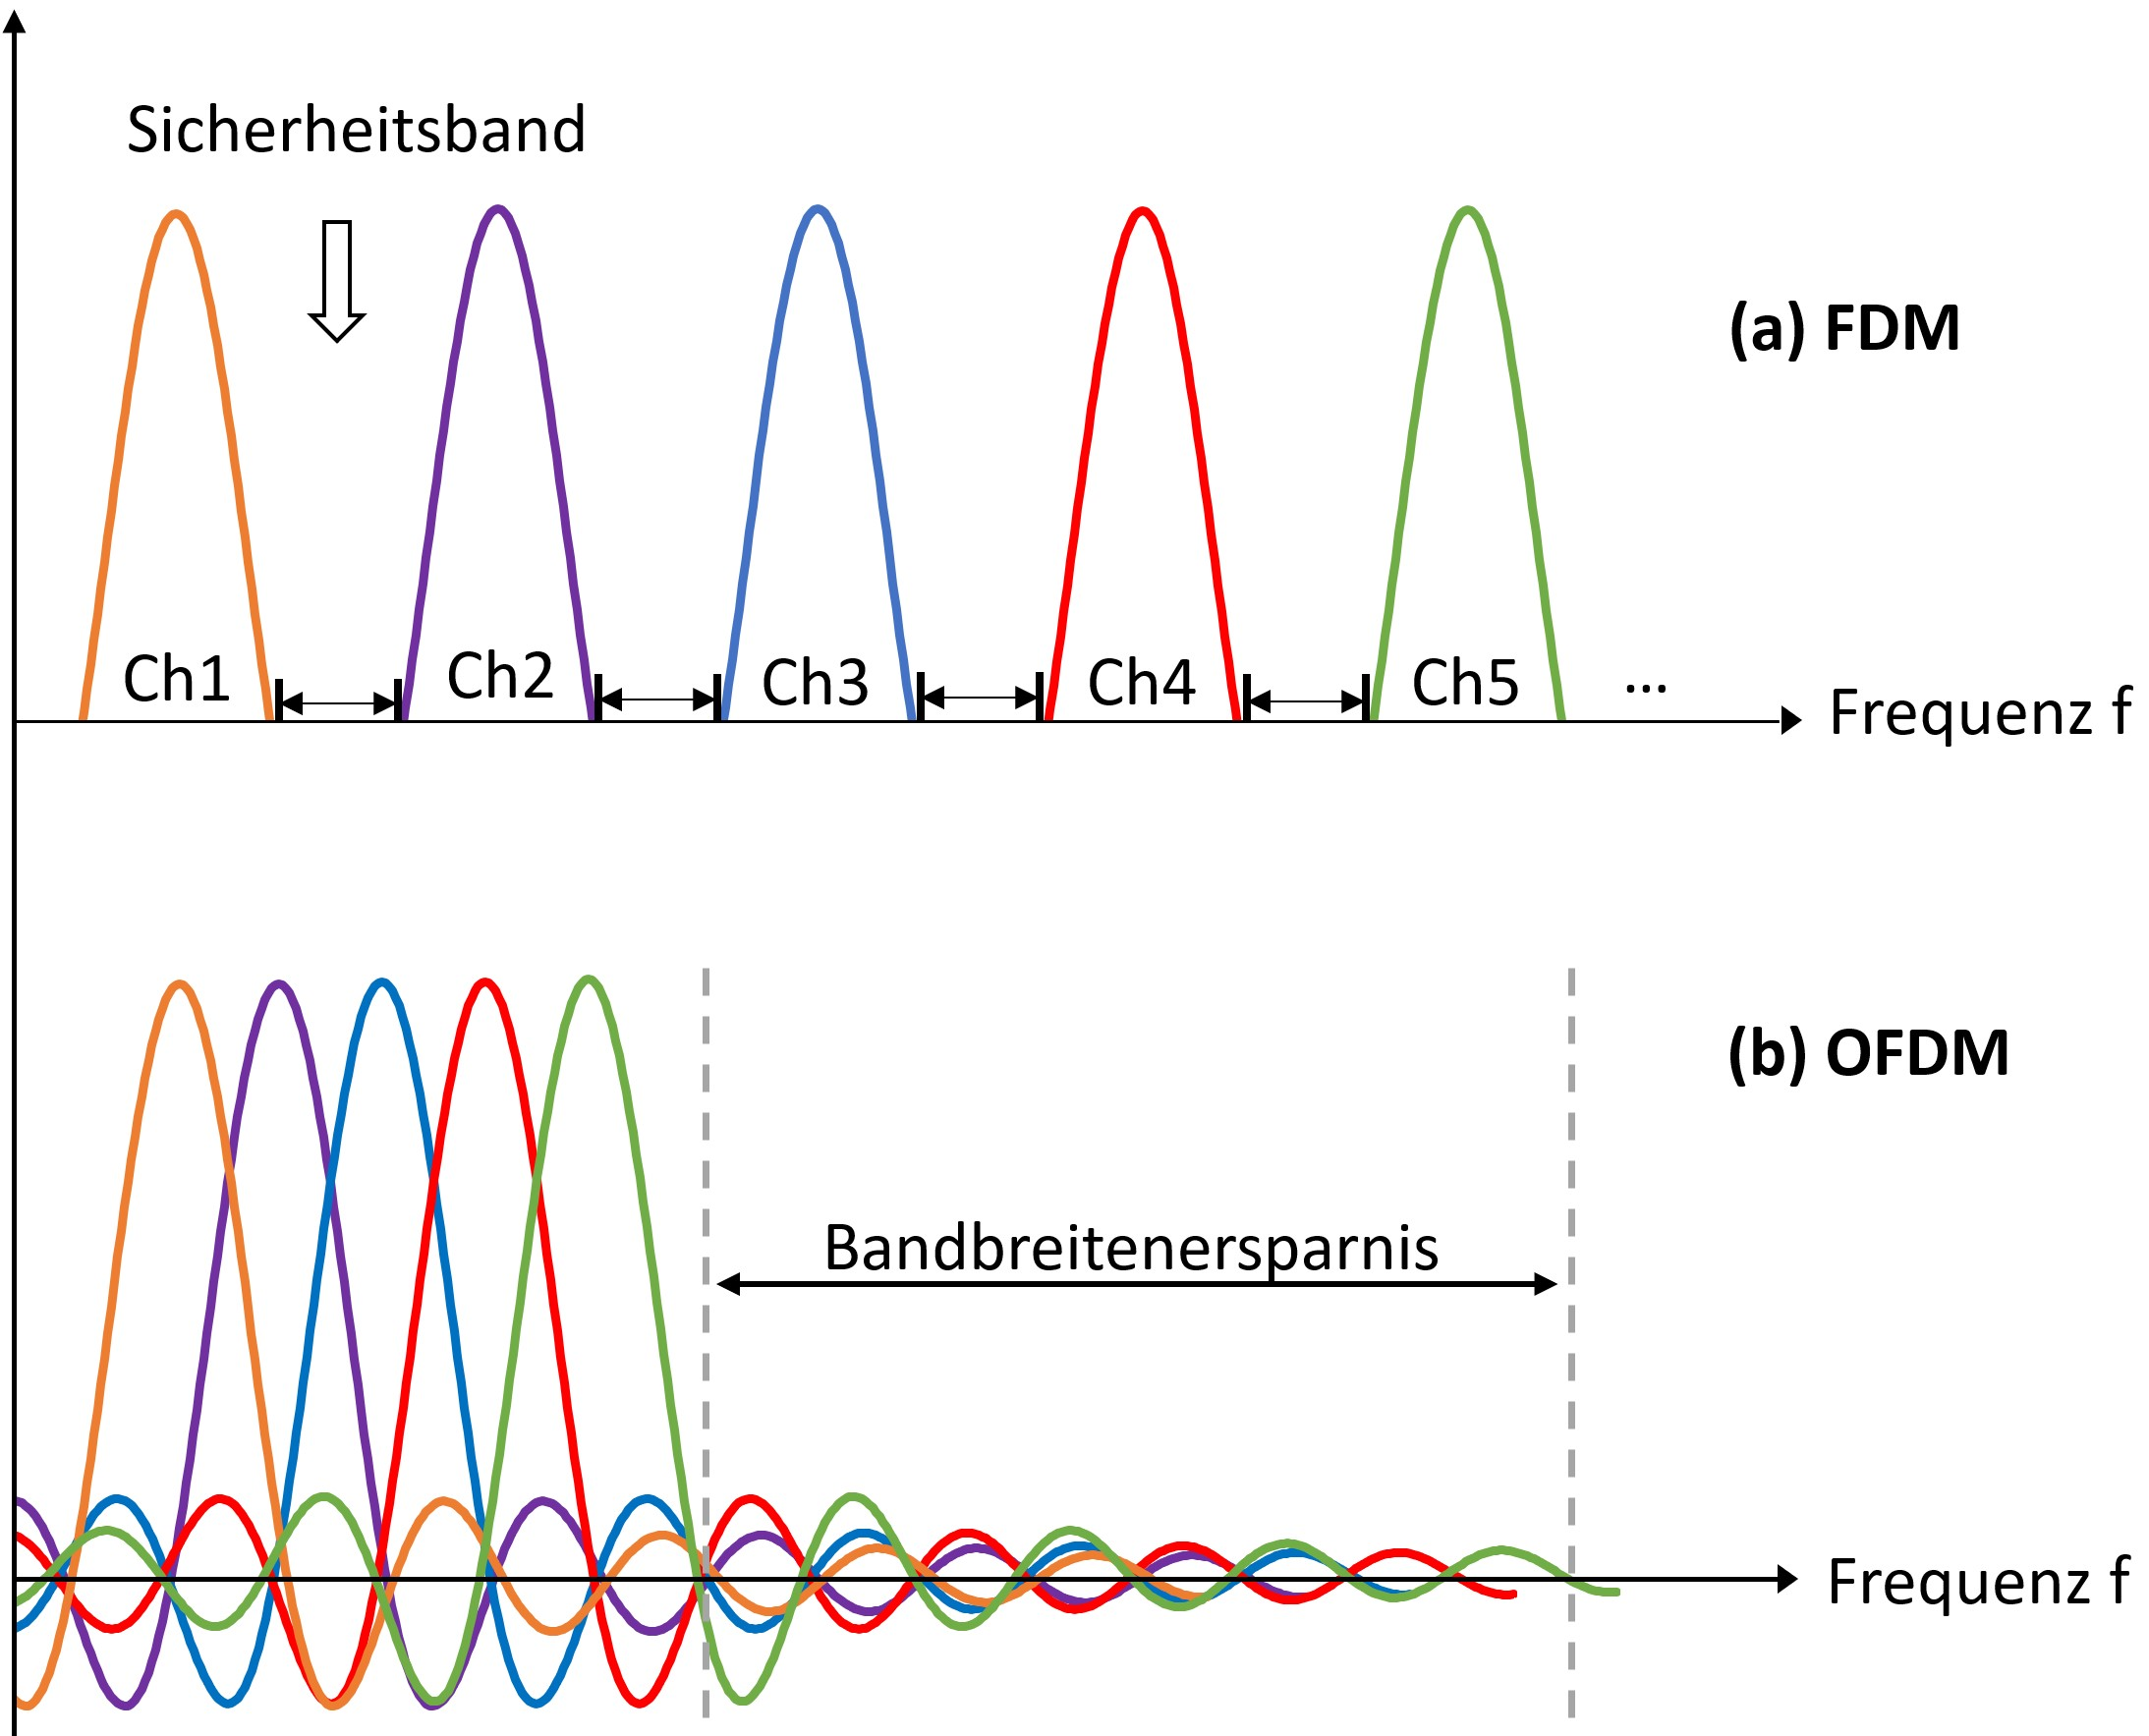
\includegraphics[width=0.75\textwidth]{ofdm.jpg}
	\caption[Spektrale Effizienz des Orthogonalen-Frequenzmultiplexverfahren]{Spektrale Effizienz des Orthogonalen-Frequenzmultiplexverfahren} 
	\gls{online:Eigen}
	\label{fig:ofdm}
\end{figure}

Bei diesem Verfahren werden die Tägerwellen so angeordnet, dass ein Maximum eines Trägers bei seinen Nachbarträgern jedes Mal auf einem Nulldurchgang liegt. Aus dieser orthogonalen Trägerbeziehung ergibt sich der Name dieses Verfahrens. Zudem wird es nicht nur verwendet, um die Bandbreite für diverse Teilnehmer aufzuspalten, sondern unterteilt entsprechend die einzelnen Teilbänder in viele kleinere Bänder, welche von mehreren Teilnehmern genutzt werden können. Datenpakete werden also nicht Seriell sondern Parallel versendet.\gls{online:ofdm} Kommt es innerhalb des \gls{acr:OFDM}-Signalspektrums zu einer schmalbandigen Störung, können die von der Störung betroffenen Träger von der Datenübertragung ausgenommen werden, wodurch die Datenrate nur minimal sinkt. Bei einer \gls{acr:QAM} welche breitbandig mit nur einem Träger übertragen wird, kann dahingegen eine schmalbandige Störung im Übertragungskanal die ganze Datenübertragung gefährden.\cite{butlerWirelessNetworkingDeveloping2013} Bei der \gls{acr:OFDM} wird demnach durch das realisieren schmalerer Bänder die Fehlerwahrscheinlichkeit gesenkt. So werden beim \gls{acr:OFDM}-Verfahren jeweils nur einzelne Träger durch Interferenzen aufgrund von Mehrwegeausbreitung betroffen.\cite{NT}

\subsection{Digital Radio Mondiale}
\label{subsec:drm}
Seit Anbeginn des Rundfunks verwenden fast alle Mittelwellen- und Langwellensender die \gls{acr:AM} zur Übertragung von Audiosignalen. Das Problem hierbei ist, dass das Modulationsschema und die geringe Kanalbandbreite von 10 kHz die Audioqualität immens einschränken. Deshalb werden in diesen Bändern üblicherweise Sprachsignale übertragen. Ende 2003 veröffentlichte das \gls{acr:ETSI} die Spezifikation für den digitalen Rundfunk bei 30 MHz unter Verwendung des \gls{acr:OFDM} Mehrträgerverfahrens. Das System wurde \gls{acr:DRM} genannt. 

\begin{figure}[H]
	\centering
	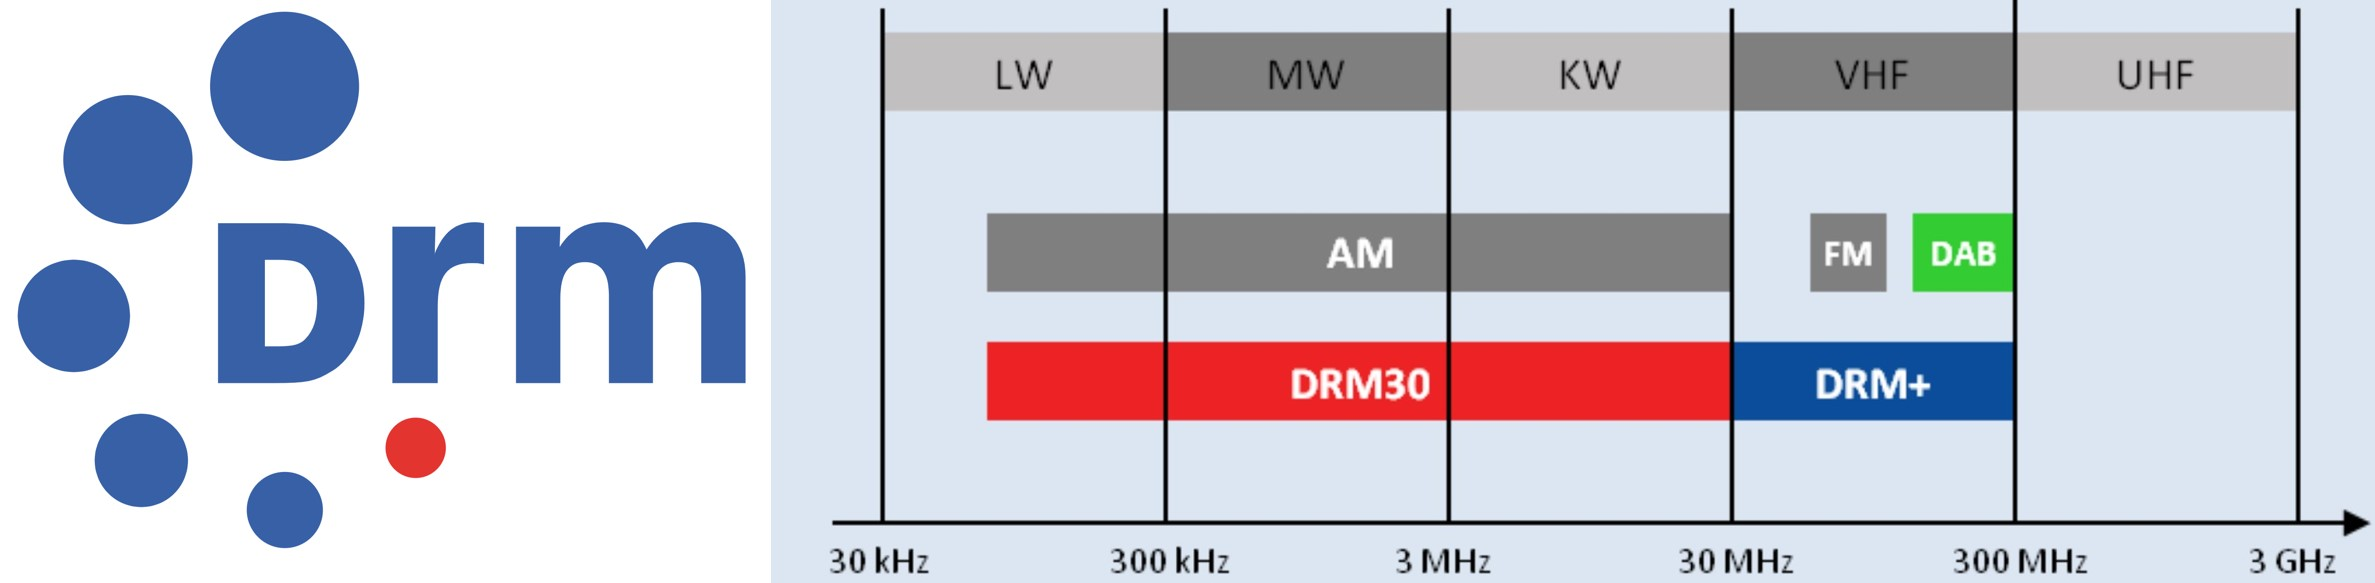
\includegraphics[width=1 \textwidth]{drmfreq.jpg}
	\caption[\gls{acr:DRM} - Frequenzbereich]{\gls{acr:DRM} - Frequenzbereich} 
	\gls{online:drmpic}
	\label{fig:drmfreq}
\end{figure}

Bezogen auf die Kanalbandbreite von 10 kHz ist die Datenrate der gestreamten Medien auf etwa 35 kBit/s bei einem Kanal und 72 kBit/s bei Verwendung von zwei Kanälen beschränkt. Obwohl die Bitrate nicht sehr hoch ist, übertrifft die Audioqualität der Streams die Qualität von \gls{acr:FM}-Mono-Übertragungen bei weitem. Der erweiterte Audio-Codierungsstandard \gls{acr:AAC} in Kombination mit \gls{acr:SBR} (eine Verlustbehaftete Audiodatenkompression) und parametrischem Stereo bietet hohe Audioqualität bei sehr niedrigen Bitraten (z. B. 22 kBit/s). Und ist somit ein qualitativ hochwertiger digitaler Ersatz für den derzeitigen analogen Hörfunk in den \gls{acr:AM}- und \gls{acr:FM}/\gls{acr:VHF}-Bändern. Eine Übersicht über die Frequenzbänder, in welchen \gls{acr:DRM} arbeitet, wird in Abbildung ~\ref{fig:drmfreq} Dargestellt. Zudem ist die \gls{acr:DRM}-Übertragungskette durch die drei Kanäle \gls{acr:MSC}, \gls{acr:SDC} und \gls{acr:FAC} gekennzeichnet. Diese werden in Abildung~\ref{fig:drm} illustriert.\gls{online:drm}



\begin{figure}[H]
	\centering
	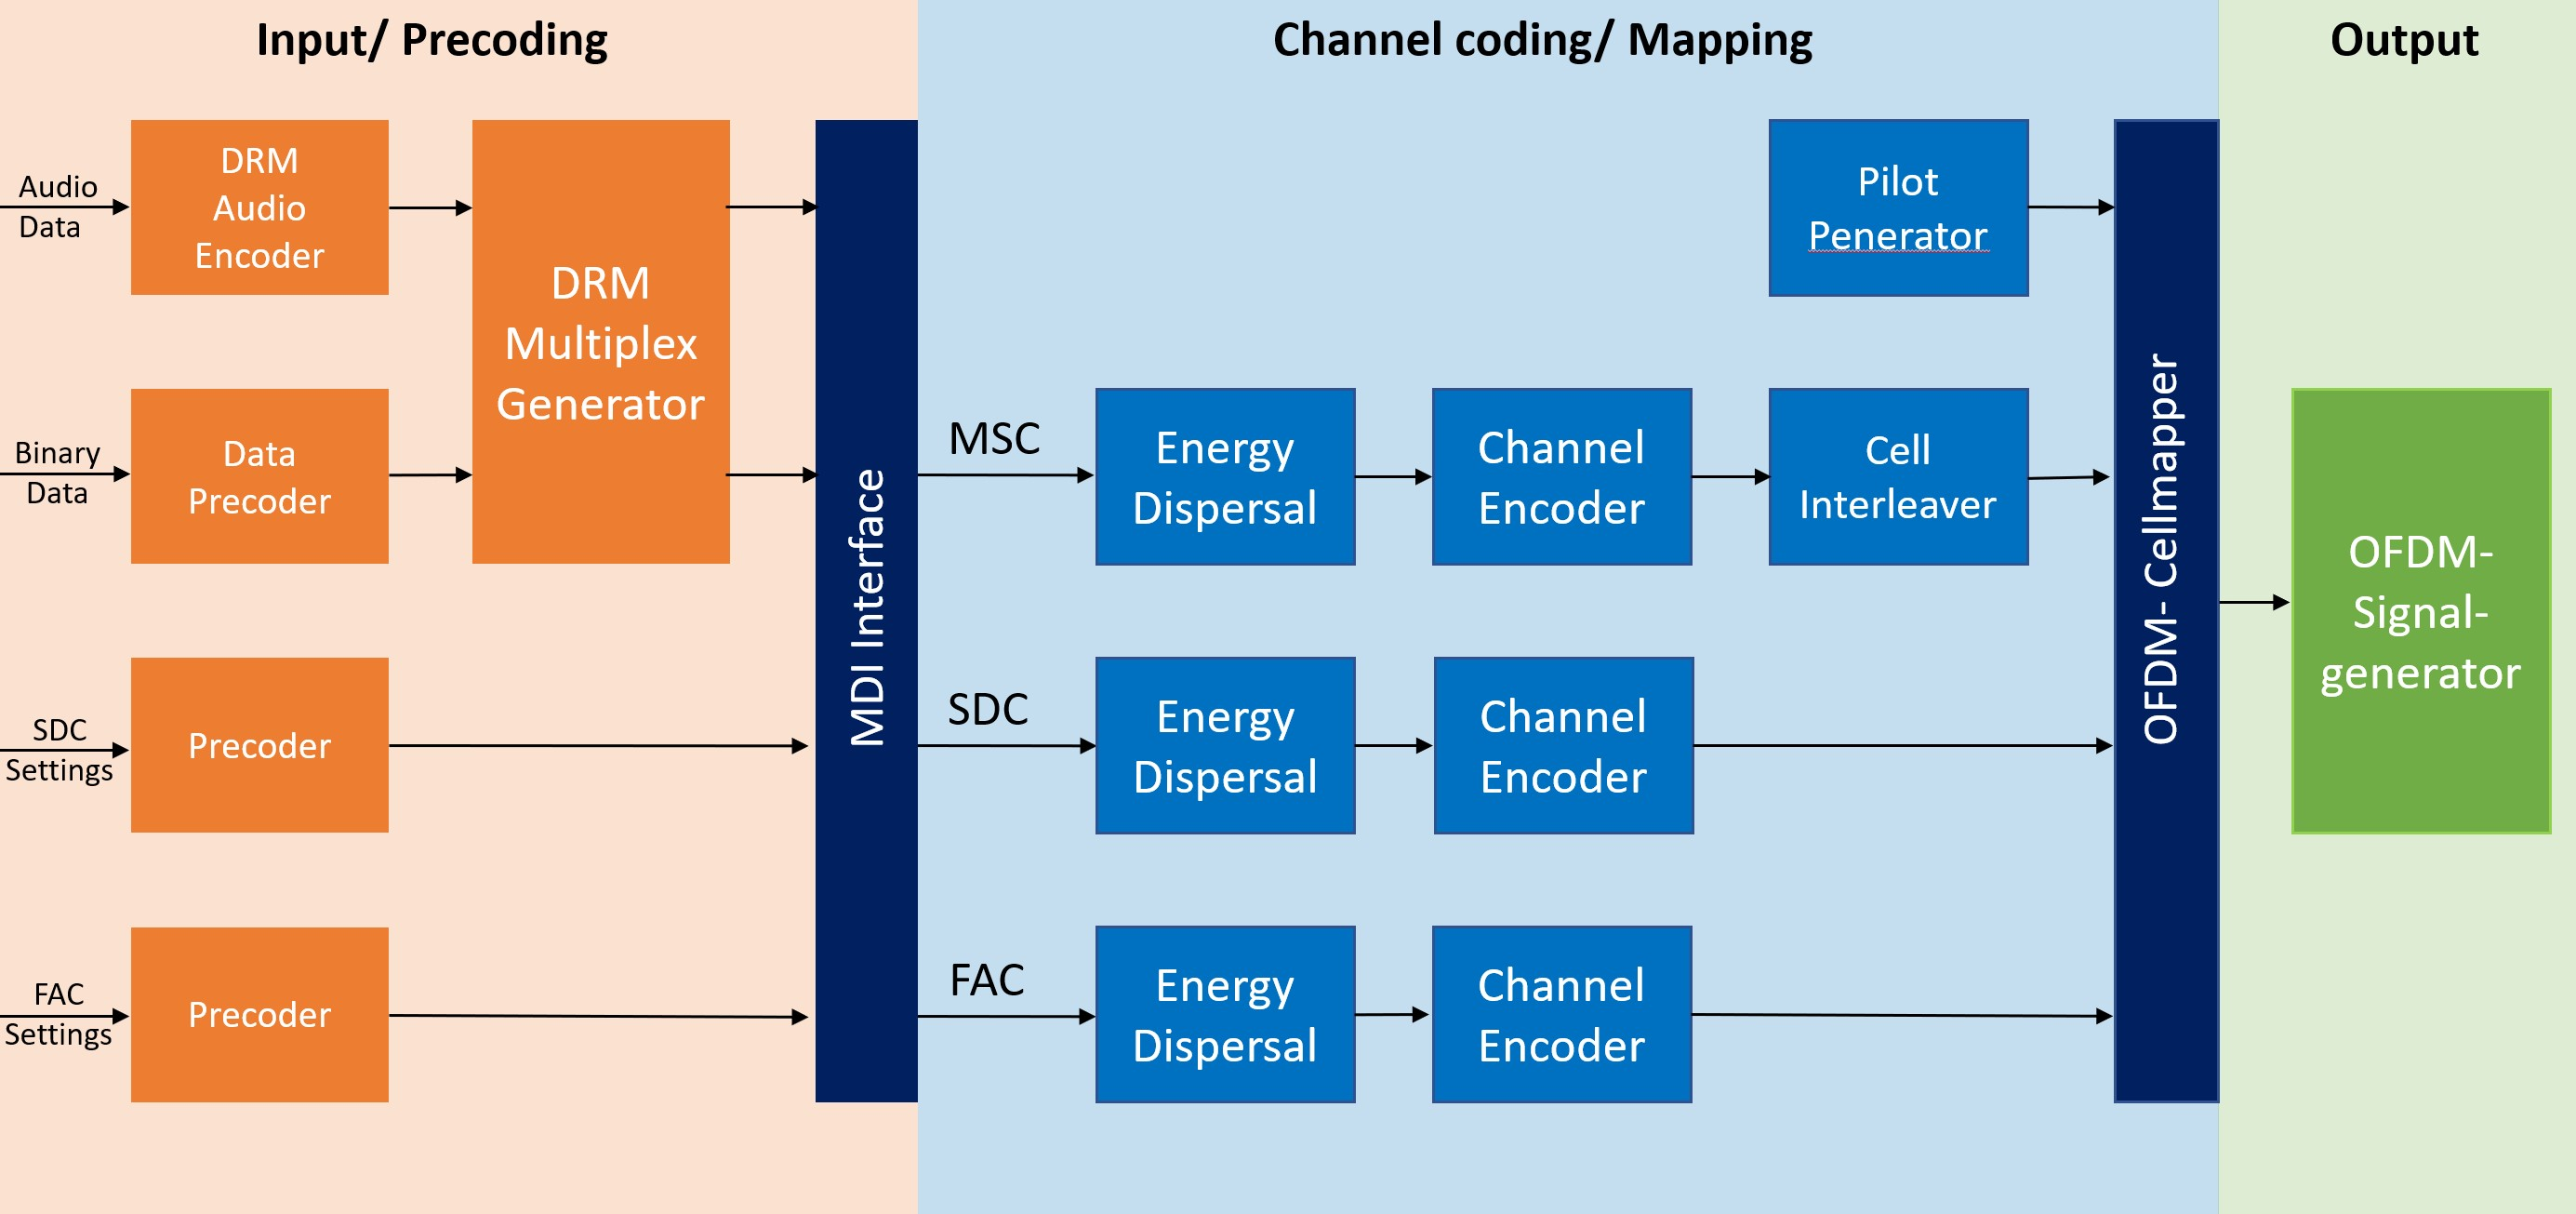
\includegraphics[width=0.85 \textwidth]{drm.jpg}
	\caption[DRM - Struktur]{DRM - Struktur} 
	\gls{online:Eigen}
	\label{fig:drm}
\end{figure}
Hierbei wird der \gls{acr:FAC} vom Empfänger verwendet, um Informationen über die \gls{acr:OFDM}-Signaleigenschaften und die \gls{acr:SDC}/\gls{acr:MSC}-Konfiguration zu erhalten. Für die korrekte Synchronisation und \gls{acr:SDC}/\gls{acr:MSC}-Interpretation liest ein Empfänger die Belegung des Spektrums, den Trägerabstand und die \gls{acr:QAM}-Auflösungsinformationen im \gls{acr:FAC}-Datenblock. Die feste Coderate von 0,6 und die Verwendung von \gls{acr:QAM}-Codierung machen den \gls{acr:FAC} sehr robust gegenüber Fehlern. \gls{online:drm}\gls{online:drmpic} Die Coderate steht hierbei für das Verhältnis der Informationssymbole zur Länge der übertragenen Wörter.

Der \gls{acr:SDC} enthält die für die \gls{acr:MSC}-Dekodierung benötigten Informationen, wie die Multiplex-Frame-Struktur und weitere Zusatzinformationen. Diese werden in einer sequentiellen Liste von Datenentitäten übertragen. Jeder Datenentitätstyp hat eine eindeutige Nummer, welche seine Datenstruktur definiert. Der Channel Encoder verwendet ein Standard-Mapping mit einer Modulation von 4-\gls{acr:PSK} oder 16-\gls{acr:QAM} und einer Gesamtcoderate von 0,5. Ebenso wie der \gls{acr:FAC} ist auch der \gls{acr:SDC} mit  \gls{acr:EEP}-kodiert und hat keinen hoch geschützten Bestandteil. Normalerweise wird der höher geschützte Teil mit einer höheren Coderate kodiert, was zu mehr Redundanz führt und somit die Wahrscheinlichkeit von Bitfehlern in schlechten Übertragungsszenarien verringert.\gls{online:drm}\gls{online:drmpic} 

Der \gls{acr:MSC} enthält die eigentlichen Audio- und Datenbits. Dieser kodiert den vom Multiplexer erzeugten Multiplexrahmen und verwendet, je nach Wahl des Users, entweder eine 16- oder 64-\gls{acr:QAM} mit verschiedenen Mapping-Schemata. Es besteht die Wahl zwischen Standard-Mapping, symetrisch-hierarchischem oder gemischt-hierarchischem Mapping, wobei nur das Standard-Mapping 16 \gls{acr:QAM} zulässt. Bei hierarchischer Modulation wird jedes Bit eines hierarchischen Multiplexrahmens auf einen komplexen Zellenquadranten abgebildet, was bei zu hoher Fehlerrate eine 4-\gls{acr:QAM}-Dekodierung der \gls{acr:MSC}-Zellen ermöglicht. Um das \gls{acr:MSC} noch fehlerresistenter zu machen, ist es möglich, \gls{acr:UEP} zu verwenden und den Multiplex-Rahmen in einen höher oder niedriger geschützten Datenteil aufzuteilen. Ein sogenanntes Cell-Interleaving von entweder 2s (lang) oder 400ms (kurz) schützt die \gls{acr:MSC}-Daten zusätzlich vor Fehlerbursts. \gls{online:drm}\gls{online:drmpic}  Burstfehler (auch Bündelfehler genannt) beschreiben blockweise Störungen eines Signals. Durch diese gestörten Blöcke, könnte es passieren das eine ganze Folge von Übertragenen Bits nicht mehr die gewünschte Information enthalten.\gls{online:burst} Abbildung~\ref{fig:burst} zeigt eine solche gestörte Bitfolge.
 \begin{figure}[H]
 	\centering
 	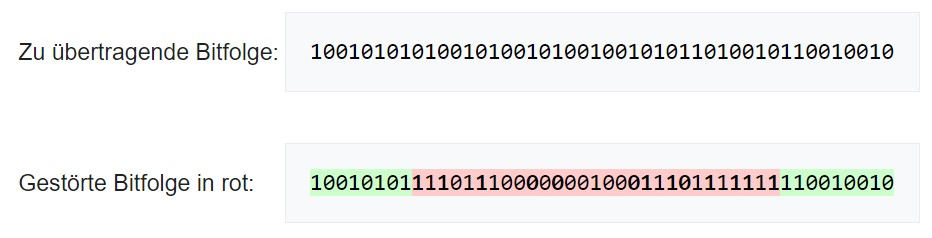
\includegraphics[width=0.7 \textwidth]{burst.jpg}
 	\caption[Burstfehler Beispiel]{Burstfehler Beispiel} 
 	\gls{online:burst}
 	\label{fig:burst}
 \end{figure}
Das \gls{acr:MDI} ermöglicht eine räumlich entfernte Verbindung zwischen dem \gls{acr:DRM}-Inhaltsserver und dem Basisbandmodulator (\gls{acr:MDI}-Empfänger) über Ethernet. Daher kann das analoge Basisbandsignal sehr nah am Sender erzeugt werden und es besteht keine Notwendigkeit für \gls{acr:HF}-Verbindungen über große Entfernungen, die dem Ausgangssignal viel Rauschen hinzufügen könnten.\gls{online:drm}\gls{online:drmpic} Um eine solche Struktur aufzubauen und \gls{acr:DRM} zu übertragen, wurde ein Programm namens Dream \gls{acr:DRM} verwendet. Dieses wird im weiteren Verlauf dieser Abschlussarbeit noch näher erläutert. 
\newpage
\section{Hardwarekomponenten}
\label{subsec:elbau}
Im letzten Kapitel wurden grundlegende Bestandteile einer digitalen Signalmodulation erörtert und das \gls{acr:DRM} eingeführt. Nun sollen relevante Bauteile eines \gls{acr:VLC}-Senders dargestellt und näher ausgeführt werden. Hierbei handelt es sich nun um jene Komponenten, welche als Sender und Kanal in Abbildung~\ref{fig:komsystem} charakterisiert wurden. Diese Hardwarekomponenten sind essenziell, um sowohl die analoge Signalverarbeitung, als auch die Datenübertragung mittels eines optischen Kanals zu ermöglichen. Es werden im Folgenden demnach verschiedene Bauteile und deren Bedeutung im Kontext zu dieser Abschlussarbeit verdeutlicht.

\subsection{Leuchtdiode}
\label{sub:led}

Eine \gls{acr:LED} ist ein Licht-emittierendes Halbleiter-Bauelement mit einem pn-Übergang. Ihre elektrischen Eigenschaften stimmen mit der einer Standard Diode überein, wodurch sie in nur eine Richtung leitend ist und in die entgegengesetzte Stromrichtung sperrt. Wenn durch einen eingekoppelten elektrischen Strom die \gls{acr:LED} in Durchlassrichtung betrieben wird, findet eine Lichtemission statt.\cite{slabke} 

\begin{figure}[H]
	\centering
	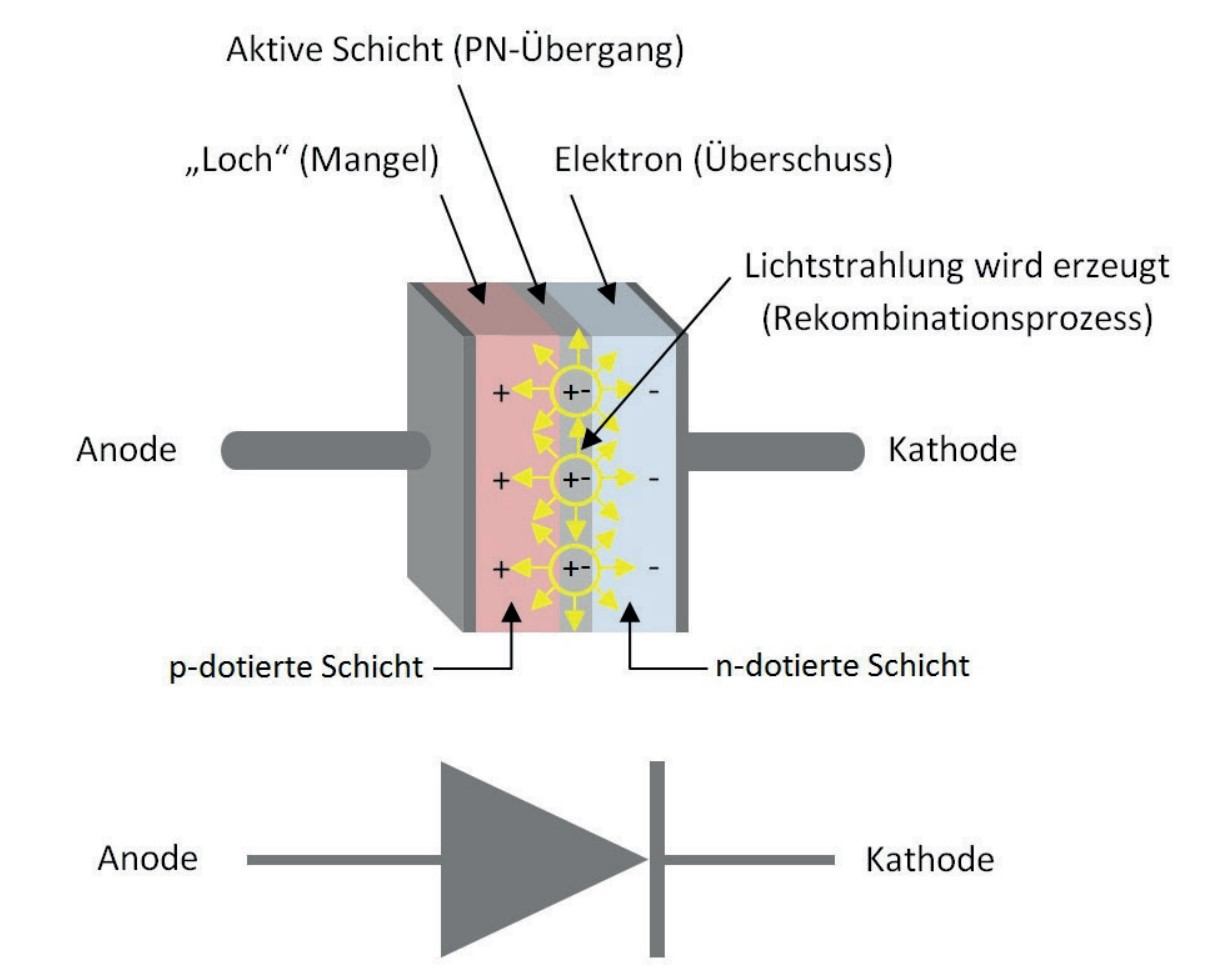
\includegraphics[width=0.65 \textwidth]{LED.jpg}
	\caption[Strahlungserzeugung in der LED am pn-Übergang]{Strahlungserzeugung in der LED am pn-Übergang} \cite{slabke}
	\label{fig:LED}
\end{figure}

Der Grundsatz der Lichterzeugung in einer \gls{acr:LED} beruht auf einem Halbleiterkristall, der durch das Einbringen von Fremdatomen so dotiert ist, dass in der Diode zwei Gebiete entstehen. In einem Gebiet entsteht ein Elektronenüberschuss und in dem anderen Gebiet entstehen Löcher. Durch das Injizieren von Elektronen aus der positiv dotierten Seite in die Sperrschicht rekombinieren sich Löcher und Elektronen, wodurch Energie in Form von Licht abgegeben wird.\cite{slabke} Die Farbe hängt dabei vom Halbleitermaterial und der genauen Dotierung ab. Zudem ist dieser Rekombinationsprozess stark temperaturabhängig.\cite{heringElektrotechnikUndElektronik2018}  Wie dieser thermische Faktor jedoch gedämpft wird, wird in einem noch folgenden Kapitel näher erläutert.

\begin{figure}[H]
	\centering
	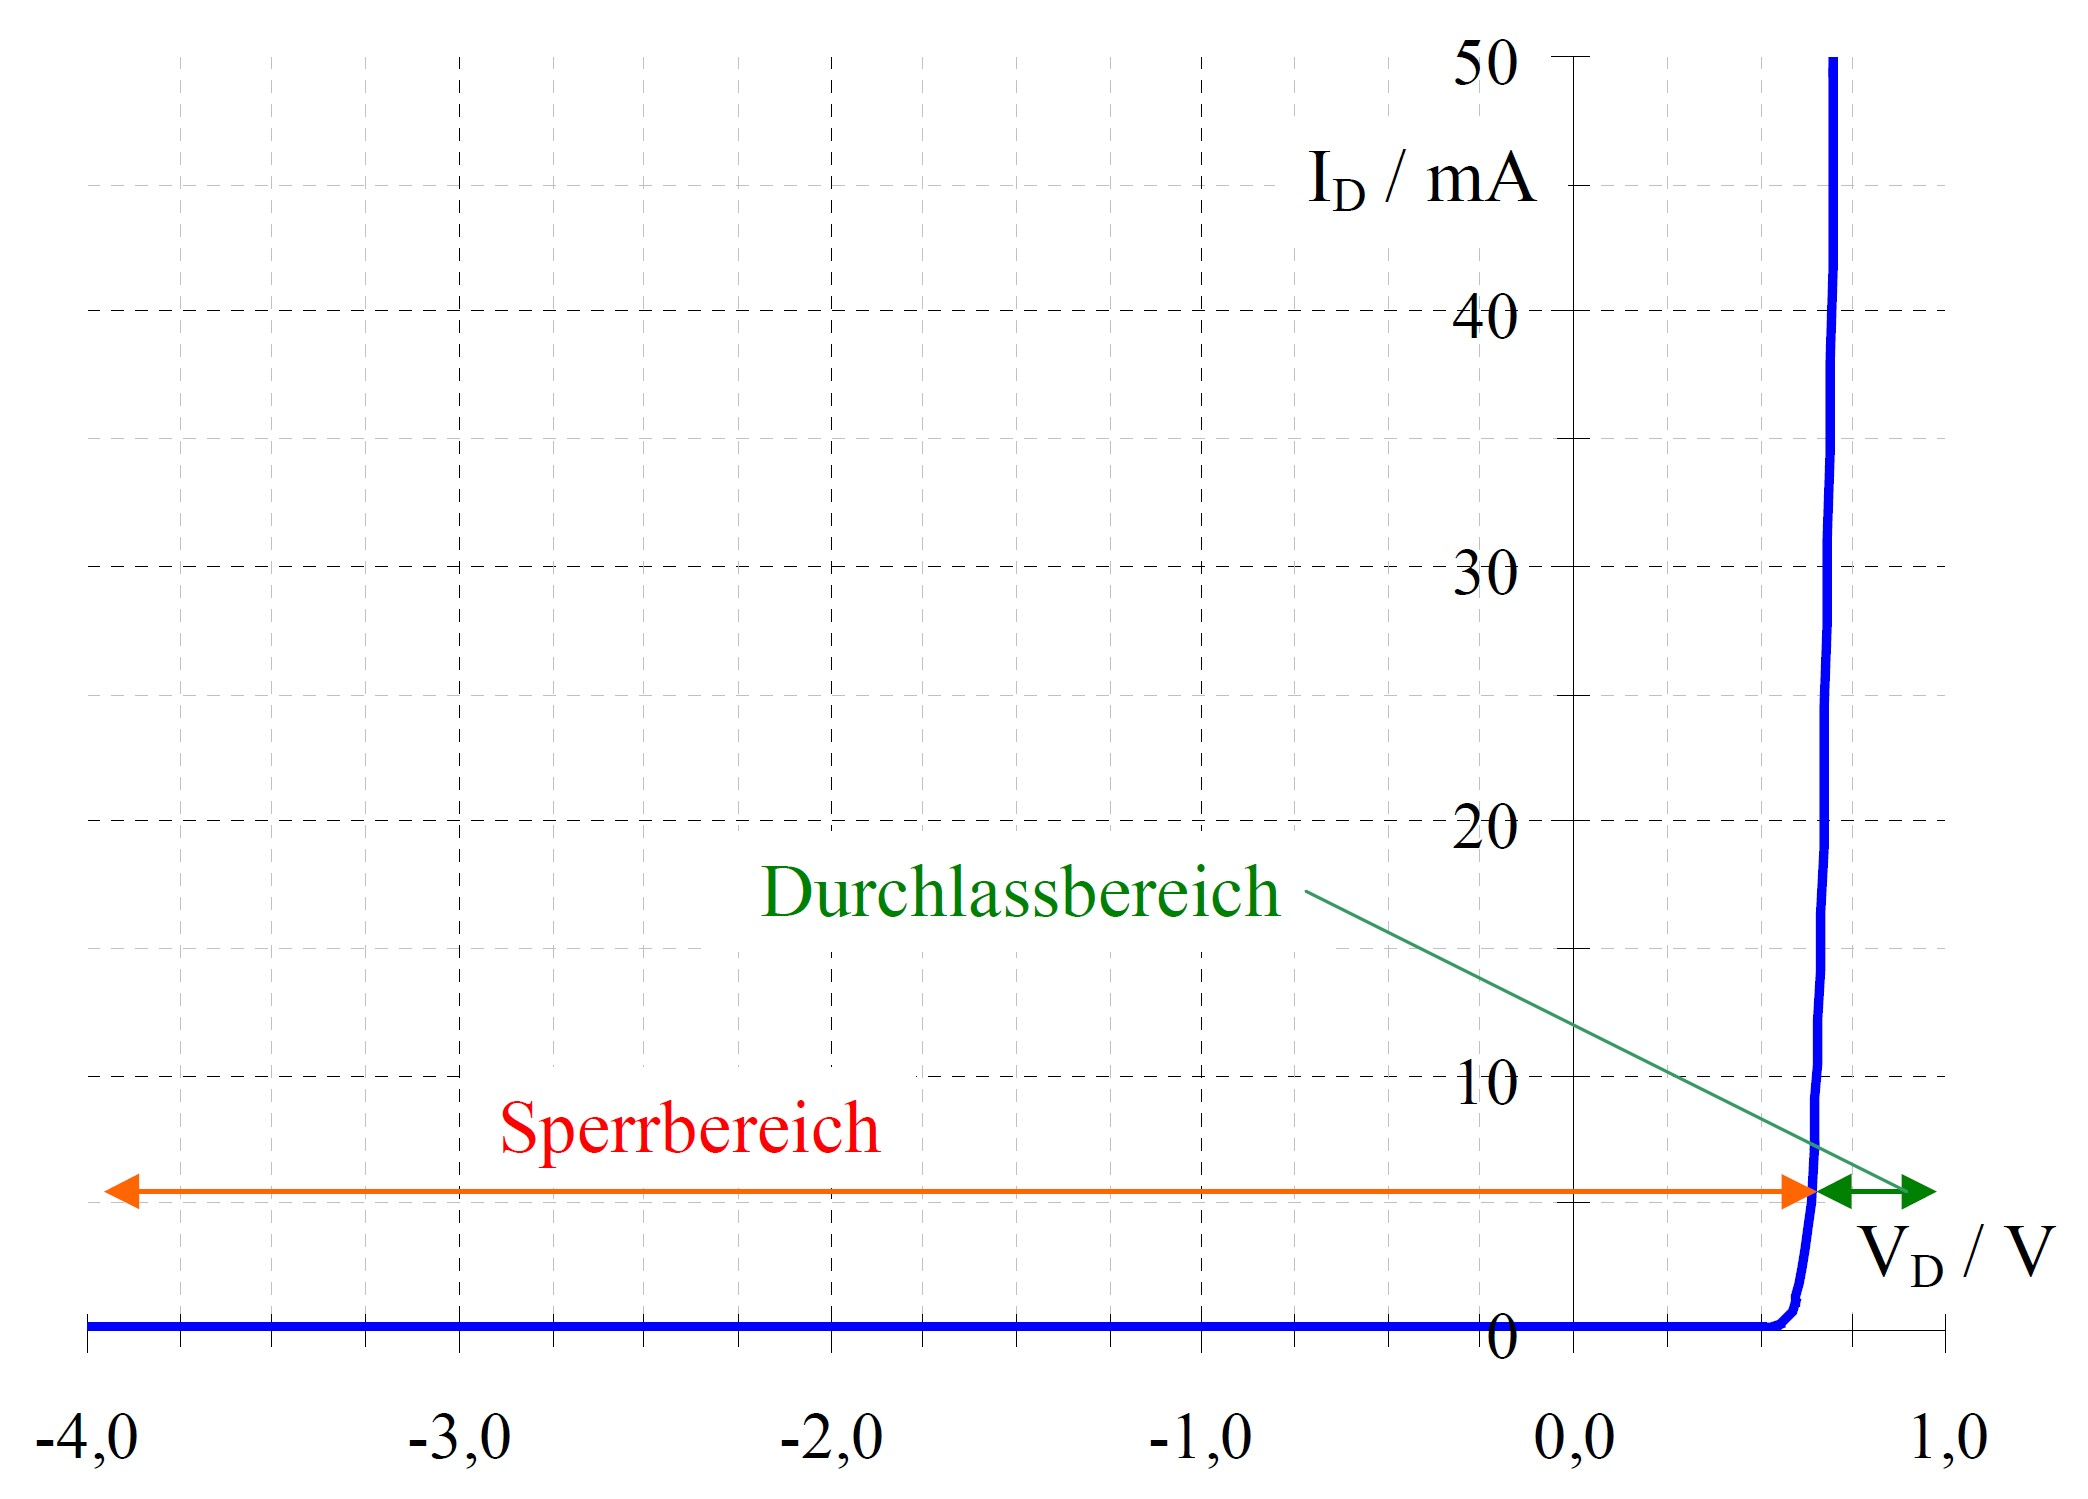
\includegraphics[width=0.55 \textwidth]{Kennlinie.jpg}
	\caption[Diodenkennlinie]{Diodenkennlinie} 
	\gls{online:elektronik}
	\label{fig:Kennlinie}
\end{figure}

In der Abbildung ~\ref{fig:Kennlinie} ist die Strom-/Spannungskennlinie einer Diode in Durchlassrichtung
dargestellt. Die Kennlinie einer LED hat den selben Verlauf, jedoch liegt die Durchlassspannung je nach gewählter Farbe nicht bei ca. 0.7V sondern im Bereich von 1,6V (rote \gls{acr:LED}) bis zu 4V (blaue \gls{acr:LED}) .\gls{online:elektronik} 

\begin{figure}[H]
	\centering
	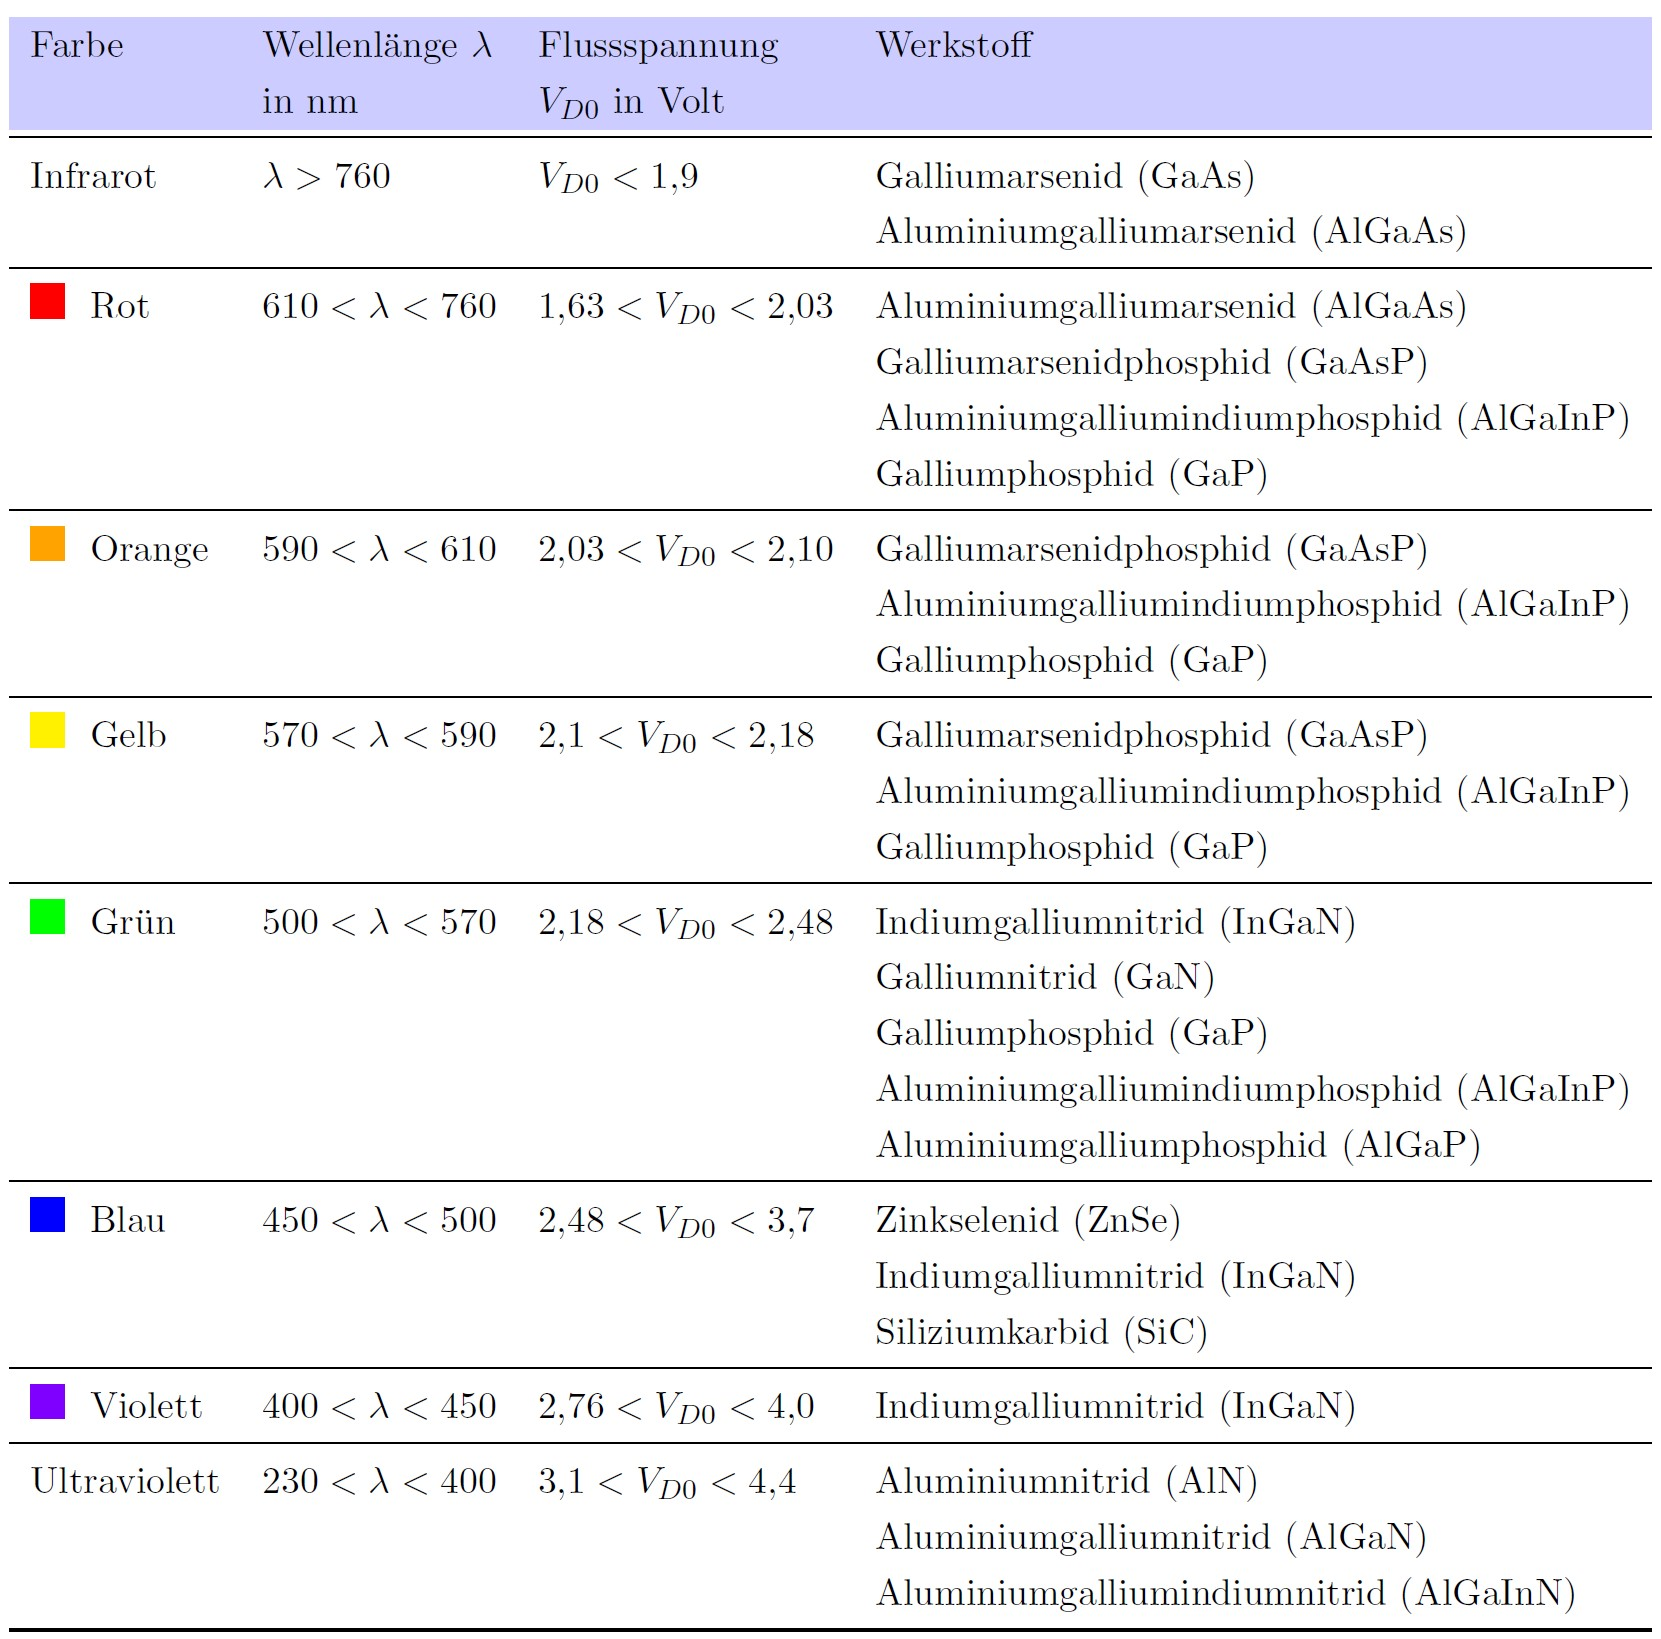
\includegraphics[width=0.75 \textwidth]{Flussspannung.jpg}
	\caption[Flussspannungen von \gls{acr:LED}s verschiedener Farben]{Flussspannungen von \gls{acr:LED}s verschiedener Farben} 
	\gls{online:elektronik}
	\label{fig:Flussspannung}
\end{figure}

Wie in Abbildung ~\ref{fig:Kennlinie} illustriert ist, ändert sich die Spannung in ihrem Verlauf ab einem gewissen Punkt nur noch minimal. Das bedeutet, dass sich ab einer gewissen angelegten Spannung lediglich der Strom noch weiter erhöhen kann. Da die Leuchtintensität der \gls{acr:LED} von dieser Höhe des Stromdurchflusses abhängt, führt dies zu dem Schluss, den durchfließenden Strom statt der angelegten Spannung zu regulieren. Wird nun der durch die \gls{acr:LED} fließende Strom mit der Ausgangsleistung ins Verhältnis gesetzt, ergibt sich ein Zusammenhang wie ihn Abbildung ~\ref{fig:Helligkeit} zeigt. 

\begin{figure}[H]
	\centering
	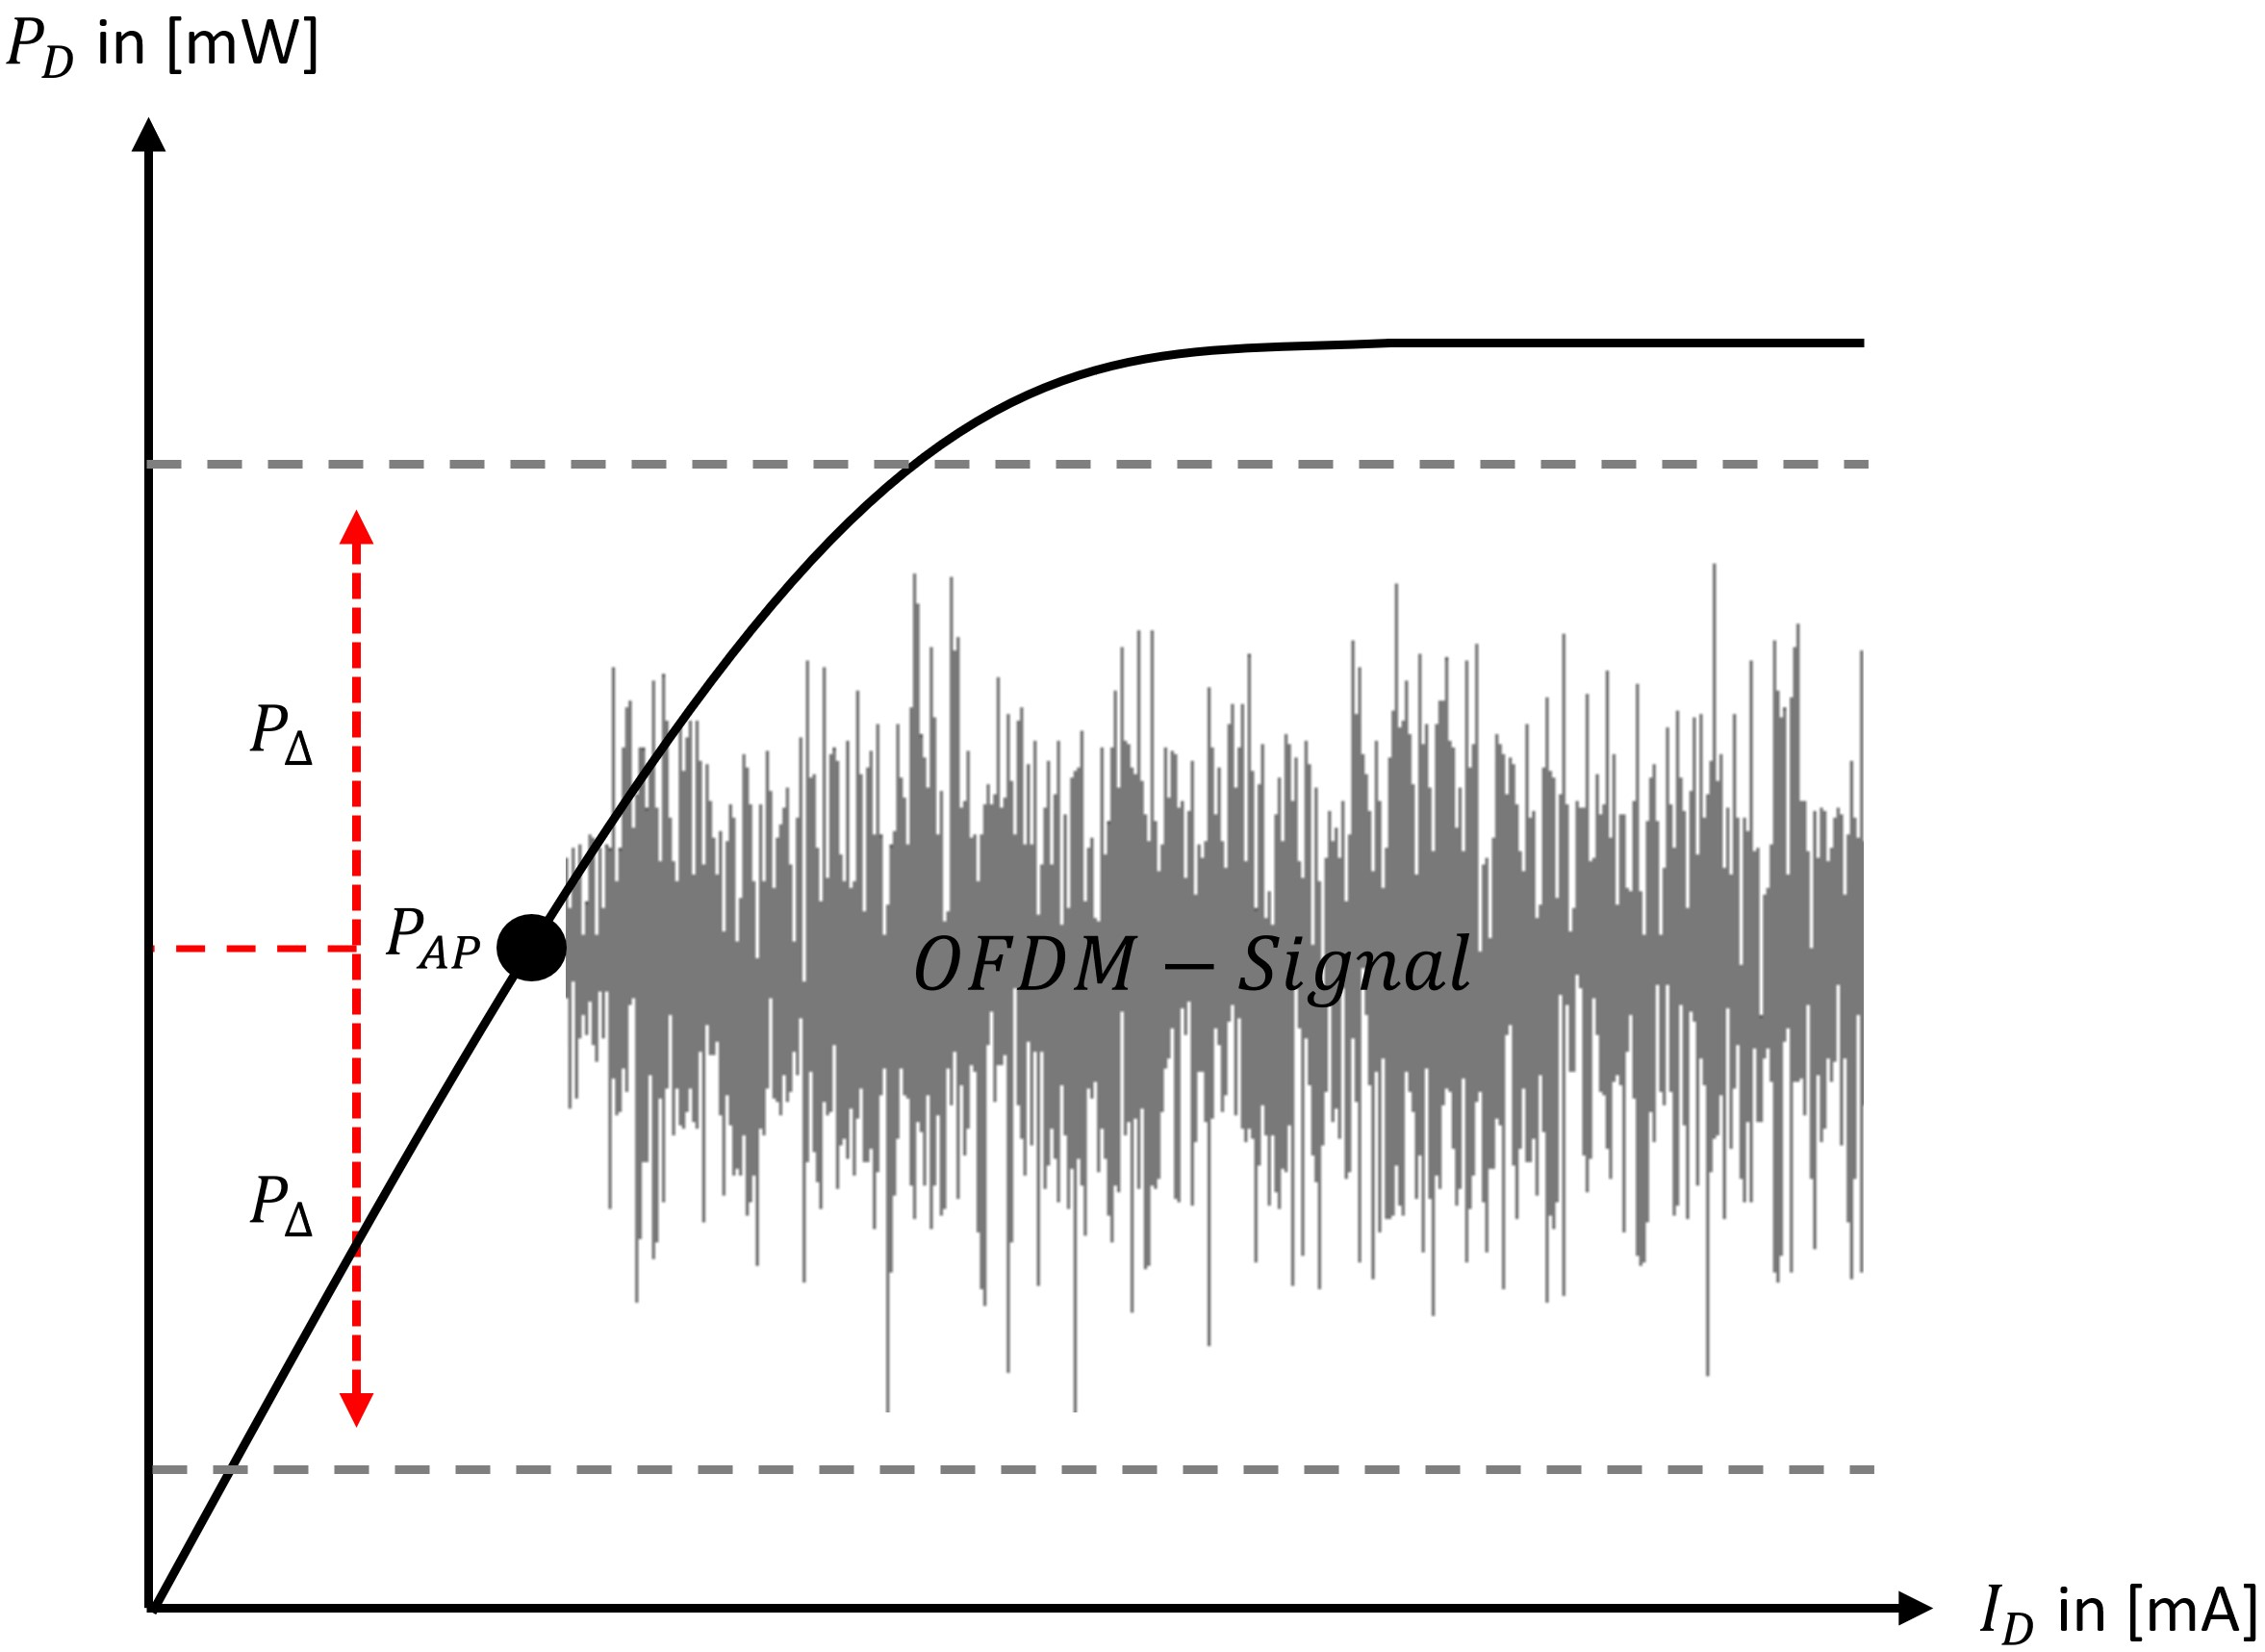
\includegraphics[width=0.78 \textwidth]{Helligkeit.jpg}
	\caption[Kennlinie einer Diode – Lichtleistung zu fließendem Strom]{Kennlinie einer Diode – Lichtleistung zu fließendem Strom} 
	\gls{online:Eigen}
	\label{fig:Helligkeit}
\end{figure}

An dieser Stelle wird ersichtlich, dass es einen stark nicht-linearen Abschnitt in der Kennlinie gibt, welcher sich durch seine nicht-linearität keineswegs zur Datenübertragung eignet. Des weiteren existieren zwei lineare Bereiche, wobei einer dieser Bereiche keine Steigung hat und sich somit nicht für die Übertragung eignet. Um die etwa mittlere Lichtleistung, gibt es jedoch einen linearen Bereich der eine hohe Steigung vorweist, welcher sich ausgezeichnet für die Übertragung von Daten eignet. Dies bedeutet, dass die LED auf einem  \gls{acr:AP} innerhalb diesen linearen Bereichs betrieben werden muss. Dieser Arbeitspunkt liefert der Diode einen immensen Aktionsradius, wodurch eine maximale Aussteuerung der Amplitude des Signals und somit eine verbesserte Konstellation zur Signalübertragung gewährleistet wird.\cite{vlc2}


\subsection{Operationsverstärker}
\label{subsec:OP}

„Im Grunde besteht kein Unterschied zwischen einem normalen Verstärker und einem Operationsverstärker. Beide dienen dazu, Spannungen bzw. Ströme zu verstärken. Während die Eigenschaften eines normalen Verstärkers jedoch durch seinen inneren Aufbau vorgegeben sind, ist ein Operationsverstärker so beschaffen, dass seine Wirkungsweise überwiegend durch eine äußere Gegenkopplungs-Beschaltung bestimmt werden kann. Um dies zu ermöglichen, werden Operationsverstärker als gleichspannungsgekoppelte Verstärker mit hoher Verstärkung ausgeführt. Damit keine zusätzlichen Maßnahmen zur Arbeitspunkteinstellung erforderlich werden, verlangt man ein Eingangs- und Ausgangsruhepotential von 0V. Deshalb sind in der Regel zwei Betriebsspannungsquellen erforderlich: eine positive und eine negative.“(\cite{tietzeElectronicCircuits2008},S.491)

Ein \gls{acr:OP} kann also mit einem Differenzverstärker von theoretisch unendlicher Verstärkung verglichen werden. Diese wird als Leerlaufverstärkung bezeichnet. Schließlich führt dies dazu, dass eine Gesamtverstärkung der Schaltung von einer zusätzlichen externen Beschaltung abhängt. Diese wird von einem rückgekoppelten Netzwerk hergestellt und nennt sich Schleifenverstärkung.\cite{lutzHalbleiterLeistungsbauelemente2012}

\begin{figure}[H]
	\centering
	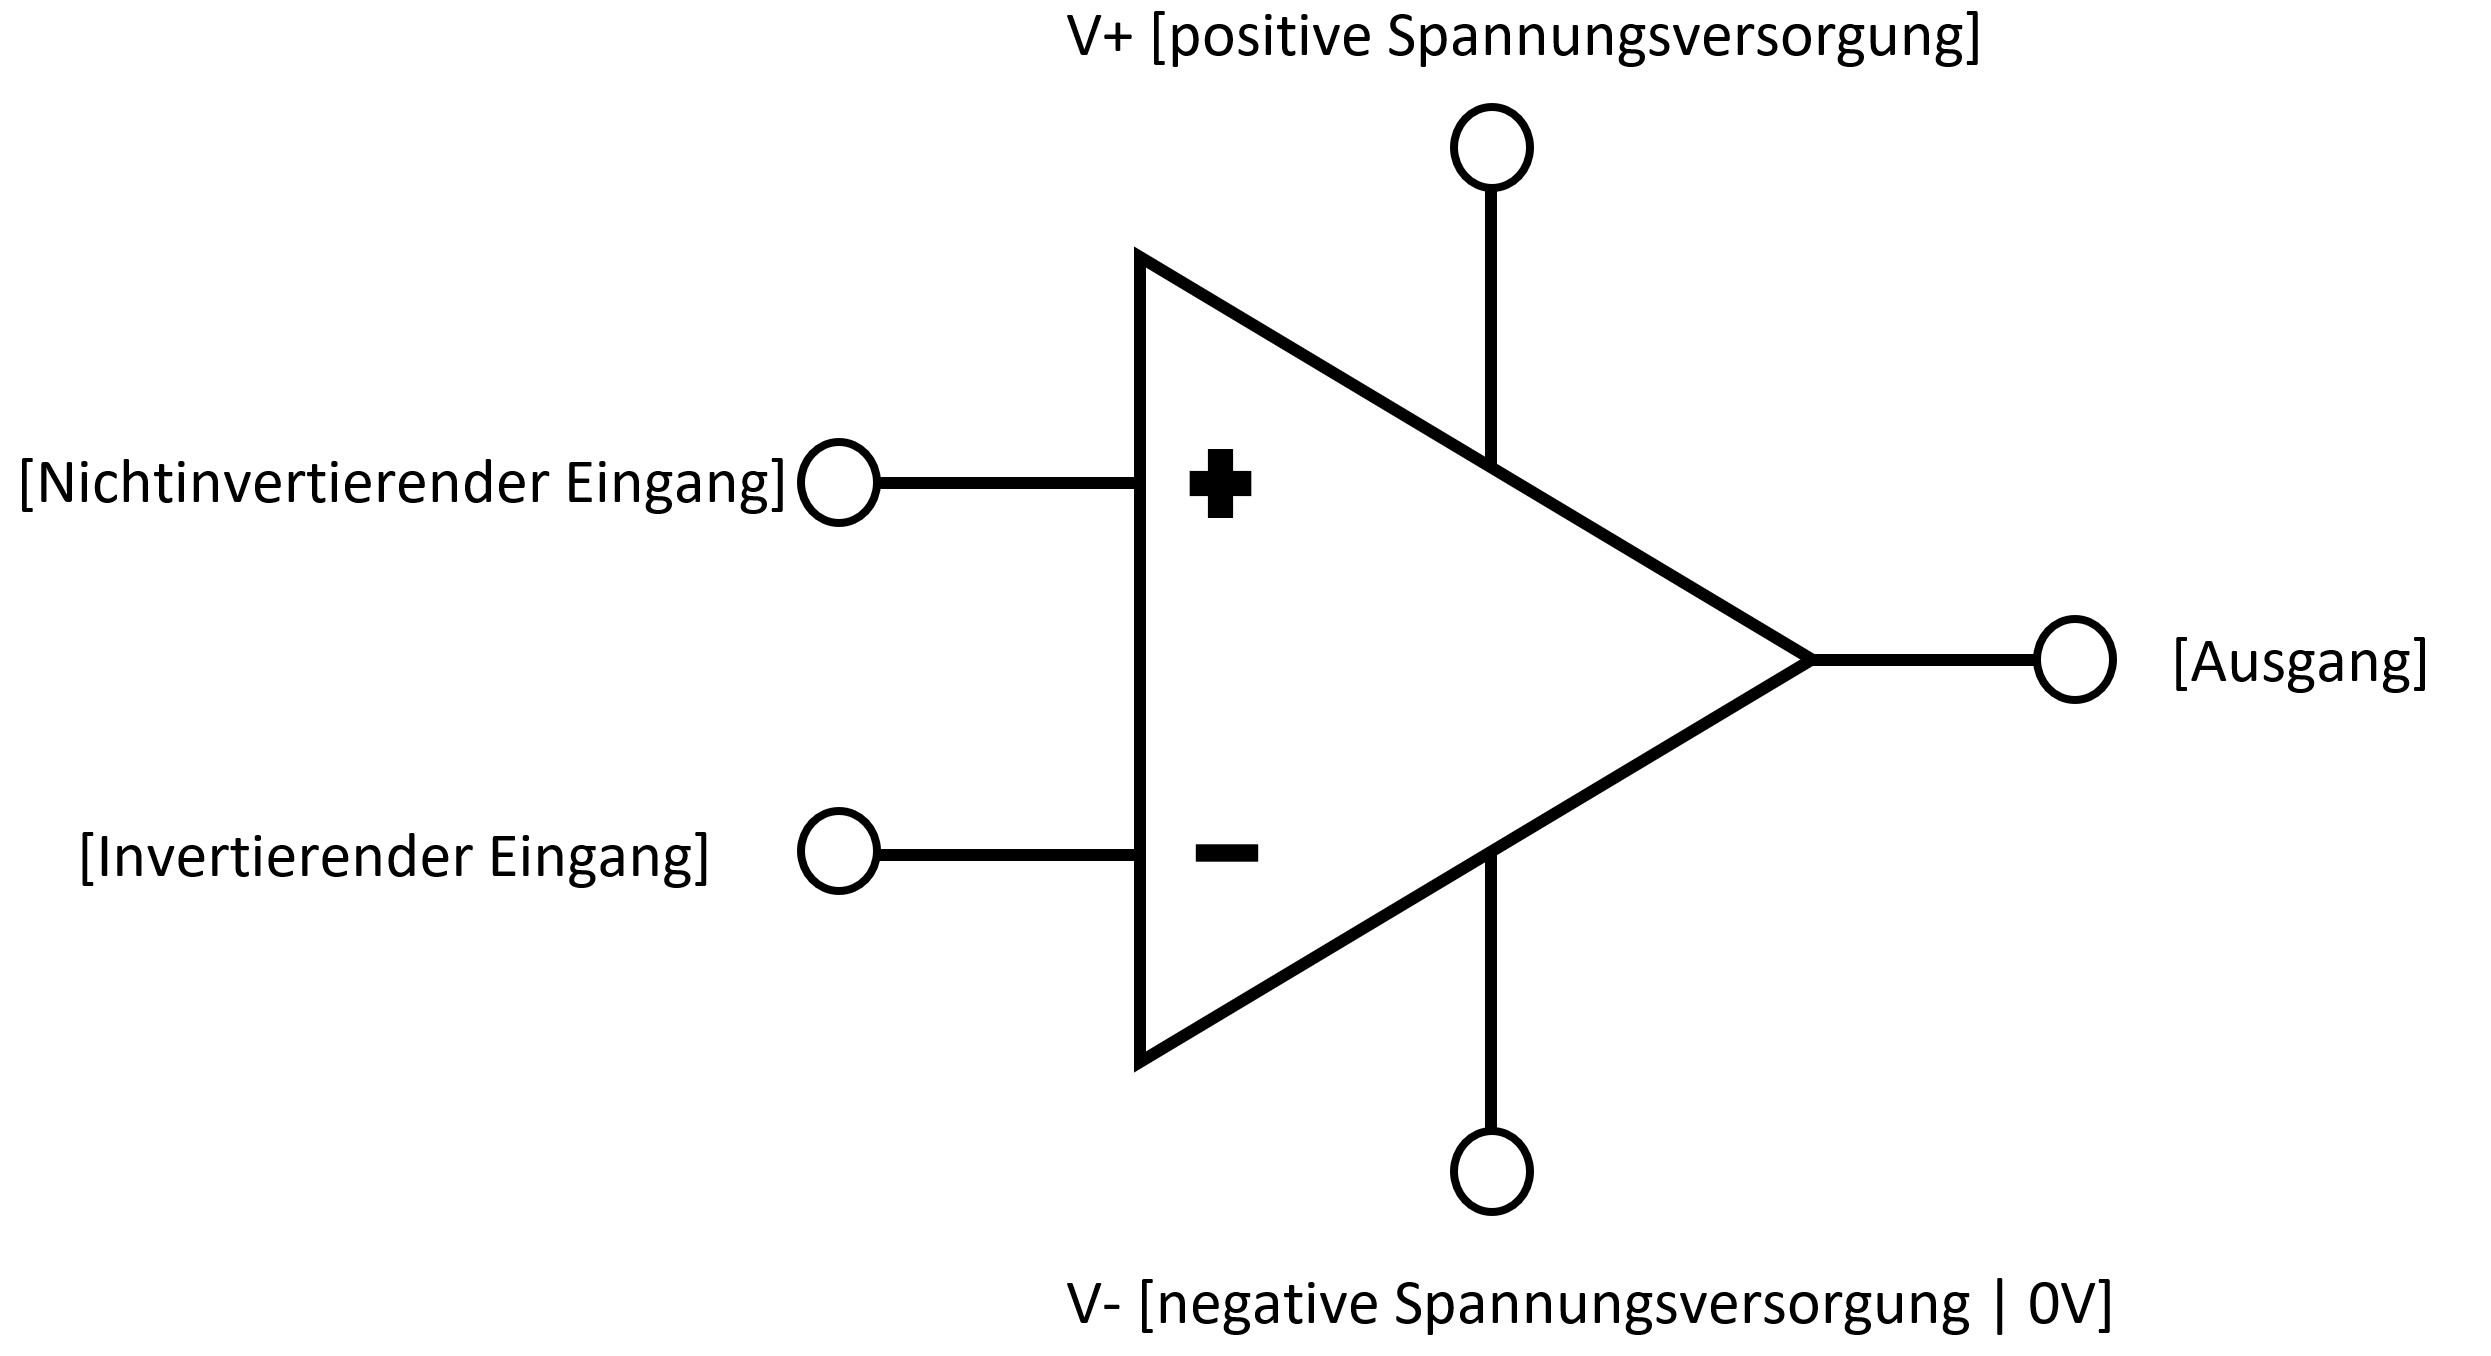
\includegraphics[width=0.7 \textwidth]{OPV.jpg}
	\caption[Operationsverstärker Anschlussschema]{Operationsverstärker Anschlussschema} 
	\gls{online:Eigen}
	\label{fig:OPV}
\end{figure}

Sie werden im Allgemeinen in Form einer integrierten Schaltung (\gls{acr:IC}) hergestellt. Die in dem Datenblatt eines Operationsverstärkers angegebenen Werte beschrieben seine Eigenschaften ausreichend. Zudem verfügt der \gls{acr:OP} über einen invertierenden $(-)$ und nicht-invertierenden $(+)$ Eingang.\cite{OP} Daraus können zwei der \gls{acr:OP}-Grundschaltungen extrahiert werden. Um das Verhältnis zwischen der Ausgangsspannung $U_{a}$ und der Eingangsspannung $U_{e}$ zu berechnen werden häufig die Parameter A oder G verwendet.\cite{tietzeElectronicCircuits2008}

\begin{equation}
	\label{equ:bsp1}
	A = \frac{U_{a}}{U_{e}}
\end{equation}

Außerdem haben \gls{acr:OP}s einen unendlich großen Eingangswiderstand und einen sehr geringen Ausgangswiderstand.
Das Ruhepotential zwischen dem invertierenden und nicht-invertierenden Eingang ist beinahe Null, weshalb zwischen beiden Eingängen keine Spannung abfällt.\cite{tietzeElectronicCircuits2008} Zudem fließt kein Steuerstrom, d.h. es fließt kein Strom in die Eingänge des \gls{acr:OP}, da es einen unendlichen Eingangswiderstand besitzt.\cite{OP}

\begin{figure}[H]
	\centering
	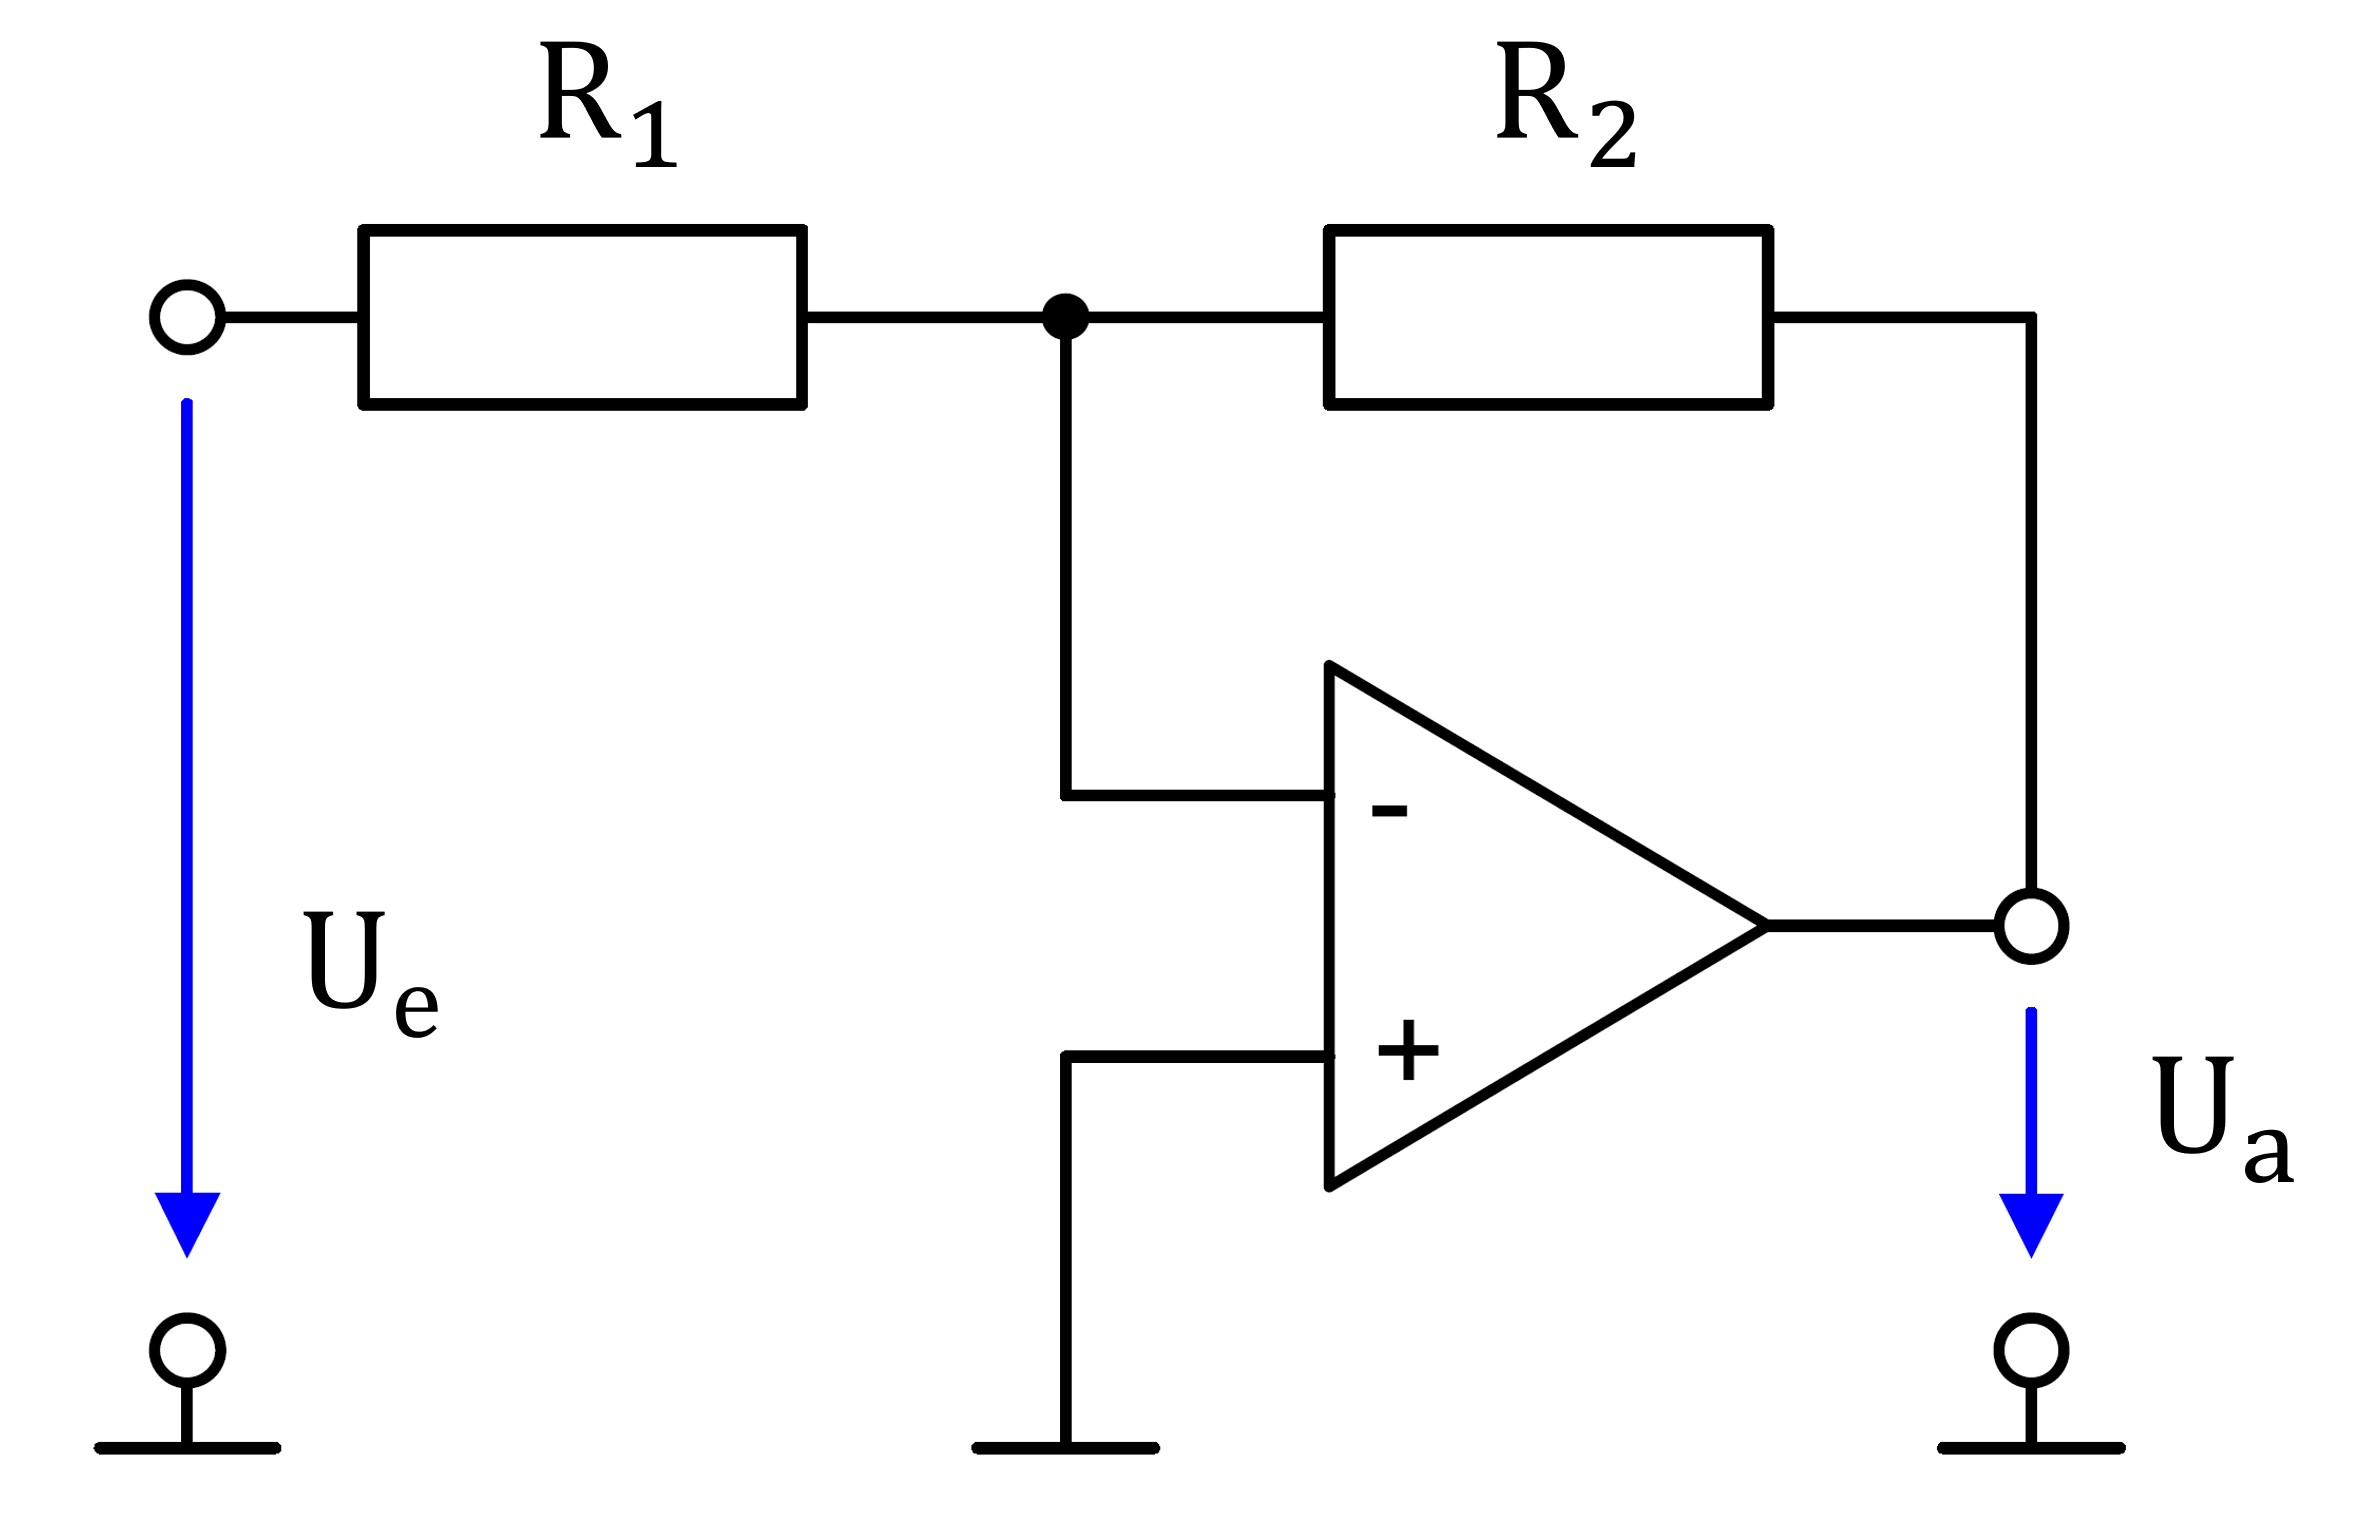
\includegraphics[width=0.7 \textwidth]{invOP.jpg}
	\caption[Invertierender Operationsverstärker]{Invertierender Operationsverstärker} 
	\gls{online:Eigen}
	\label{fig:ninvOP}
\end{figure}

Abbildung~\ref{fig:ninvOP} zeigt die klassische Schaltung eines invertierenden Operationsverstärkers mit
Rückkopplungszweig. Dieser definiert über den Widerstand $R_{2}$ die Schleifenverstärkung, indem auf den invertierten Eingang ein Teil des Ausgangssignals zurückgeführt wird.  Bei einem steigenden Ausgangssignal wird so dem steigenden Eingangssignal entgegengewirkt. Dies gewährleistet, dass das Ausgangssignal nicht unendlich verstärkt werden kann. Der invertierende Eingang wird mit Masse verbunden. Zuletzt wird hier die Spannungsverstärkung $A$ der invertierenden Grundschaltung über den Rückkopplungspfad bestimmt. Diese ergibt sich hier also zu: 

\begin{equation}
	\label{equ:bsp1}
	A = - \frac{R_{2}}{R_{1}}
\end{equation}

Das negative Vorzeichen bedeutet, dass hier eine Phasendrehung des Signals um 180$^\circ$ stattgefunden hat. Der invertierende Verstärker besitzt zudem die Fähigkeit Signale zu dämpfen. Daher wird er häufig für Filterschaltungen und messtechnische Zwecke benutzt. 

Die folgende Abbildung~\ref{fig:invOP} veranschaulicht den nicht-invertierenden Operationsverstärker in seiner Grundschaltung. Die Spannungsverstärkung berechnet sich anhand der Spannungsteiler Beziehung

\begin{equation}
	\label{equ:bsp1}
	U_{a} = U_{e} \cdot \frac{R_{1} + R_{2}}{R_{1}} = U_{e} \cdot (1+ \frac{R_{2}}{R_{1}})
\end{equation}

daraus ergibt sich dann

\begin{equation}
	\label{equ:bsp1}
	A = \frac{U_{a}}{U_{e}} = 1+ \frac{R_{2}}{R_{1}}
\end{equation}

Wegen seines kleinen Ausgangs- und großen Eingangswiderstandes eignet sich diese \gls{acr:OP}-Schaltung sehr gut als  Wechselspannungsverstärker und Impedanzwandler. Die Übertagungskennlinie ist in Abbildung~\ref{fig:aussteuer} dargestellt. 

\begin{figure}[H]
	\centering
	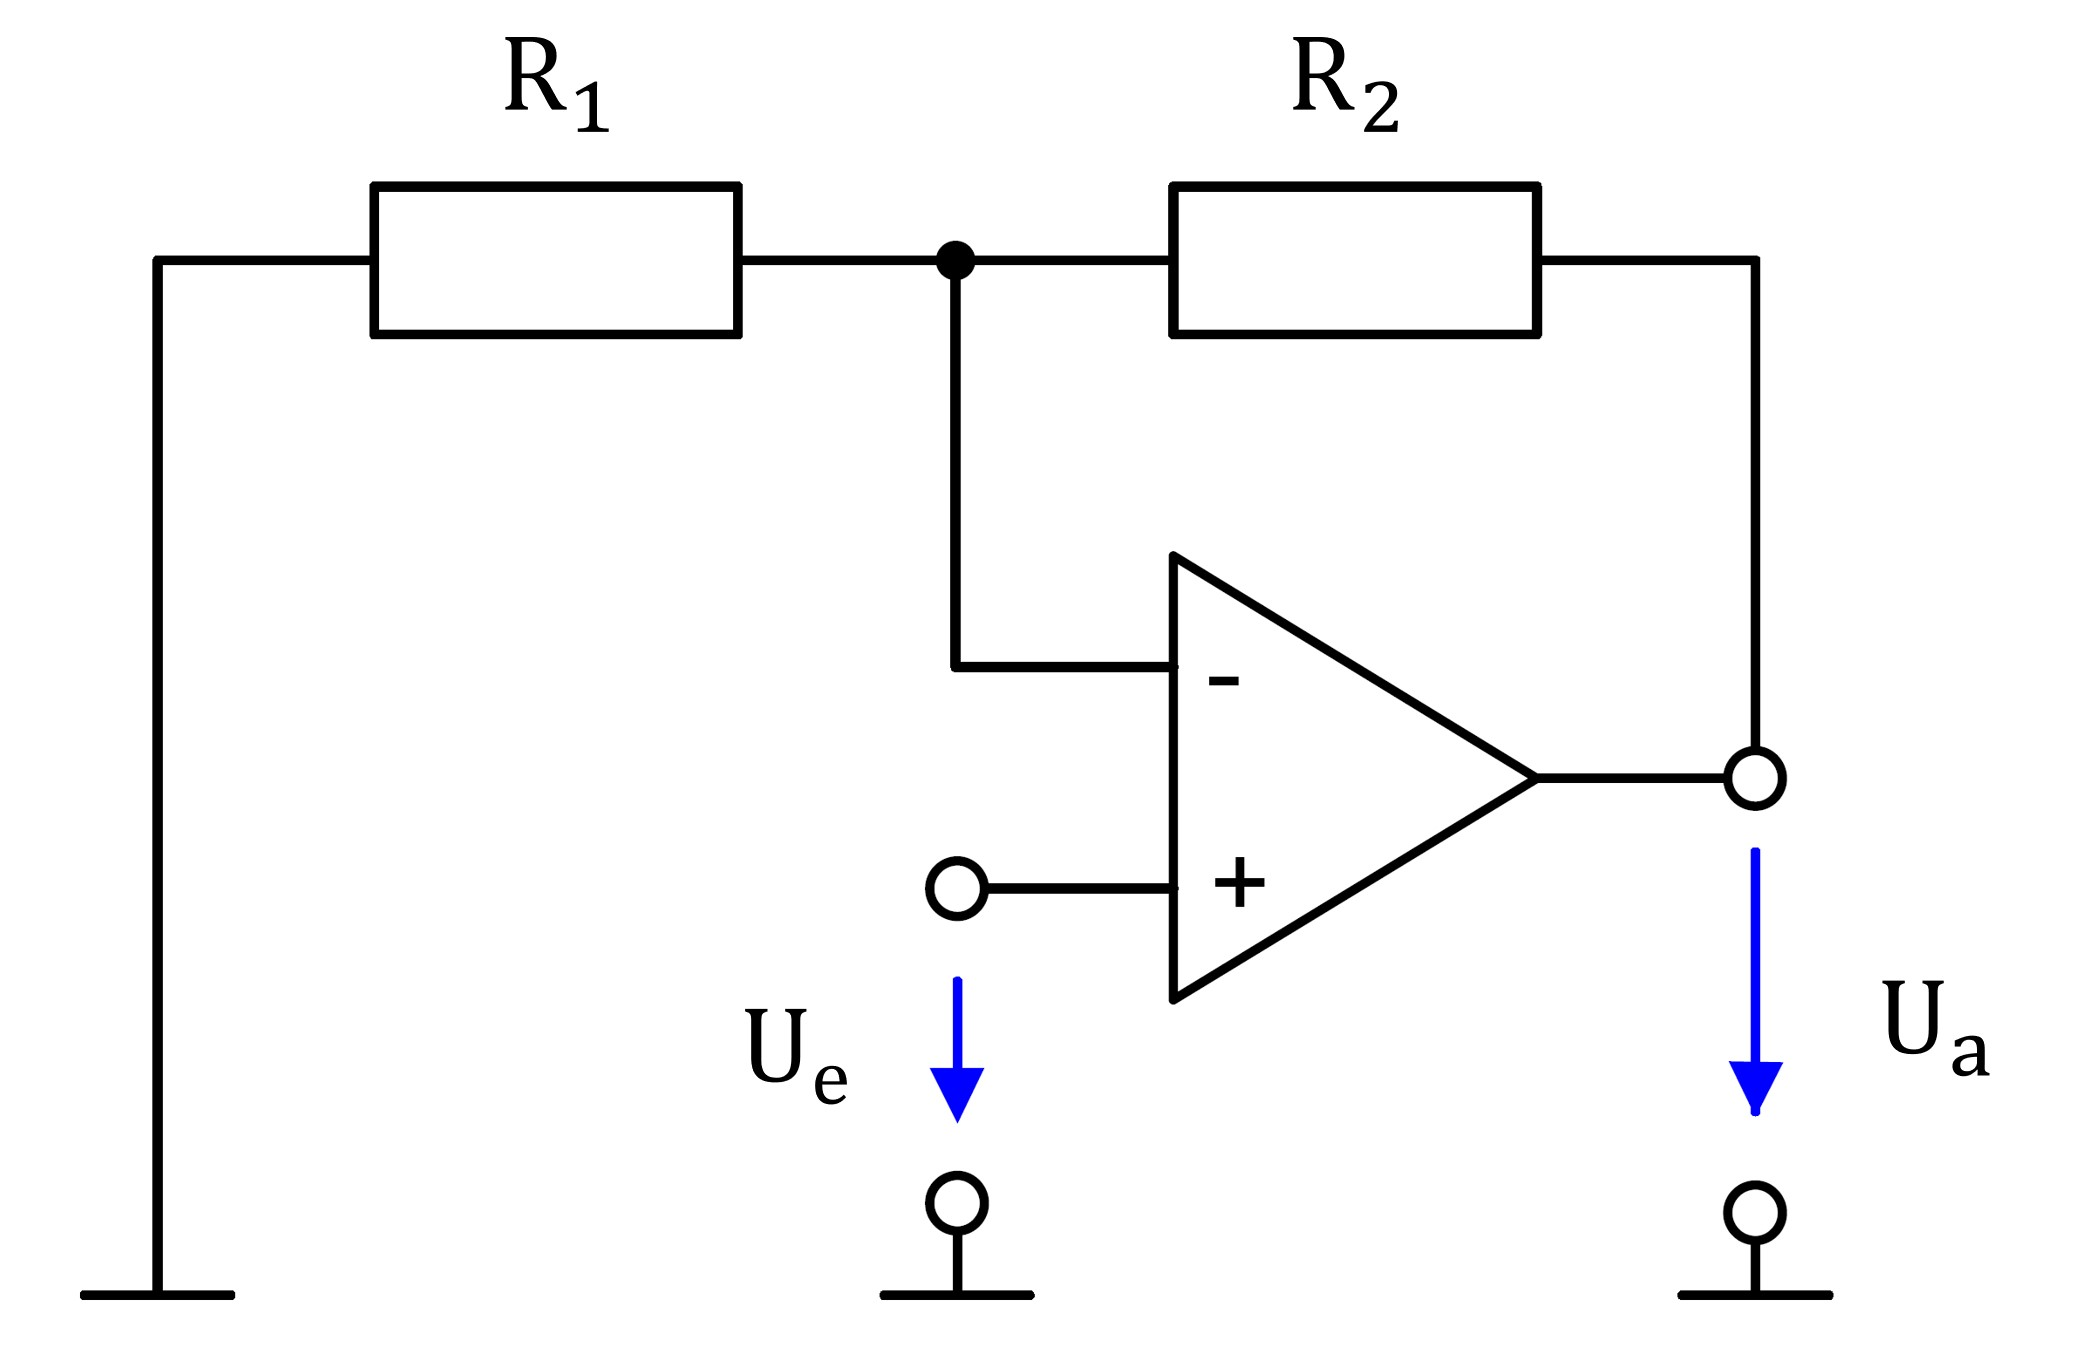
\includegraphics[width=0.7 \textwidth]{ninvOP.jpg}
	\caption[Nichtinvertierender Operationsverstärker]{Nichtinvertierender Operationsverstärker} 
	\gls{online:Eigen}
	\label{fig:invOP}
\end{figure}

Es zeigt auch die maximale Aussteuerbarkeit am Ausgang der \gls{acr:OP}s, welche innerhalb $V-$ < $U_{a}$ < $V+$ liegt. Werden entweder positive oder negative Grenzen erreicht, kann $U_{a}$ nicht weiter ansteigen. Dieser Zustand nennt sich Übersteuerung. Die klassischen Aussteuergrenzen liegen in etwa 1V unter der Versorgungsspannung (Voltage Swing).\cite{OP} Eine Ausnahme hierzu sind Rail-to-Rail Verstärker, welche sich dadurch auszeichnen, dass ihre Aussteuergrenzen der Versorgungsspannung entsprechen. 

\begin{figure}[H]
	\centering
	\includegraphics[width=0.85 \textwidth]{aussteuer.jpg}
	\caption[Theoretische Aussteuergrenze von \gls{acr:OP}s]{Theoretische Aussteuergrenze von \gls{acr:OP}s} 
	\gls{online:Eigen}
	\label{fig:aussteuer}
\end{figure} 

\newpage
\subsection{Feldeffekttransistor}
\label{subsec:mosfet}
Der am häufigsten eingesetzte Leistungsschutzschalter im Spannungsbereich bis etwa 250V ist der \gls{acr:MOSFET}.\gls{online:mosfet} Hierbei handelt es sich um eine Sonderform der Transistoren, welche auch unipolare Transistoren genannt werden. Sie besitzen einen Kanal aus Halbleitermaterial, auf dem horizontal zur Stromrichtung ein elektrisches Feld entsteht, welches den Querschnitt des Kanals verändert. Damit wird der Stromfluss durch das Bauteil geregelt. In einem \gls{acr:MOSFET} wird der Strom durch eine Spannung gesteuert. Dies ist eine Eigenschaft, welche sich im Rahmen dieser Abschlussarbeit zu Nutzen gemacht wird. Es gibt vier Grundbauformen von \gls{acr:MOSFET}. Einen \gls{acr:NMOS} und einen \gls{acr:PMOS} Typus und davon jeweils eine selbstsperrende und eine selbst leitende Variante. Im Anwendungsfall dieser Abschlussarbeit wird ein \gls{acr:NMOS} verwendet.\cite{heringElektrotechnikUndElektronik2018} 

\begin{figure}[H]
	\centering
	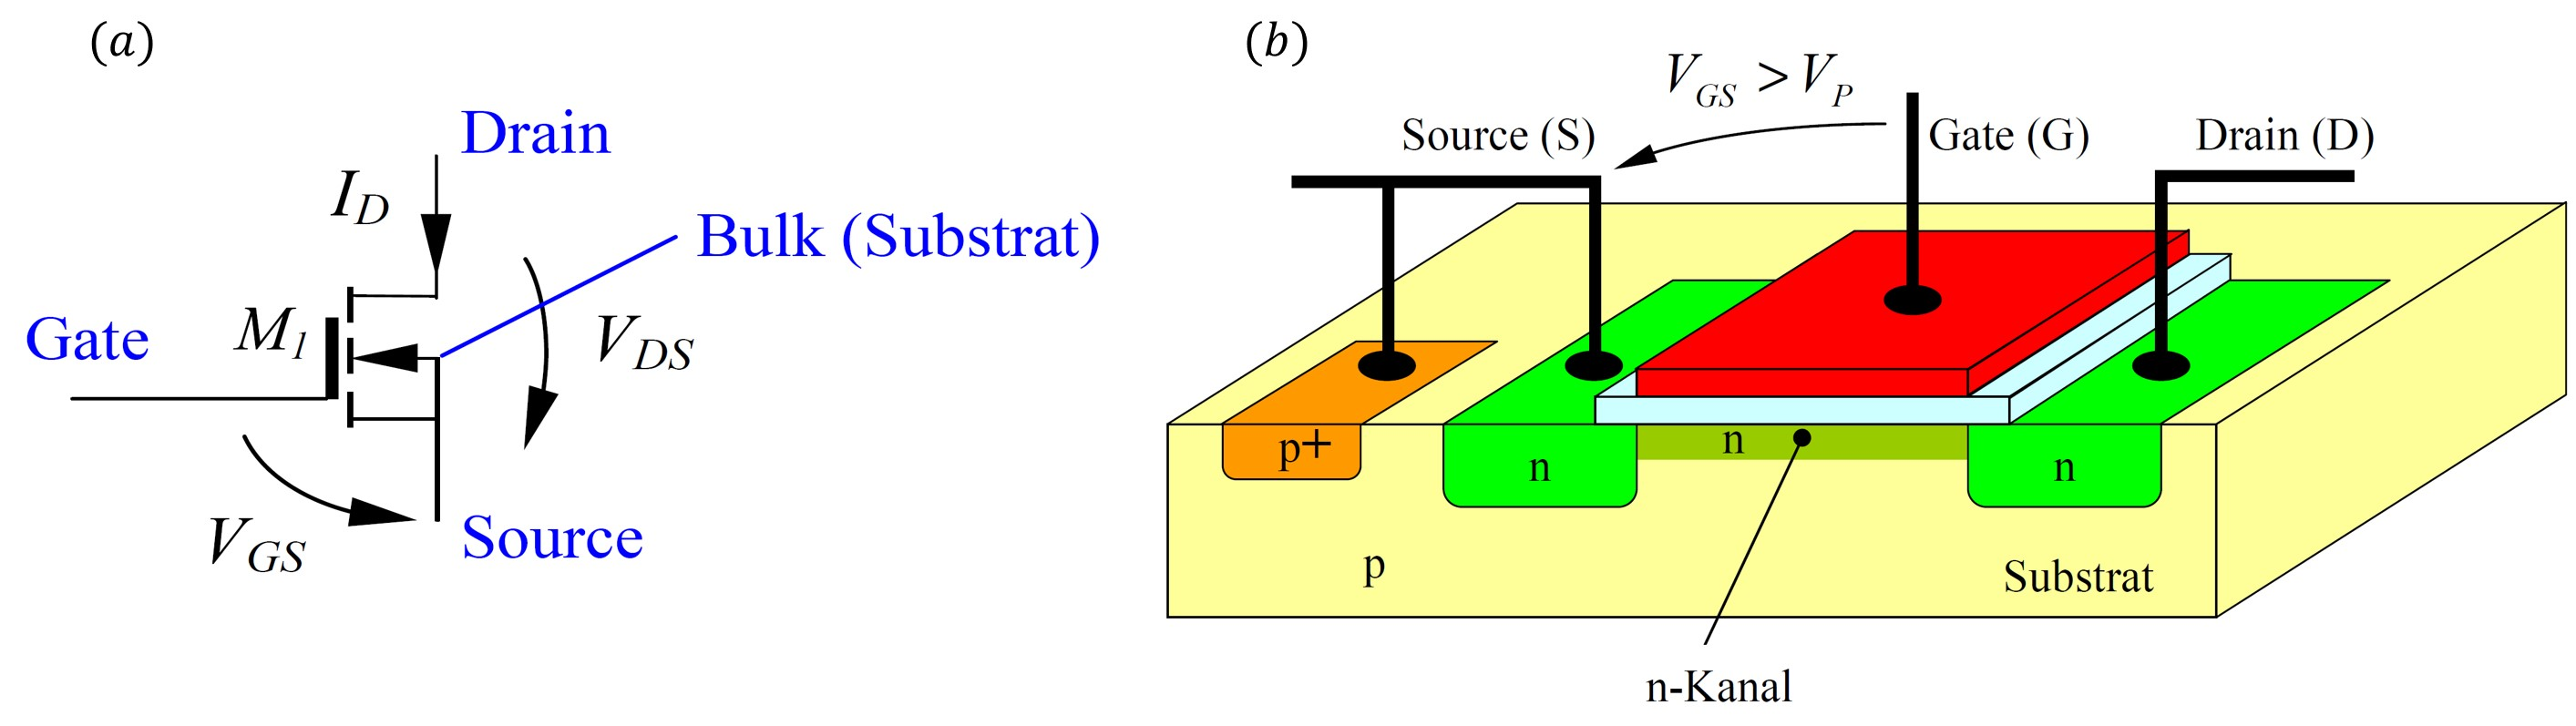
\includegraphics[width=1 \textwidth]{nmos.jpg}
	\caption[NMOS Feldeffektransistor]{NMOS Feldeffektransistor} 
	\gls{online:elektronik}
	\label{fig:nmos}
\end{figure}


In Abbildung~\ref{fig:nmos} ist unter $(a)$ das Schaltsymbol, sowie Spannungs- und Strombepfeilung eines \gls{acr:NMOS} aufgeführt. Unter $(b)$ ist der \gls{acr:NMOS} nach anlegen einer Spannung zu sehen. Dabei ist zu erkennen, dass sich unter dem Gate der n-Kanal gebildet hat. 
\subsection{Digital Potentiometer}
\label{subsec:digipot}

Um den Strom durch die \gls{acr:LED} nun digital zu regulieren und zudem die Helligkeit der \gls{acr:LED} für die Datenübertragung zu variieren, wird ein Digitalpotentiometer benötigt. Hierfür wurde der \gls{acr:IC} MCP42010 in der 10k$\ohm$–Variante mit zwei Kanälen ausgewählt. Dieses Digitalpotentiometer verfügt über eine sogenannte \gls{acr:SPI}-Schnittstelle und kann mittels eines Arduino zur Laufzeit angesteuert werden, um dessen Widerstandswert in 256 Schritten zu verändern. Dies ermöglicht eine Variation des Widerstandes in einem Bereich zwischen 52$\ohm$ (00h) und 10k$\ohm$ (FFh) in 39$\ohm$ Schritten. Bei diesem \gls{acr:SPI} handelt es sich um ein Bussystem das aus drei Leitungen besteht und für eine synchrone serielle Datenübertragung zwischen verschiedenen \gls{acr:IC}s konzipiert ist. Die vom \gls{acr:IC} vorgeschriebene Versorgungsspannung von 5V stellt der Spannungsversorgungspin des Arduino bereit. Außerdem kann dem Datenblatt des \gls{acr:IC}s entnommen werden, dass dessen Eingangsspannungsbereich an den Widerstandseingängen maximal zwischen -0,6V und +1V über der Versorgungsspannung des Bauteils liegen darf. Da der \gls{acr:IC} in dieser Schaltung mit 5V betrieben wird, dürfen die Widerstandseingänge mit einer Spannung von maximal -0,6V bis 6V belastet werden. Das ist ein äußerst wichtiges Kriterium für die Auslegung der Schaltung, da hier über die Grenzen der maximalen Amplitude entschieden werden muss, um unerwünschten Nebeneffekten oder gar einem Schaden an dem Bauteil vorzubeugen.

\begin{figure}[H]
	\centering
	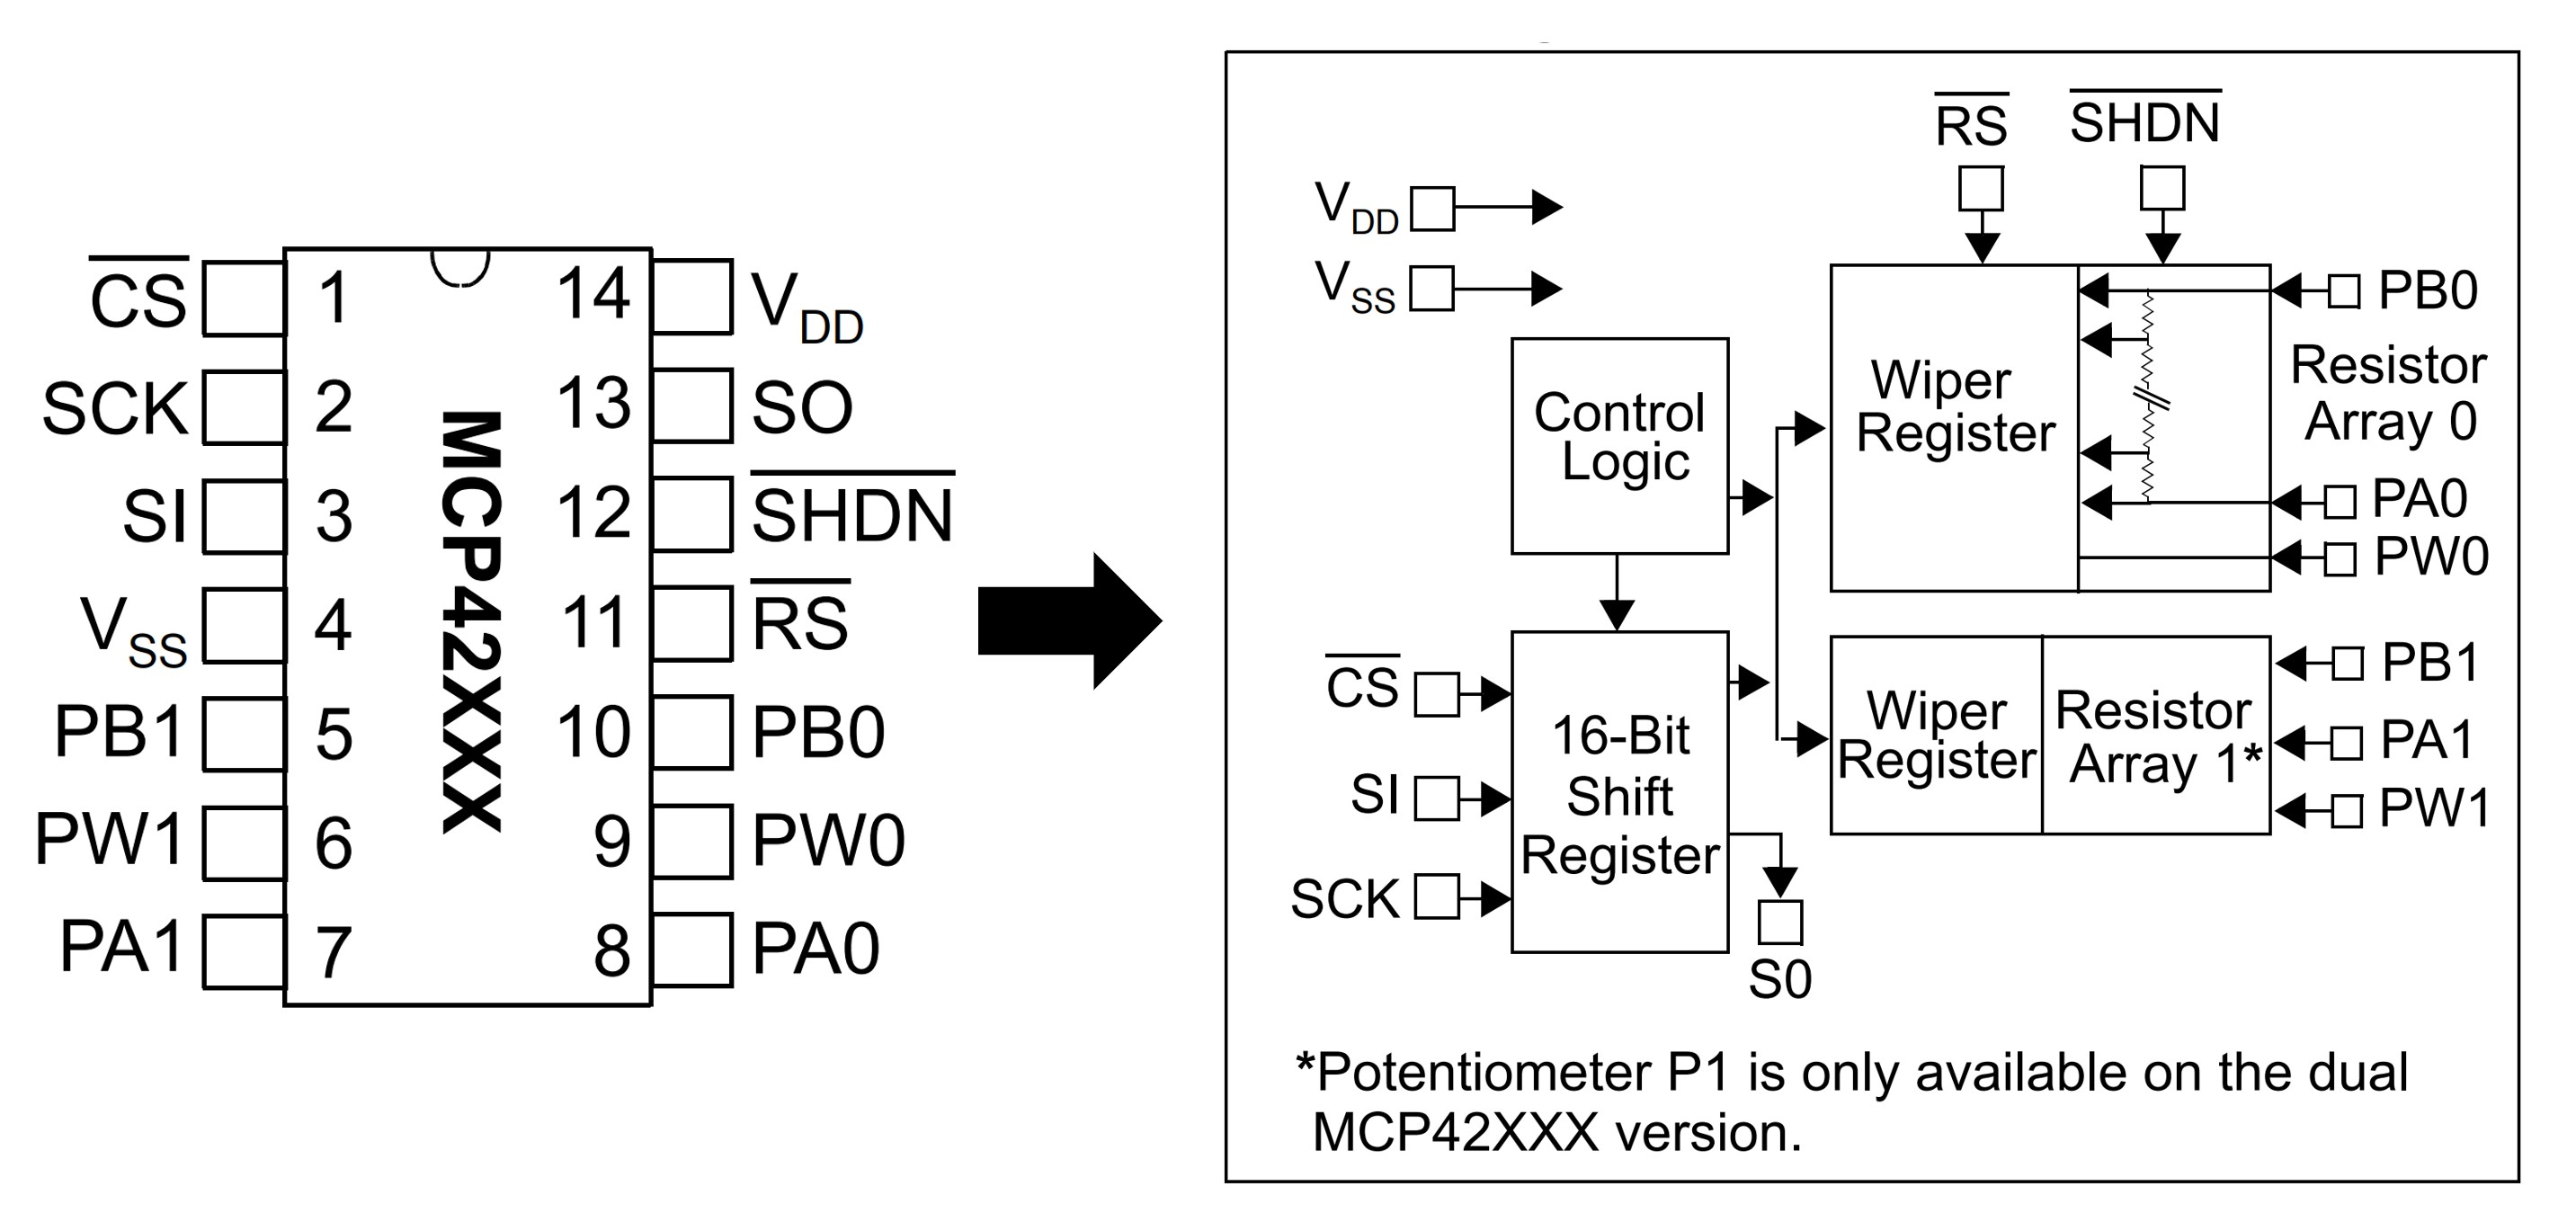
\includegraphics[width=0.7 \textwidth]{MCP.jpg}
	\caption[Aufbau des MCP42010]{Aufbau des MCP42010} 
	\gls{online:MCP42}
	\label{fig:MCP}
\end{figure}

Die Funktion der einzelnen Pins die in Abbildung~\ref{fig:MCP} sowie die Ansteuerung des \gls{acr:IC}s durch den Arduino, wird in nachfolgender Tabelle~\ref{tab:pinmcp} dargestellt. 

\begin{table}[htb]
	\begin{center}
		\begin{tabular}[H]{cccc}	
			\toprule
			\textbf{Pin Nr.} & \textbf{Name}  &\textbf{Funktion} & \textbf{Arduino Pin Nr.} \\
			\midrule
			1 & $\overline{CS}$ & Chip Select &  10 \\
			2 & SCK & Serial Clock &  13 \\
			3 & SI & Serial Data Input&  11 \\
			4 & $V_{SS}$ & Ground &  Ground \\
			5 & PB1 & Terminal B Connection For Pot 1 & X \\
			6 & PW1 & Wiper Connection For Pot 1 &  OP-1 Minus \\
			7 & PA1& Terminal A Connection For Pot 1 &  OP-1 Out  \\
			8 & PA0& Terminal A Connection For Pot 0 &  5V \\
			9 & PW0& Wiper Connection For Pot 0 & OP-2 Offset \\
			10 & PB0 & Terminal B Connection For Pot 0 &  Ground \\
			11 & $\overline{RS}$ & Reset Input & X  \\
			12 & $\overline{SHDN}$ & Shutdown Input &X\\
			13 & SO & Data Out for Daisy-Chaining & X \\
			14 & $V_{DD}$ & Power & 5V \\
			\bottomrule
		\end{tabular}
		\caption{Anschlussinformation und Pinbelegung des MCP42010 \gls{online:MCP42}}
		\label{tab:pinmcp}
	\end{center}
\end{table}

Aufgrund des Anwendungsfalls in dieser Abschlussarbeit, werden einige Pins des MCP42010 nicht benötigt und aus diesem Grund in Tabelle~\ref{tab:pinmcp} mit einem $"X"$ markiert nicht am Arduino angeschlossen.

\subsection{DC/DC Spannungswandler}
\label{subsec:dcdc}

Ein Gleichspannungswandler, oder auch \gls{acr:DC}/\gls{acr:DC}-Spannungswandler, wandelt eine der Schaltung zugeführte Eingangsgleichspannung in eine geregelte Ausgangsgleichspannung, welche ein anderes Spannungsniveau als die Eingangsspannung aufweist. Diese kann beispielsweise niedriger, höher oder auch invertiert sein.
Da die zu übertragenden Daten am Ausgang der Soundkarte als reine Wechselspannung anliegen, wird eine negative Spannungsquelle für die vorhandenen Operationsverstärker benötigt, um kein Risiko auf Datenverluste einzugehen. Hierdurch wird gewährleistet, dass die \gls{acr:OP}s auch die negativen Halbwellen des Wechselstromsignals verarbeiten können.
Gleichspannungswandler werden grundsätzlich immer dort eingesetzt, wo die zu Verfügung stehende Eingangsspannung nicht zur Versorgung der im Schaltkreis folgenden elektronischen Bauteile passt.\cite{abc} Aufgrund der Unkonventionalität, sowohl eine negative als auch eine positive Spannungsquelle simultan an die Platine anzuschließen, wandelt der \gls{acr:DC}/\gls{acr:DC}-Spannungswandler diese negative Spannung direkt auf der Platine um. Der LT1054 wird auch ”negative voltage generator” genannt. Das ist ein Bauteil, welches eine negative Ausgangsspannung erzeugt. Diese ist proportional zur Eingangsspannung $V_{CC}$. Laut typischer Beschaltung des Bauteils als einfacher \gls{acr:DC}/\gls{acr:DC}-Spannungswandler sind im Datenblatt an den Ausgängen zusätzliche Kondensatoren vorgesehen. Aufgrund dessen, dass der \gls{acr:DC}/\gls{acr:DC}-Spannungswandler mit negativen Spannungen arbeitet, ist es signifikant, im Falle der Nutzung von Elektrolytkondensatoren, auf die Polung der Kondensatoren zu achten. Jene sind unidirektional, was in Abbildung~\ref{fig:DCDC} illustriert ist. Zusätzlich ist zu erkennen, dass am negativen Ausgang des DC-DC-Wandlers nicht genau -12V anliegen sondern etwa -11.35V (Sägezahnförmig im mV-Bereich). Dies ist auf den Wirkungsgrad des DC-DC-Wandlers zurückzuführen und ist unter - Voltage Loss - im Datenblatt zu finden. 

\begin{figure}[H]
	\centering
	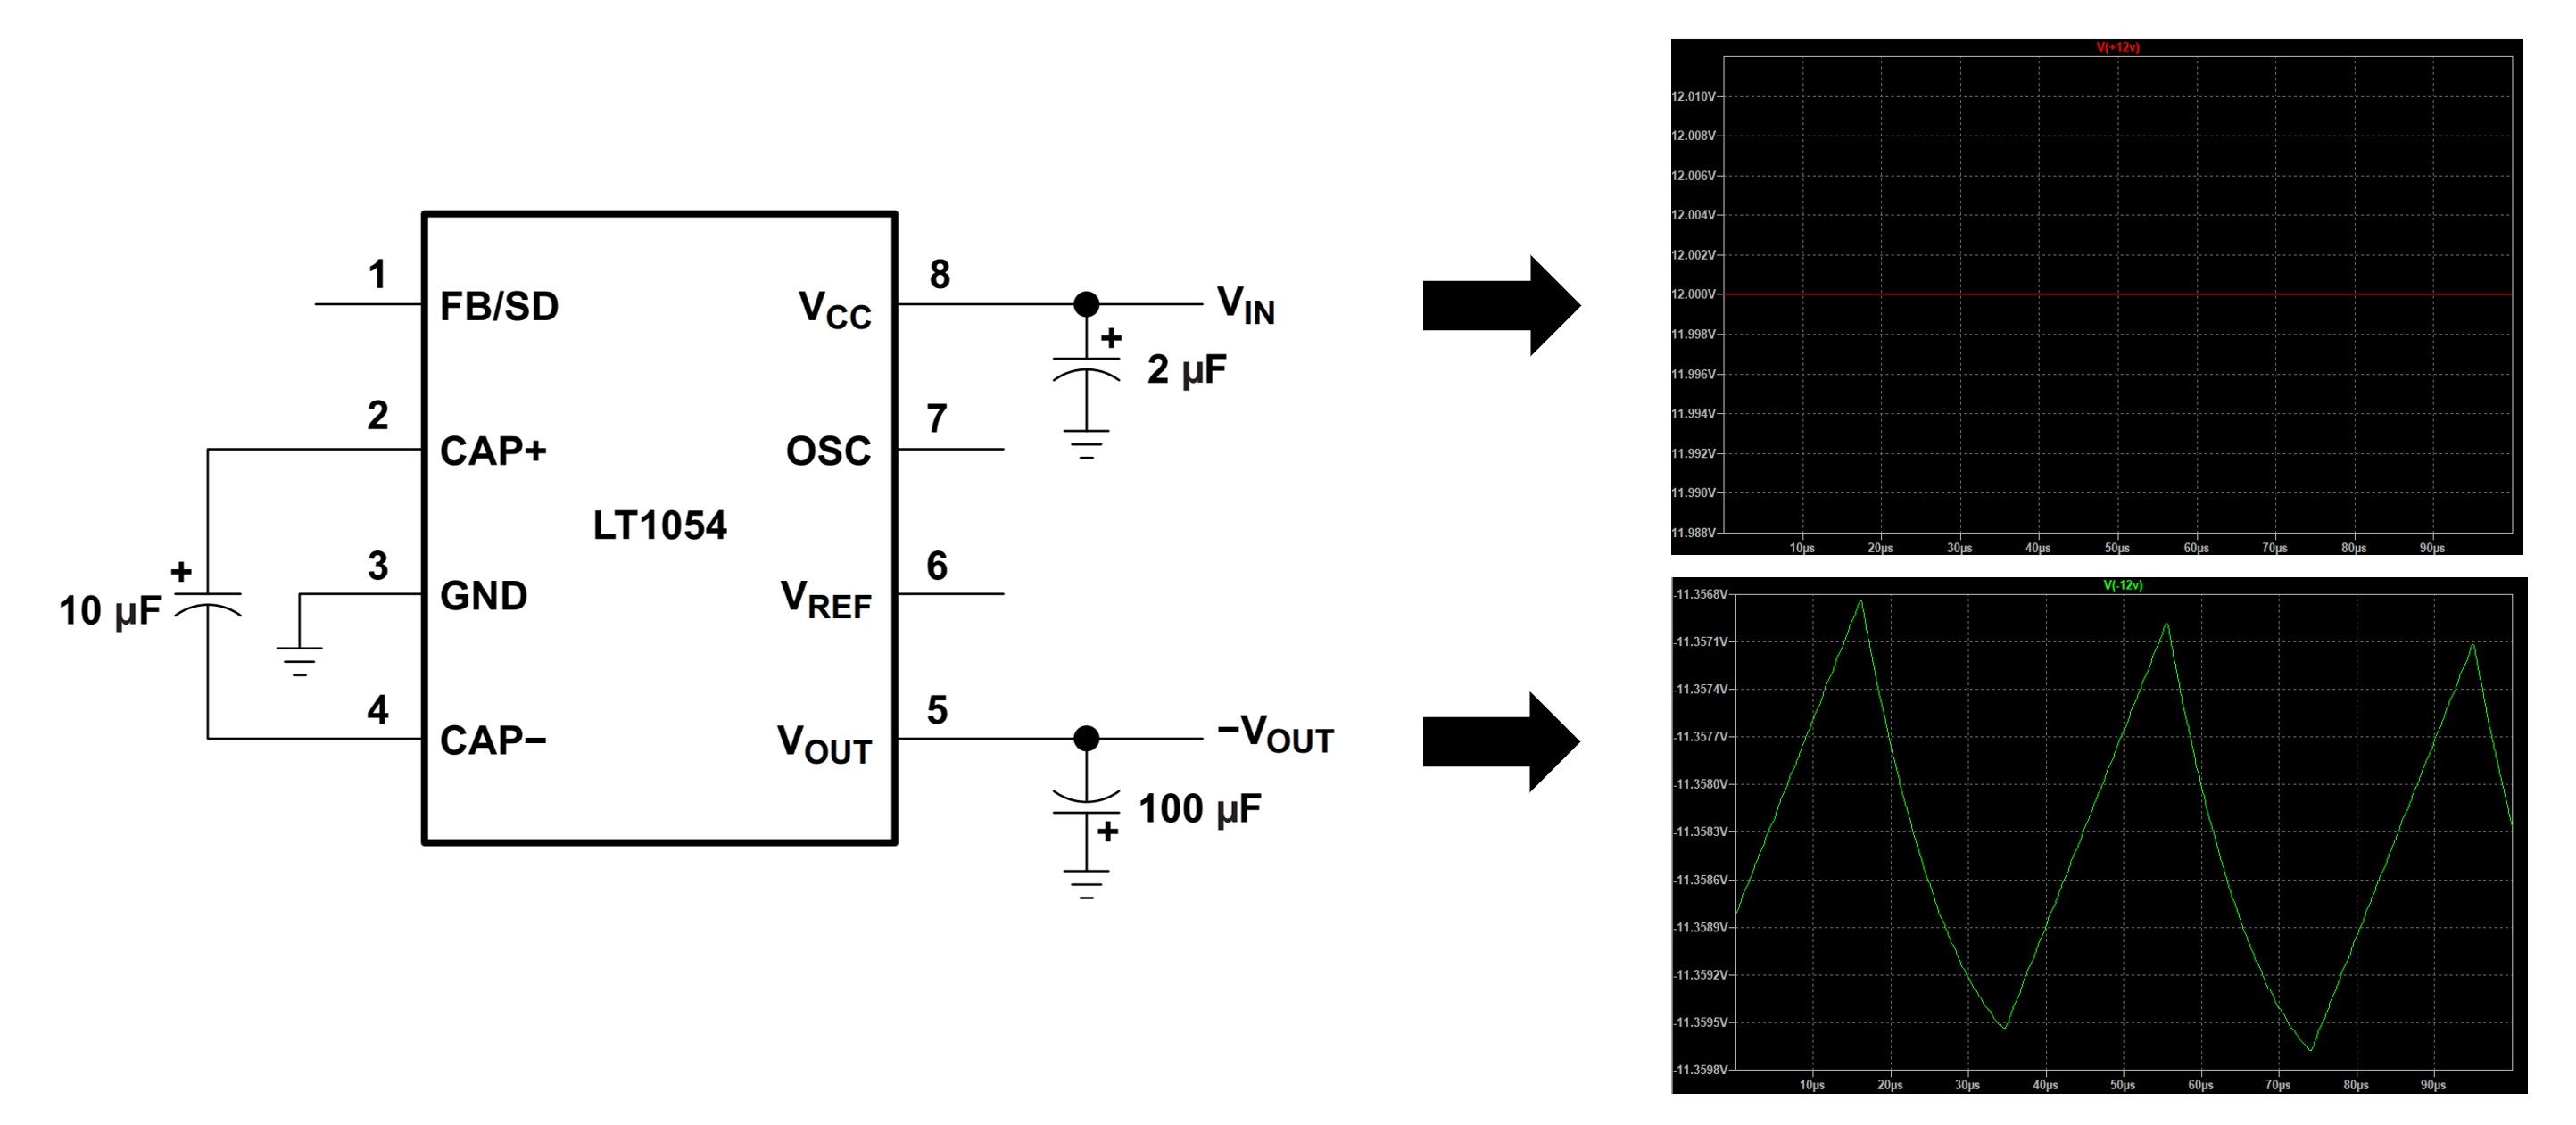
\includegraphics[width=1 \textwidth]{DCDC.jpg}
	\caption[Beschaltung und erzeugte Spannung des LT1054]{Beschaltung und erzeugte Spannung des LT1054} 
	\gls{online:Eigen}
	\label{fig:DCDC}
\end{figure}

Der Spannungswandler arbeitet außerdem intern für die Invertierung mit einer Frequenz von 25kHz. Da die zu übertragenden Daten auch nahe diesem Bereich liegen, empfiehlt es sich, den Pfad der Signalverarbeitung und den der Spannungsinvertierung auf der Platine möglichst weit auseinander zu platzieren, um möglichen parasitären Störungen vorzubeugen.


\subsection{Arduino UNO V3}
\label{subsec:unov3}

Die Arduino-Plattform besteht prinzipiell aus der auf C und C++ basierenden Entwicklungsumgebung und der zu programmierenden Hardware\gls{online:arduino}. Vorteilhaft ist hier die gute Dokumentation und eine große Menge an Bibliotheken zum Einbinden externer Hardwarekomponenten. Ein zusätzlicher Vorteil der Plattform liegt in ihrer Quelloffenheit. Alle zugehörigen Komponenten sind demnach 'Open Source'. Das hat zur Folge, dass Codes der Bibliotheken und des Bootloaders frei zur Verfügung stehen und nach Belieben verändert werden können. Auch die Architektur der Hardware ist offengelegt, weshalb Hersteller eigene kompatible Boards konstruieren und verkaufen können. Durch die Unabhängigkeit von Programmierer und Hersteller entsteht eine erschwingliche Hardware, welche bezüglich der Quelloffenheit ohne Einschränkungen programmiert werden kann.\cite{arduino}\gls{online:aufbauarduino} Diese eignet sich hervorragend zur Funktionsprogrammierung von ansteuerbaren Komponenten im analogen Signalverarbeitungspfad.

\begin{figure}[H]
	\centering
	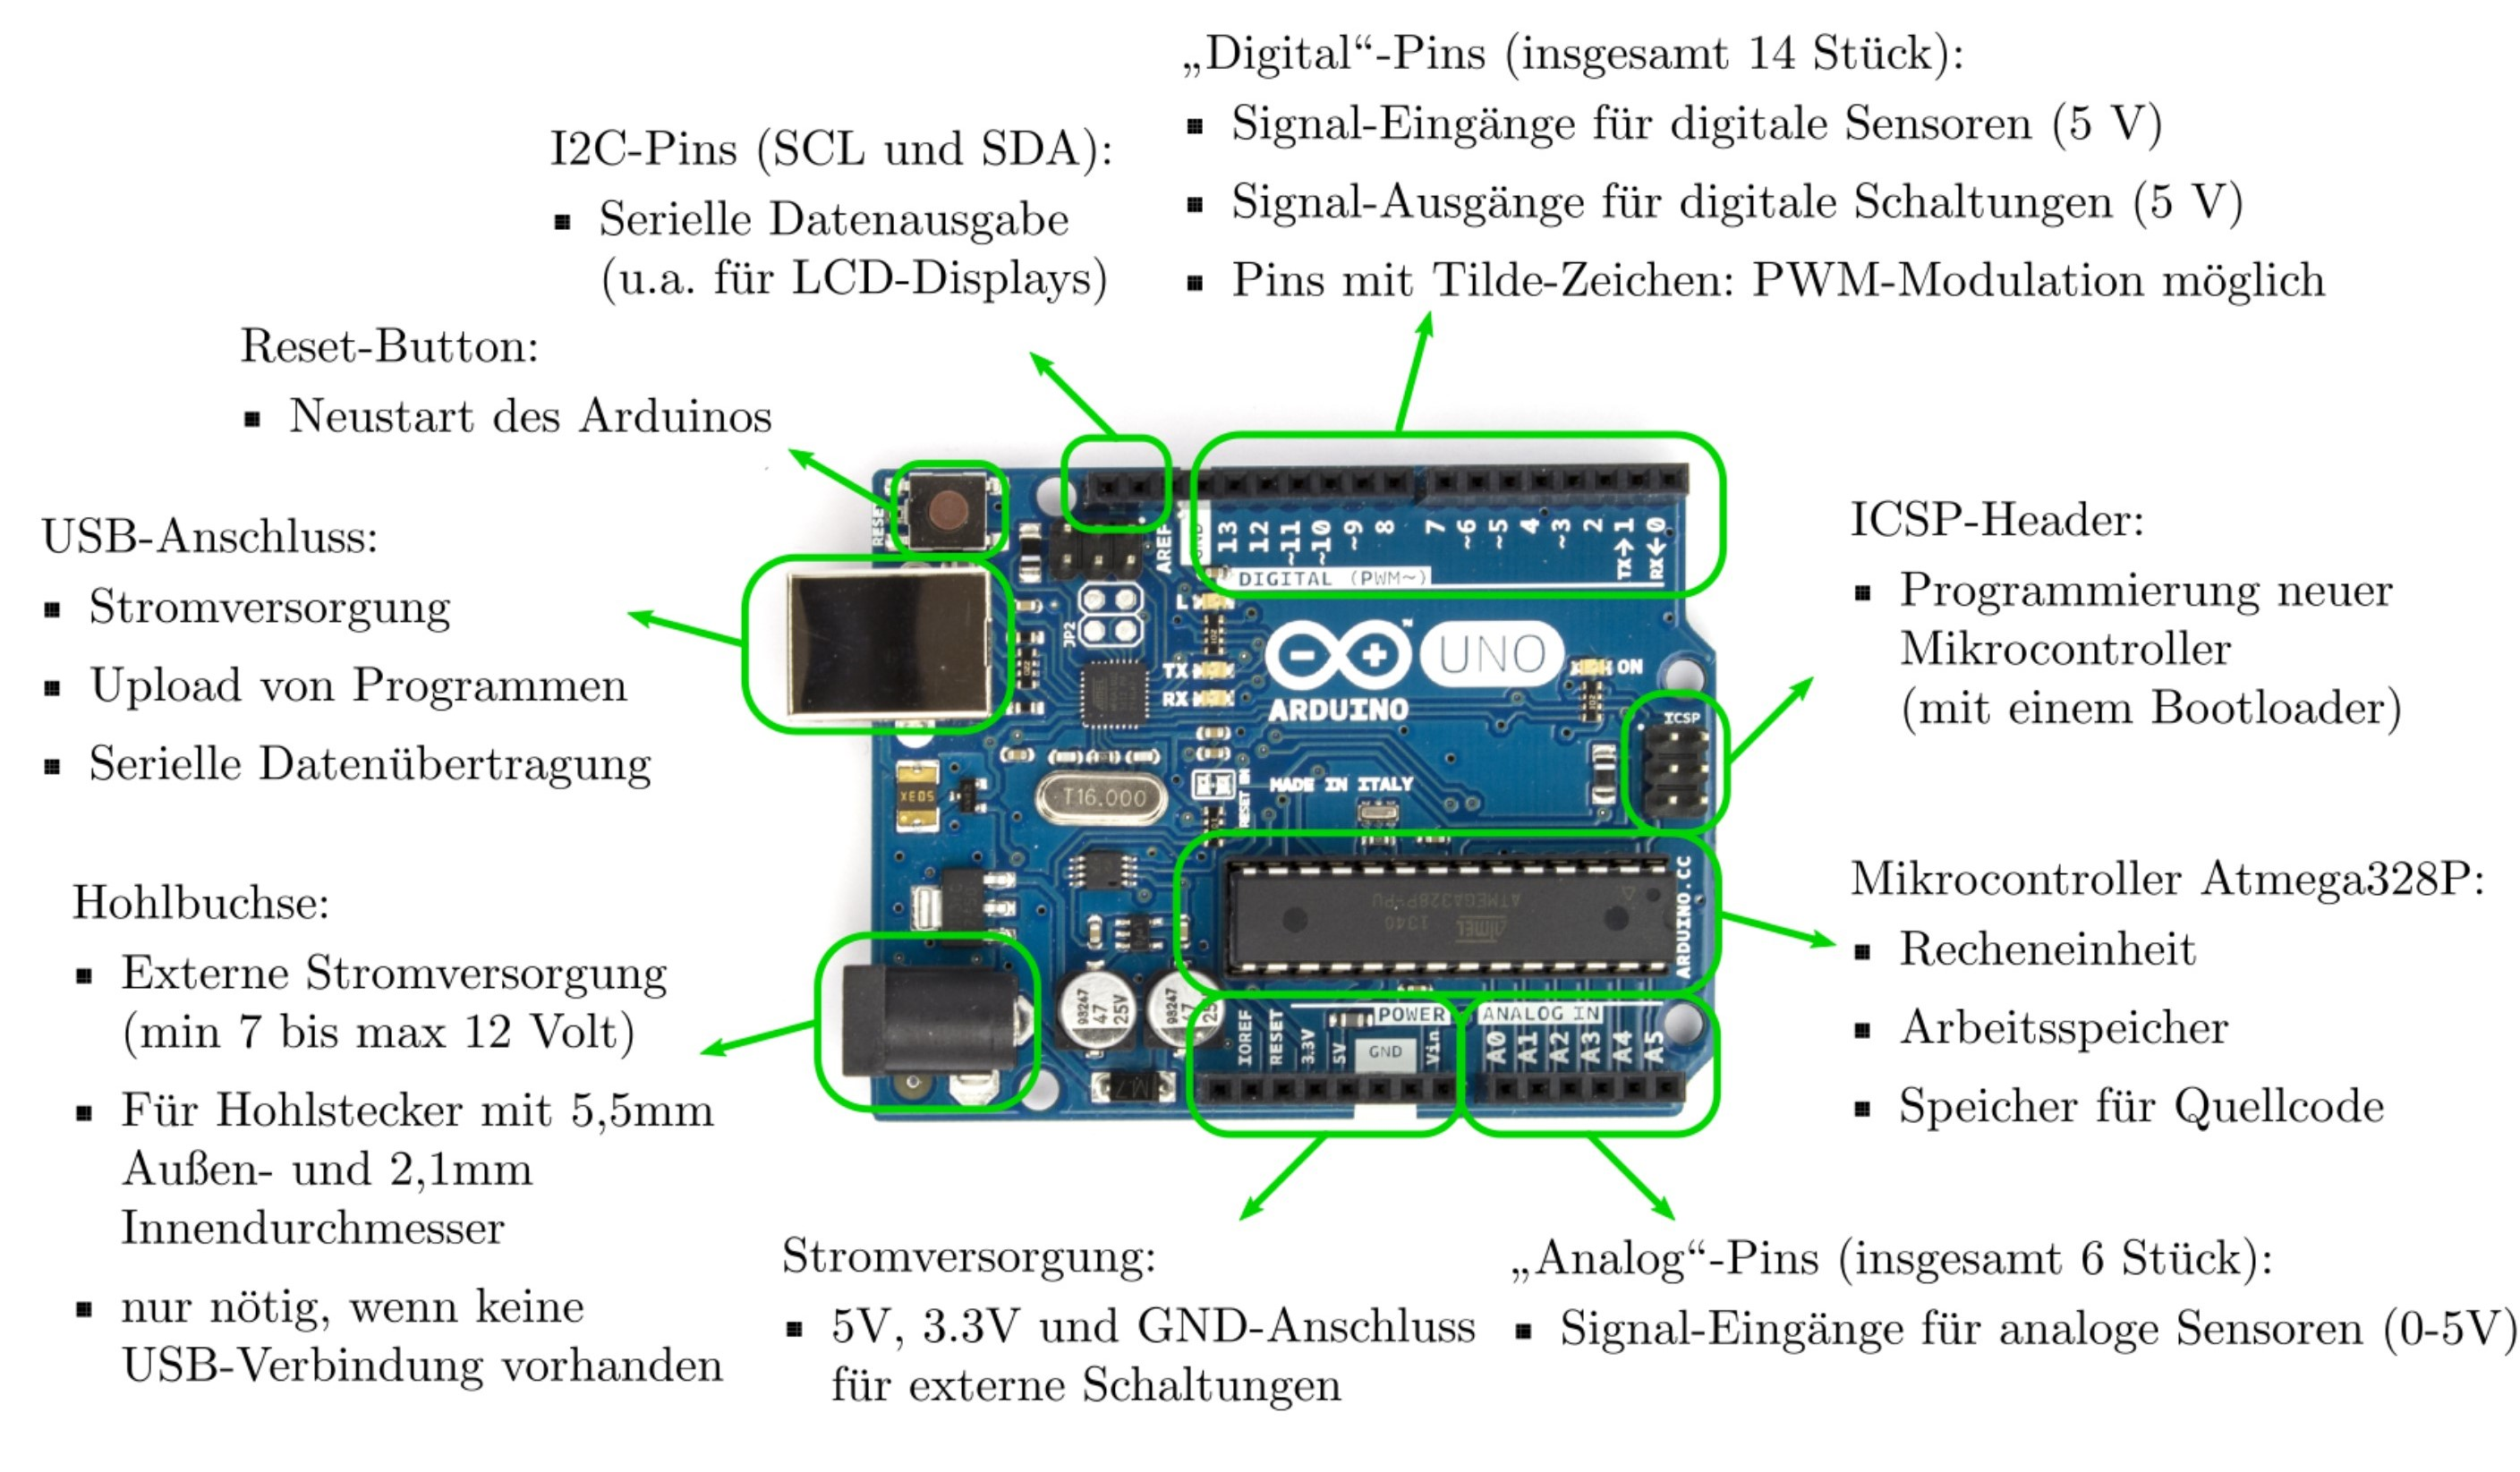
\includegraphics[width=1 \textwidth]{aufbauarduino.jpg}
	\caption[Aufbau eines Arduino UNO]{Aufbau eines Arduino UNO} 
	\gls{online:aufbauarduino}
	\label{fig:aufbauarduino}
	\end{figure}
\newpage
\section{Softwaretools}       
Nach dem die Hardwarekomponenten näher erläutert wurden, setzt sich dieses Kapitel mit den für die Umsetzung des Projektes relevanten Programmen auseinander. Diese Programme werden für die Simulation, das Design des Platinenlayouts und die Programmierung verwendet. 
 
\subsection{LT-Spice}
\label{subsec:lts}
LT-Spice ist eine \gls{acr:SPICE}-basierte Computersoftware zur Simulation analoger, elektronischer Schaltungen. Diese wurde vom Halbleiterhersteller Analog Devices (ursprünglich von \gls{acr:LT}) entwickelt. Es ist die am weitesten verbreitete und verwendete \gls{acr:SPICE}-Software in der Elektro-Simulationsbranche. Obwohl es sich um freie Software handelt, ist der LT-Spice Funktionsumfang nicht künstlich eingeschränkt.\gls{online:spice} Diese Simulationssoftware wurde im Rahmen dieser Arbeit zur Erprobung und Simulation des analogen Signalverarbeitungsschaltkreises verwendet.

\subsection{EAGLE}
\label{subsec:eagle}

\gls{acr:EAGLE} ist eine Software zum Designen und Erstellen von Leiterplattenlayouts und Schaltplänen. Die Software verfügt über einen Schaltplan- und einen Layouteditor, sowie über eine sehr umfassende Bibliothek an Bauteilen, welche sehr unkompliziert und individuell erweiterbar ist.\gls{online:eagle1}\gls{online:eagle2}

\subsection{Arduino IDE (Version 1.8.42.0)}
\label{subsec:ide}

Die Programmiersprachen, welche in der Entwicklungsumgebung zur Verfügung stehen werden sind C und in kleineren Umfängen auch C++. In den Standardbibliotheken der Entwicklungsumgebung sind die für die Programmierung erheblichsten Funktionen zusammengefasst. Um weitere Funktionen zu nutzen, können dementsprechend zusätzliche Bibliotheken eingebunden werden. 
Der Editor mit integriertem Compiler ist ein weiterer Bestandteil des \gls{acr:IDE}. In diesem wird der Code geschrieben, kompiliert und auf das Board überspielt. User benötigen also nur eine Software, um ihre Mikrocontroller in vollen Umfängen nutzen zu können. Dieses \gls{acr:IDE} bietet außerdem die Möglichkeit, Bibliotheken oder gar Programmbeispiele herunterzuladen.\cite{arduino}

\begin{figure}[H]
	\centering
	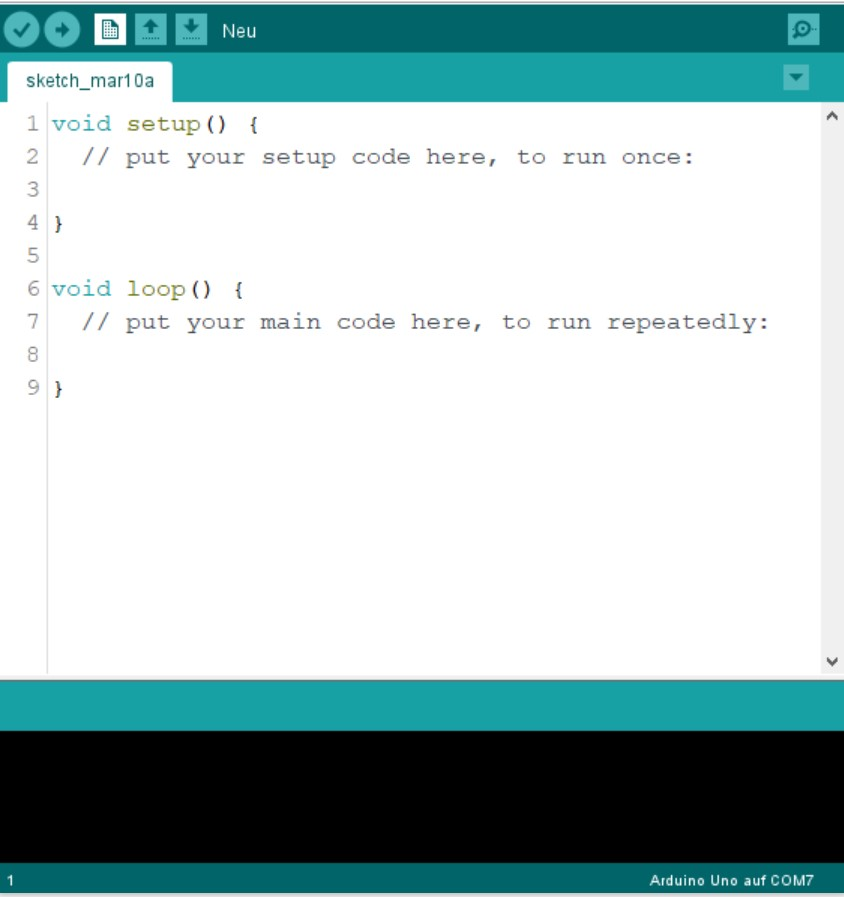
\includegraphics[width = 0.6 \textwidth ]{ide.jpg}
	\caption[Arduino \gls{acr:IDE}]{Arduino \gls{acr:IDE}}\gls{online:Eigen}
	\label{fig:ide}
\end{figure}

Arduino-Programme basieren immer auf einem einheitlichen Grundaufbau. In Abbildung ~\ref{fig:ide} ist dieser zu erkennen. Es sind zwei Funktionen namens setup() und loop() deklariert. Die Funktion setup() wird einmalig zu beginn des Programms aufgerufen, während loop() direkt im Anschluss aufgerufen wird und in einer Endlosschleife ausgeführt wird bis der Mikrocontroller stromlos geschaltet wird. Oberhalb der Funktion setup() können außerdem noch Präprozessorbefehle implementiert werden.

\subsection{Dream (Version 2.2.1)}
\label{subsec:dreamsoft}
Die Software Dream bietet eine Möglichkeit um Radiosignale auf dem Computer zu empfangen und auch zu senden. Sie war ursprünglich als Forschungsprojekt des Fraunhofer Instituts angesetzt. Signale, welche nicht über den \gls{acr:PC} empfangen werden können, werden über den Mikrofon-Eingang der Soundkarte empfangen.
Bei alldem benutzt das Konzept internationale Direktiven für Amateurfunk, Radio und Informationsdienste. Diese Eigenschaft ermöglicht es dem Anwender, \gls{acr:FM}, \gls{acr:AM} und \gls{acr:DRM} zu senden und zu empfangen. Außerdem visualisiert die Software in Echtzeit zahlreiche Daten, Statistiken und Diagramme des empfangenen Signals. \gls{online:dream} Die Modulation und das Senden des \gls{acr:OFDM}-Signals über die konstruierte Hardware erfolgt durch diese Software und wird in den folgenden Kapiteln noch weiter intensiviert.